\documentclass{tufte-handout} % A4 paper and 11pt font size
%\usepackage[activate={true,nocompatibility},final,tracking=true,kerning=true,spacing=true,factor=1100,stretch=10,shrink=10]{microtype}
\usepackage[T1]{fontenc} % Use 8-bit encoding that has 256 glyphs
\usepackage{mathpazo} % Use the Adobe Utopia font for the document - comment this line to return to the LaTeX default
\usepackage[english]{babel} % English language/hyphenation
\usepackage{amsmath,amsfonts,amsthm, amssymb} % Math packages
\usepackage{pgf,tikz}
\usetikzlibrary{positioning,matrix,arrows}
\usepackage{float}
\usepackage{tikz-cd}
\usepackage{caption}
\usepackage{stmaryrd}
\usepackage{multicol}
\usepackage{booktabs}
\usepackage{verbatim}
\usepackage{bussproofs}
\usepackage{lipsum} % Used for inserting dummy 'Lorem ipsum' text into the template
\usepackage{sectsty} % Allows customizing section commands
\allsectionsfont{\normalfont \bfseries} % Make all sections centered, the default font and small caps
\usepackage{hyperref}
\usepackage{enumerate}
\usepackage{pythonhighlight}
\usepackage{fancyhdr} % Custom headers and footers
\pagestyle{fancyplain} % Makes all pages in the document conform to the custom headers and footers
\fancyhead{} % No page header - if you want one, create it in the same way as the footers below
\fancyfoot[L]{} % Empty left footer
\fancyfoot[C]{} % Empty center footer
\fancyfoot[R]{\thepage} % Page numbering for right footer
\renewcommand{\headrulewidth}{0pt} % Remove header underlines
\renewcommand{\footrulewidth}{0pt} % Remove footer underlines
\setlength{\headheight}{13.6pt} % Customize the height of the header
\allowdisplaybreaks
%--------Theorem Environments--------
%theoremstyle{plain} --- default
\newtheorem{thm}{Theorem}
\newtheorem{cor}[thm]{Corollary}
\newtheorem{prop}[thm]{Proposition}
\newtheorem{facts}[thm]{Facts}
\newtheorem{fact}[thm]{Fact}
\newtheorem{clm}[thm]{Claim}
\newtheorem{lem}[thm]{Lemma}
\newtheorem{conj}[thm]{Conjecture}
\newtheorem{quest}[thm]{Question}

\theoremstyle{definition}
\newtheorem{defn}[thm]{Definition}
\newtheorem{defns}[thm]{Definitions}
\newtheorem{con}[thm]{Construction}
\newtheorem{exmp}[thm]{Example}
\newtheorem{exmps}[thm]{Examples}
\newtheorem{notn}[thm]{Notation}
\newtheorem{notns}[thm]{Notations}
\newtheorem{addm}[thm]{Addendum}
\newtheorem{exer}[thm]{Exercise}

\theoremstyle{remark}
\newtheorem{rem}[thm]{Remark}
\newtheorem{rems}[thm]{Remarks}
\newtheorem{warn}[thm]{Warning}
\newtheorem{sch}[thm]{Scholium}

\newcommand{\bra}[1]{\left(#1\right)}
\newcommand{\sbra}[1]{\left[#1\right]}
\newcommand{\Mod}[1]{\ (\text{mod}\ #1)}
\newcommand{\op}[1]{#1^{\text{op}}}
\newcommand{\R}{\mathbb{R}}
\newcommand{\N}{\mathbb{N}}
\newcommand{\Z}{\mathbb{Z}}
\newcommand{\mE}{\mathcal{E}}
\newcommand{\mP}{\mathcal{P}}
\renewcommand{\C}{\mathbb{C}}
\newcommand{\Q}{\mathbb{Q}}
\newcommand{\F}{\mathbb{F}}
\newcommand{\bA}{\mathbb{A}}
\newcommand{\bH}{\mathbb{H}}
\newcommand{\one}{\mathbb{1}}
\newcommand{\mC}{\mathcal{C}}
\newcommand{\0}{\textsf{0}}
\newcommand{\1}{\textsf{1}}
\newcommand{\mO}{\mathcal{O}}
\newcommand{\mX}{\mathcal{X}}
\newcommand{\mS}{\mathcal{S}}
\newcommand{\lp}{{\mathfrak{p}}}
\renewcommand{\P}{\mathbb{P}}
\newcommand{\E}{\mathbb{E}}
\newcommand{\AP}{\text{AP}}
\newcommand{\Loc}{\text{Loc}}
\newcommand{\Eval}{\text{Eval}}
\newcommand{\Eff}{\text{Effect}}
\newcommand{\Vars}{\text{Vars}}
\newcommand{\Cond}{\text{Cond}}
\newcommand{\tmid}{\kern-0.20ex\mid\kern-0.20ex\mid\kern-0.20ex \mid}
\newcommand{\interior}[1]{
	{\kern0pt#1}^{\mathrm{o}}
}
\newcommand{\dmid}{\kern-0.20ex\mid\kern-0.20ex\mid}
\newcommand{\rest}[2]{#1 \kern-0.65ex\upharpoonright \kern-0.55ex #2}
\newcommand{\action}[1]{\stackrel{#1}{\rightarrow}}
\DeclareMathOperator{\Tr}{Tr}
\DeclareMathOperator{\Dom}{Dom}
\DeclareMathOperator{\ext}{ext}
\newcommand{\norm}[1]{\left\lVert #1 \right\rVert}
\newcommand{\inp}[2]{\left\langle #1, #2 \right\rangle}
\newcommand{\sem}[2]{\llbracket #1 \rrbracket_{#2}}
\newcommand{\vSim}{\mathrel{\scalebox{1}[1.5]{$\shortmid$}\mkern-3.5mu\raisebox{0.1ex}{$\approx$}}}
\newcommand{\Pos}{\mathrel{\text{Pos}}}
\newcommand{\Neg}{\mathrel{\text{Neg}}}
\newcommand{\pref}{\text{pref}}
\newcommand{\cl}{\text{cl}}
\newcommand{\lang}{\mathcal{L}_{\omega}}


\newenvironment{bprooftree}
{\leavevmode\hbox\bgroup}
{\DisplayProof\egroup}

\geometry{
	left=13mm, % left margin
	textwidth=130mm, % main text block
	marginparsep=8mm, % gutter between main text block and margin notes
	marginparwidth=55mm % width of margin notes
}
\fontsize{10}{20}\selectfont
%----------------------------------------------------------------------------------------
%	TITLE SECTION
%----------------------------------------------------------------------------------------

\title{	
	\normalfont\normalsize 
	{ENS Lyon - Winter 2020} \\ [0pt] % Your university, school and/or department name(s)
	\huge Lecture Notes - SV% The assignment title
}\author{Ralph Sarkis} % Your name
\date{\vspace{-5pt}\normalsize March 31, 2020} % Today's date or a custom date

\begin{document}
\justifying 
\maketitle
\begin{abstract}
	These are lecture notes taken during the \textit{Semantics and Verification} classes taught by Colin Riba in winter 2020.
\end{abstract}
\tableofcontents
\begin{quest}
	What is \textbf{Semantics and Verification}?
\end{quest}
While it is easy enough to describe how a simple program is executed, it is virtually impossible to infer the precise behavior of a machine running a large piece of code. Even more so if the latter contains randomness, parallelism or other complex features now available in most devices. The field of semantics is concerned with circumventing the useless details of the machine implementation by giving formal mathematical meaning to programs. This lets us reason rigorously about their execution or any interesting properties that they have.

Verification is a terminology for methods that, given a program in an abstract language and a property usually in another language, automatically verify whether the program satisfies the property. A common object that is used to describe programs is a \textbf{transition system}\footnote{Somewhat similar to a labeled graph. The nodes represent states of the program and each state has some properties associated to it. }, and in this class we will be interested in the so-called \textbf{linear time properties}\footnote{Roughly, they are properties on the infinite sequences of transitions that can occur in the system.} that they have.

%TODO: Fix that.
%These properties are described in a formal language by propositions. At the elementary level, there are \textbf{atomic propositions} ($\AP$) which are atomic observations that are \textit{local to the states}. Then, given an \textbf{infinite execution}\footnote{An infinite sequence of states that are reached as the program is executed (going through transitions).}, we can abstract it as an element $\gamma \in (2^{\AP})^{\omega}$, $\gamma = (\gamma(0), \gamma(1), \dots)$, where $\gamma(i)$ is the set of AP satisfied at the $i$th step of the execution. Thus, a linear time property will be $P \subseteq \Sigma^{\omega}$, where $\Sigma$ is a finite alphabet (e.g.: $2^{AP}$). We will also look about topological characterizations, two different logics, linear temporal logics and Hennessy-Milner-like logic which are some form of modal logic. We hope to be able to speak about algebraic approaches to modal logic. Finally, we will speak about non-deterministic Büchi Automata that relate to infinite words.

\section{Transition Systems}
\begin{defn}
	A \textbf{transition system} $T$ is a tuple $(S, A, \rightarrow, I, \AP, L)$, where:
	\begin{enumerate}
		\item $S$ is the set of \textbf{states} of the system (represented as nodes of the graph),
		\item $A$ is the set of \textbf{actions} (represented as labels for the edges of the graph),
		\item $\rightarrow \subseteq S\times A \times S$ is the \textbf{transition relation}, we denote $s \action{a} s'$ when $(s,a,s') \in \rightarrow$ (it translates to \textquotedblleft When in state $s$, we can execute action $a$ and end up in state $s'$\textquotedblright),
		\item $I\subseteq S$ is the set of \textbf{initial states} (represented with an arrow pointing to them),
		\item $\AP$ is the set of \textbf{atomic propositions}, and
		\item $L: S\rightarrow 2^{AP}$ is the \textbf{state labeling}, telling which atomic propositions are true in each state of $S$ (represented next to the states with a different color). 
	\end{enumerate}
\end{defn}
\marginnote{
	\begin{rem}
	While this definition might look similar to that of a DFA, there are a couple of important distinctions we can already make. First, this definition is highly non-deterministic as $\rightarrow$ is a relation and there might be several states related with the same transitions. Second, in general, a transition system is not necessarily finite.\end{rem}}
We give an illustrative example that is not so relevant, but it shows how we usually represent these types of machines.
\begin{exmp}[Vending machine]\label{exmp-vending}
	We will model a vending machine that waits for a user to pay by inserting a coin and then non-deterministically selects between giving beer or soda and waiting for another user to pay.\footnote{We will abbreviate the actions \textsf{insert\_coin}, \textsf{get\_beer} and \textsf{get\_soda} respectively as \textsf{ic}, \textsf{gb} and \textsf{gs}.}
	\begin{center}
		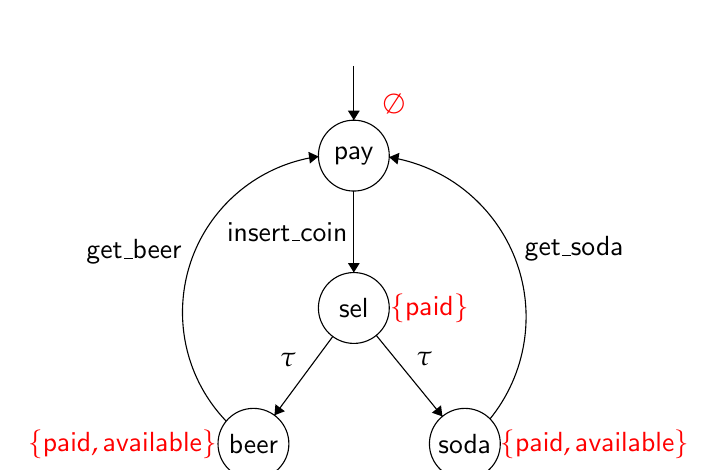
\begin{tikzpicture}[scale=0.15]
		\tikzstyle{every node}+=[inner sep=0pt]
		\draw [black] (38.6,-22.4) circle (3);
		\draw (38.6,-22.4) node {$\mathsf{pay}$};
		\draw [red] (42, -18) node {$\emptyset$};
		\draw [black] (38.6,-35.3) circle (3);
		\draw (38.6,-35.3) node {$\textsf{sel}$};
		\draw [red] (45, -35.3) node {$\{\textsf{paid}\}$};
		\draw [black] (30.1,-46.8) circle (3);
		\draw (30.1,-46.8) node {$\textsf{beer}$};
		\draw [red] (19, -46.8) node {$\{\textsf{paid}, \textsf{available}\}$};
		\draw [black] (48,-46.8) circle (3);
		\draw (48,-46.8) node {$\textsf{soda}$};
		\draw [red] (59, -46.8) node {$\{\textsf{paid}, \textsf{available}\}$};
		\draw [black] (38.6,-14.8) -- (38.6,-19.4);
		\fill [black] (38.6,-19.4) -- (39.1,-18.6) -- (38.1,-18.6);
		\draw [black] (38.6,-25.4) -- (38.6,-32.3);
		\fill [black] (38.6,-32.3) -- (39.1,-31.5) -- (38.1,-31.5);
		\draw (38.1,-28.85) node [left] {$\textsf{insert\_coin}$};
		\draw [black] (36.82,-37.71) -- (31.88,-44.39);
		\fill [black] (31.88,-44.39) -- (32.76,-44.04) -- (31.96,-43.45);
		\draw (33.77,-39.66) node [left] {$\tau$};
		\draw [black] (40.5,-37.62) -- (46.1,-44.48);
		\fill [black] (46.1,-44.48) -- (45.98,-43.54) -- (45.21,-44.17);
		\draw (43.86,-39.62) node [right] {$\tau$};
		\draw [black] (27.798,-44.886) arc (-136.20523:-262.20742:13.32);
		\fill [black] (35.61,-22.47) -- (34.75,-22.08) -- (34.88,-23.07);
		\draw (24.07,-30.54) node [left] {$\textsf{get\_beer}$};
		\draw [black] (41.591,-22.534) arc (81.15163:-39.01368:13.699);
		\fill [black] (41.59,-22.53) -- (42.3,-23.15) -- (42.46,-22.16);
		\draw (53.02,-30.3) node [right] {$\textsf{get\_soda}$};
		\end{tikzpicture}
	\end{center}
	The $\tau$ transitions are conventionally assumed to be non-deterministic from the point of view of the observer. The transition system depicted here has states $S = \{\textsf{pay}, \textsf{select}, \textsf{soda}, \textsf{beer}\}$, $A = \{\textsf{ic}, \textsf{gs}, \textsf{gb}\}$\footnote{It is common practice to assume that $\tau$ is an action.}, $I = \{\textsf{pay}\}$, $\AP = \{\textsf{paid}, \textsf{available}\}$ and $L$ assigns $\emptyset$ to $\textsf{pay}$, $\{\textsf{paid}\}$ to \textsf{sel}  and $\{\textsf{paid},  \textsf{available}\}$ to \textsf{soda} and \textsf{beer}.
\end{exmp}

In the context of this course, and especially for this section, it is useful to have a way to generate transition systems. \textbf{Program graphs}, although they are designed to represent the evaluation of a program, can do exactly this.

\begin{defn}[Program graph]\label{defn-pg}
	Given a (finite) set $\Vars$ of \textbf{variables} together with, for each variable $x \in \Vars$, a \textbf{domain} $\Dom(x)$\footnote{Example of such domains are lists, machine integers, $\Z$, $\R$. Note that they can be infinite and even contain stuff that cannot be represented by a computer. This is because it is sometimes useful to abstract away these restrictions.}, an \textbf{evaluation} is an element of $\Eval(\Vars) = \prod_{x \in \Vars} \Dom(x)$, that is, $\eta \in \Eval(\Vars)$ assigns a value $\eta(x) \in \Dom(x)$ to each variable $x \in \Vars$.\footnote{In other words, an evaluation can be viewed as the state of the memory at a specific point in the program.} We write $\Eval$ when the set of variables is clear from the context.
	
	%TODO: (i.e.: closed under conjunction, disjunction and negation) + examples
	A \textbf{condition} is a propositional formula with atoms of the form $x \in D$ where $x \in \Vars$ and $D \subseteq \Dom(x)$ or $\top$ and $\bot$ to represent true and false values respectively. The set of such conditions denoted $\Cond(\Vars)$ (or simply $\Cond$) is of course closed under conjunctions, disjunctions and negations. Given a condition $g \in \Cond$ and a valuation $\eta \in \Eval$, we write $\eta \vDash g$ if $g$ is true under the evaluation $\eta$.
	
	A \textbf{program graph} over $\Vars$ has the form $PG = (\Loc, A, \Eff, \hookrightarrow, \Loc_0, g_0)$, where:
	\begin{enumerate}
		\item $\Loc$ is the (usually fininte) set of locations\footnote{They are an abstraction of the line number in the code, or of labels in assembly, another terminology is control point.},
		\item $A$ is the set of actions,
		\item $\Eff: A \times \Eval \rightarrow \Eval$ abstracts the effect that actions have on memory,
		\item $\hookrightarrow\subseteq \Loc \times \Cond  \times A \times \Loc$ which is a transition relation guarded by a condition\footnote{ We will denote $\ell \action{g:a} \ell'$ when $(\ell, g, a, \ell') \in \hookrightarrow$. It roughly translates to \textquotedblleft If we are in location $\ell$ and condition $g$ is holds, then we can execute action $a$ apply its effects and go to location $\ell'$.\textquotedblright},
		\item $\Loc_0 \subseteq \Loc$ is the set of initial locations and $g_0 \in \Cond$ is the initial condition.
	\end{enumerate}
\end{defn}
\begin{exmp}[Vending machine (continued)]\label{exmp-vendingII}
	Let us extend Example \ref{exmp-vending} by giving the program graph for a vending machine with a similar behavior. The only difference is that there is a now a set amount of beers and sodas in the machine that can be refilled. When the user inserts a coin but there are no items left, the coin is returned.
	
	Fix the maximum number of items $m \in \N$, let the amount of beers and sodas be variables in $n_b, n_s \in \Vars$ with domain $\Dom(n_b) = \Dom(n_s) = \{0, \dots, max-1\}$. There are two control points $\Loc_0 = \textsf{start}, \textsf{sel} \in \Loc$ and new actions to refill and return the coin ($A = \{\textsf{ic}, \textsf{gb}, \textsf{gs}, \textsf{refill}, \textsf{rc}\}$). The initial condition is $g_0 = n_b = m-1 \wedge n_s = m-1$.

\begin{center}
	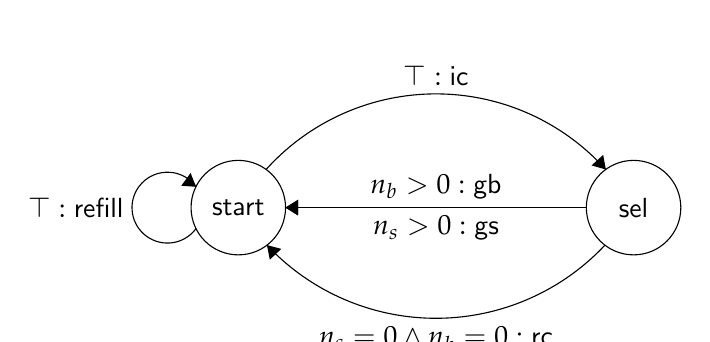
\begin{tikzpicture}[scale=0.2]
	\tikzstyle{every node}+=[inner sep=0pt]
	\draw [black] (21.1,-39.7) circle (3);
	\draw (21.1,-39.7) node {$\textsf{start}$};
	\draw [black] (46.2,-39.7) circle (3);
	\draw (46.2,-39.7) node {$\textsf{sel}$};
	\draw [black] (22.864,-37.28) arc (137.99491:42.00509:14.515);
	\fill [black] (44.44,-37.28) -- (44.27,-36.35) -- (43.53,-37.02);
	\draw (33.65,-31.98) node [above] {$\top:\textsf{ic}$};
	\draw [black] (44.383,-42.081) arc (-43.18694:-136.81306:14.721);
	\fill [black] (22.92,-42.08) -- (23.1,-43.01) -- (23.83,-42.32);
	\draw (33.65,-47.23) node [below] {$n_s=0\wedge n_b=0:\textsf{rc}$};
	\draw [black] (43.2,-39.7) -- (24.1,-39.7);
	\fill [black] (24.1,-39.7) -- (24.9,-40.2) -- (24.9,-39.2);
	\draw (33.65,-40.2) node [below] {$n_s>0:\textsf{gs}$};
	\draw [black] (18.42,-41.023) arc (-36:-324:2.25);
	\draw (13.85,-39.7) node [left] {$\top:\textsf{refill}$};
	\fill [black] (18.42,-38.38) -- (18.07,-37.5) -- (17.48,-38.31);
	\draw [black] (43.2,-39.7) -- (24.1,-39.7);
	\fill [black] (24.1,-39.7) -- (24.9,-40.2) -- (24.9,-39.2);
	\draw (33.65,-39.2) node [above] {$n_b>0:\textsf{gb}$};
	\end{tikzpicture}
\end{center}

The effects are not represented in the diagram but a sensible $\Eff$ would satisfy: for any evaluation $\eta \in \Eval$,
\begin{align*}
	\Eff(\eta, \textsf{ic}) = \Eff(\eta, \textsf{rc}) &= \eta\\
	\Eff(\eta, \textsf{gb}) &= \eta[n_b:=n_b-1]\\
	\Eff(\eta, \textsf{gs}) &= \eta[n_s:=n_s-1]\\
	\Eff(\eta, \textsf{refill}) &= \eta[n_b:=100, n_s:=100].
\end{align*}
\end{exmp}
The crucial difference between program graphs and transition systems is that the former separate the control from the data. In other words, a program graph abstracts only the behavior the program while a transition system abstracts the behavior along with the memory of the program. This motivates that a transition system might be more appropriate for observing the evolution of a program graph along with the evaluation. The following definition makes this formal.
\begin{defn}[TS of a PG]
	Let us have a program graph $PG$ with the same notation as in Definition \ref{defn-pg}, the transition system of $PG$ is $TS(PG) = (\Loc \times \Eval, A, \rightarrow, I, \AP, L)$\footnote{Note that this can lead to a huge set of states because some variables can have huge domains.}, where:
	\begin{enumerate}
		\item $\rightarrow$ is defined by the rule 
		\[	\begin{bprooftree}
				\AxiomC{$\ell \action{g: \alpha} \ell'$}
				\AxiomC{$n\vDash g$}
				\RightLabel{}
				\BinaryInfC{$(\ell, \eta) \stackrel{\alpha}{\rightarrow} (\ell', \Eff(\eta, \alpha))$}
			\end{bprooftree},\] 
		\item $I = \{(\ell, \eta)\mid \ell \in Loc_0, \eta \vDash g_0\}$,\footnote{We require that the initial condition is satisfied with $\eta$ in memory.}
		\item $\AP = \Loc + \Cond(\Vars)$,\footnote{In words, the atomic properties can say whether a state is in a certain location or whether it satisfies a condition of $\Cond$. In practice, we use a smaller subset of $\AP$ that contains only properties relevant to the particular application.}
		\item $L(\ell, \eta) = \{\ell\} \cup \{g \mid \eta \vDash g\}$.
	\end{enumerate}
\end{defn}
\begin{exmp}[Vending machine (still)]
	Assuming that the $m=2$, we can draw the transition graph for the vending machine in Example \ref{exmp-vendingII} (we omit the state labeling as it is clear what properties hold at each state). We denote the evaluations as a pairs of values $(n_s,n_b)$.
	\begin{center}
		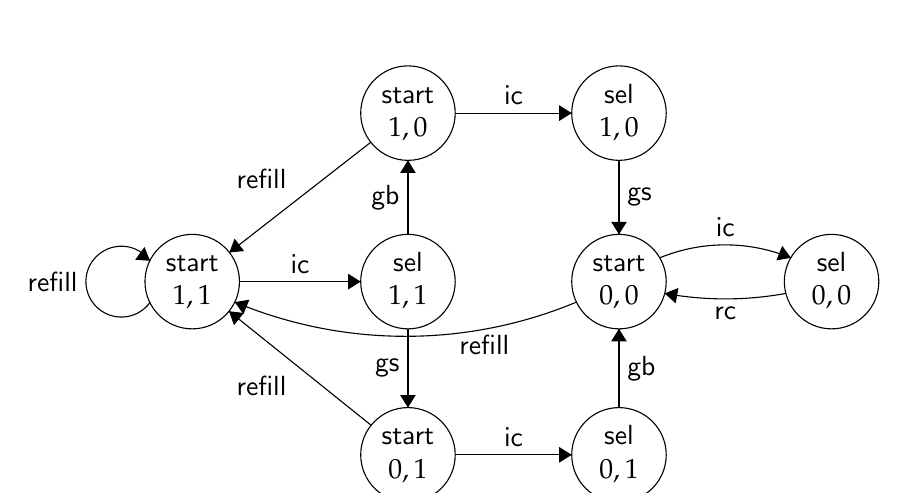
\begin{tikzpicture}[scale=0.2]
		\tikzstyle{every node}+=[inner sep=0pt]
		\draw [black] (20,-28.1) circle (3);
		\draw (20,-28.1) node {$\begin{matrix}\textsf{start}\\1,1\end{matrix}$};
		\draw [black] (33.7,-28.1) circle (3);
		\draw (33.7,-28.1) node {$\begin{matrix}\textsf{sel}\\1,1\end{matrix}$};
		\draw [black] (33.7,-17.4) circle (3);
		\draw (33.7,-17.4) node {$\begin{matrix}\textsf{start}\\1,0\end{matrix}$};
		\draw [black] (33.7,-39.1) circle (3);
		\draw (33.7,-39.1) node {$\begin{matrix}\textsf{start}\\0,1\end{matrix}$};
		\draw [black] (47.1,-17.4) circle (3);
		\draw (47.1,-17.4) node {$\begin{matrix}\textsf{sel}\\1,0\end{matrix}$};
		\draw [black] (47.1,-39.1) circle (3);
		\draw (47.1,-39.1) node {$\begin{matrix}\textsf{sel}\\0,1\end{matrix}$};
		\draw [black] (47.1,-28.1) circle (3);
		\draw (47.1,-28.1) node {$\begin{matrix}\textsf{start}\\0,0\end{matrix}$};
		\draw [black] (60.6,-28.1) circle (3);
		\draw (60.6,-28.1) node {$\begin{matrix}\textsf{sel}\\0,0\end{matrix}$};
		\draw [black] (17.32,-29.423) arc (-36:-324:2.25);
		\draw (12.75,-28.1) node [left] {$\textsf{refill}$};
		\fill [black] (17.32,-26.78) -- (16.97,-25.9) -- (16.38,-26.71);
		\draw [black] (23,-28.1) -- (30.7,-28.1);
		\fill [black] (30.7,-28.1) -- (29.9,-27.6) -- (29.9,-28.6);
		\draw (26.85,-27.6) node [above] {$\textsf{ic}$};
		\draw [black] (33.7,-25.1) -- (33.7,-20.4);
		\fill [black] (33.7,-20.4) -- (33.2,-21.2) -- (34.2,-21.2);
		\draw (33.2,-22.75) node [left] {$\textsf{gb}$};
		\draw [black] (33.7,-31.1) -- (33.7,-36.1);
		\fill [black] (33.7,-36.1) -- (34.2,-35.3) -- (33.2,-35.3);
		\draw (33.2,-33.6) node [left] {$\textsf{gs}$};
		\draw [black] (36.7,-17.4) -- (44.1,-17.4);
		\fill [black] (44.1,-17.4) -- (43.3,-16.9) -- (43.3,-17.9);
		\draw (40.4,-16.9) node [above] {$\textsf{ic}$};
		\draw [black] (36.7,-39.1) -- (44.1,-39.1);
		\fill [black] (44.1,-39.1) -- (43.3,-38.6) -- (43.3,-39.6);
		\draw (40.4,-38.6) node [above] {$\textsf{ic}$};
		\draw [black] (47.1,-20.4) -- (47.1,-25.1);
		\fill [black] (47.1,-25.1) -- (47.6,-24.3) -- (46.6,-24.3);
		\draw (47.6,-22.75) node [right] {$\textsf{gs}$};
		\draw [black] (47.1,-36.1) -- (47.1,-31.1);
		\fill [black] (47.1,-31.1) -- (46.6,-31.9) -- (47.6,-31.9);
		\draw (47.6,-33.6) node [right] {$\textsf{gb}$};
		\draw [black] (49.683,-26.592) arc (112.40996:67.59004:10.931);
		\fill [black] (58.02,-26.59) -- (57.47,-25.83) -- (57.09,-26.75);
		\draw (53.85,-25.27) node [above] {$\textsf{ic}$};
		\draw [black] (57.697,-28.848) arc (-79.58325:-100.41675:21.279);
		\fill [black] (50,-28.85) -- (50.7,-29.48) -- (50.88,-28.5);
		\draw (53.85,-29.7) node [below] {$\textsf{rc}$};
		\draw [black] (31.34,-19.25) -- (22.36,-26.25);
		\fill [black] (22.36,-26.25) -- (23.3,-26.16) -- (22.69,-25.37);
		\draw (24.4,-22.25) node [above] {$\textsf{refill}$};
		\draw [black] (31.36,-37.22) -- (22.34,-29.98);
		\fill [black] (22.34,-29.98) -- (22.65,-30.87) -- (23.28,-30.09);
		\draw (24.4,-34.09) node [below] {$\textsf{refill}$};
		\draw [black] (44.398,-29.401) arc (-67.34371:-112.65629:28.162);
		\fill [black] (22.7,-29.4) -- (23.25,-30.17) -- (23.63,-29.25);
		\draw (38.55,-31.5) node [below] {$\textsf{refill}$};
		\end{tikzpicture}
	\end{center}
	Notice that increasing $m$, even by only one, would make the transition graph way more complex.
\end{exmp}

%TODO: motivation
%The important takeaway is the two levels of abstractions for th, where we want to talk about properties (the tranisition systems) and program graphs are just a way to generate transition systems.
%The methods of automatic verification, in fine, are based on exhaustive states exploration. There are also semi-automatic verification which requires the human to model the program as a transition system that abstracts more efficiently the data (to remove all states that depend on what values can take). In other words, it is more useful to analyze control-driven program compared to data-driven program.  Resolving concurrencies in parallel systems but not numerically-sensible computations.

To end this section presenting the basics of transition systems, we describe three ways of combining them.

The first one is similar to taking the product of two DFA\footnote{Deterministic finite automata.}, but we allow the case where some system can do an action that the other cannot. \footnote{In DFA terminology, it amounts to taking the products of two automata on different alphabets. When the new machine sees a letter that only one of the original DFA recognizes, it makes a transition only according to that DFA. When it sees a letter that both DFA recognize, it non-deterministically choose what transition to make. There is a slight caveat because actions are not consumed by a transition system, so after doing a common action on one of the system, the new machine can still do that action on the other system.}
\begin{defn}[Interleaving of TSs]
	Given two transition systems $T_i = (S_i, A_i, \rightarrow_i, I_i, \AP_i, L_i)$ for $i=1,2$, their interleaving composition denoted $T_1 \tmid T_2$ is $(S_1 \times S_2, A_1 \cup A_2, \rightarrow, I_1 \times I_2, \AP_1 \cup \AP_2, L)$, where $\rightarrow$ is defined by 
	\[\begin{bprooftree}
		\AxiomC{$s_1 \action{\alpha}_1 s_1'$}
		\RightLabel{}
		\UnaryInfC{$(s_1, s_2)\action{\alpha}(s_1', s_2)$}
	\end{bprooftree} \quad \begin{bprooftree}
	\AxiomC{$s_2 \action{\alpha}_2 s_2'$}
	\RightLabel{}
	\UnaryInfC{$(s_1, s_2)\action{\alpha}(s_1, s_2')$}
	\end{bprooftree},\]
	and $L(s_1, s_2) =  L_1(s_1) \cup L_2(s_2)$.
\end{defn}
\begin{exmp}[Traffic lights]
	Suppose we have two traffic lights with that can switch from red to green and vice-versa non-deterministically, they are represented by the following graphs.
	\begin{center}
		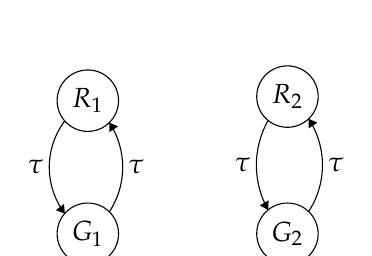
\begin{tikzpicture}[scale=0.13]
		\tikzstyle{every node}+=[inner sep=0pt]
		\draw [black] (14.5,-11.2) circle (3);
		\draw (14.5,-11.2) node {$R_1$};
		\draw [black] (14.5,-24.2) circle (3);
		\draw (14.5,-24.2) node {$G_1$};
		\draw [black] (34,-10.8) circle (3);
		\draw (34,-10.8) node {$R_2$};
		\draw [black] (34,-24.2) circle (3);
		\draw (34,-24.2) node {$G_2$};
		\draw [black] (12.261,-22.234) arc (-142.75626:-217.24374:7.491);
		\fill [black] (12.26,-22.23) -- (12.17,-21.29) -- (11.38,-21.9);
		\draw (10.23,-17.7) node [left] {$\tau$};
		\draw [black] (16.589,-13.328) arc (33.58261:-33.58261:7.903);
		\fill [black] (16.59,-13.33) -- (16.61,-14.27) -- (17.45,-13.72);
		\draw (18.41,-17.7) node [right] {$\tau$};
		\draw [black] (32.117,-21.883) arc (-150.53579:-209.46421:8.911);
		\fill [black] (32.12,-21.88) -- (32.16,-20.94) -- (31.29,-21.43);
		\draw (30.46,-17.5) node [left] {$\tau$};
		\draw [black] (36.062,-12.957) arc (33.31849:-33.31849:8.271);
		\fill [black] (36.06,-12.96) -- (36.08,-13.9) -- (36.92,-13.35);
		\draw (37.92,-17.5) node [right] {$\tau$};
		\end{tikzpicture}
	\end{center}
	Taking their interleaving yields the following transition system.\footnote{We left out the state labeling as it is a trivial construction.}
	\begin{center}
		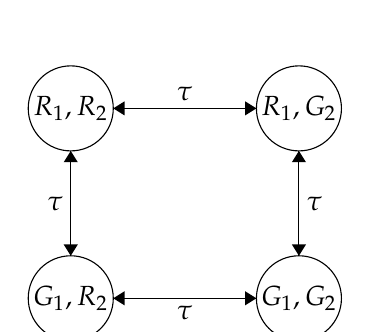
\begin{tikzpicture}[scale=0.18]
		\tikzstyle{every node}+=[inner sep=0pt]
		\draw [black] (44.2,-18) circle (3);
		\draw (44.2,-18) node {$R_1,G_2$};
		\draw [black] (28.1,-18) circle (3);
		\draw (28.1,-18) node {$R_1,R_2$};
		\draw [black] (28.1,-31.4) circle (3);
		\draw (28.1,-31.4) node {$G_1,R_2$};
		\draw [black] (44.2,-31.4) circle (3);
		\draw (44.2,-31.4) node {$G_1,G_2$};
		\draw [black] (28.1,-21) -- (28.1,-28.4);
		\fill [black] (28.1,-28.4) -- (28.6,-27.6) -- (27.6,-27.6);
		\draw [black] (28.1,-28.4) -- (28.1,-21);
		\fill [black] (28.1,-21) -- (27.6,-21.8) -- (28.6,-21.8);
		\draw (27.6,-24.7) node [left] {$\tau$};
		\draw [black] (31.1,-31.4) -- (41.2,-31.4);
		\fill [black] (41.2,-31.4) -- (40.4,-30.9) -- (40.4,-31.9);
		\draw (36.15,-31.9) node [below] {$\tau$};
		\draw [black] (41.2,-31.4) -- (31.1,-31.4);
		\fill [black] (31.1,-31.4) -- (31.9,-31.9) -- (31.9,-30.9);
		\draw [black] (44.2,-28.4) -- (44.2,-21);
		\fill [black] (44.2,-21) -- (43.7,-21.8) -- (44.7,-21.8);
		\draw (44.7,-24.7) node [right] {$\tau$};
		\draw [black] (44.2,-21) -- (44.2,-28.4);
		\fill [black] (44.2,-28.4) -- (44.7,-27.6) -- (43.7,-27.6);
		\draw [black] (41.2,-18) -- (31.1,-18);
		\fill [black] (31.1,-18) -- (31.9,-18.5) -- (31.9,-17.5);
		\draw (36.15,-17.5) node [above] {$\tau$};
		\draw [black] (31.1,-18) -- (41.2,-18);
		\fill [black] (41.2,-18) -- (40.4,-17.5) -- (40.4,-18.5);
		\end{tikzpicture}
	\end{center}

\end{exmp}

Unfortunately, such a simple way of composing transition systems does not allow shared memory between the systems. For this reason, when we want to take this possibility into account, it is preferred to do a composition of program graphs. 

\begin{defn}[Interleaving of PGs]
	Given two program graphs $G_i = (\Loc_i, A_i, \Eff_i, \hookrightarrow_i, \Loc_{i,0}, g_{i,0})$ over $\Vars_i$ for $i=1,2$, their interleaving is the program graph\footnote{Observe that the variables are not necessarily disjoint, hence we must consider actions of $A_1$ and $A_2$ as disjoint, otherwise there would be an ambiguity in the choice of what effect to apply.} over $\Vars_1 \cup \Vars_2$ denoted $G_1 \tmid G_2 = (\Loc_1 \times \Loc_2, A_1 + A_2, \Eff, \hookrightarrow, \Loc_{1,0} \times Loc_{2,0}, g_{1,0} \wedge g_{2,0})$, where $\hookrightarrow$ is defined by the rule 
	\[\begin{bprooftree}
	\AxiomC{$\ell_1 \action{g:\alpha}_1 \ell_1'$}
	\RightLabel{}
	\UnaryInfC{$(\ell_1, \ell_2)\action{g:\alpha}(\ell_1', \ell_2)$}
	\end{bprooftree} \quad \begin{bprooftree}
	\AxiomC{$\ell_2 \action{g:\alpha}_2 \ell_2'$}
	\RightLabel{}
	\UnaryInfC{$(\ell_1, \ell_2)\action{\alpha}(\ell_1, \ell_2')$}
	\end{bprooftree},\]
	and 
	$\Eff(\alpha, \eta) = \Eff_i(\alpha ,\eta)$ for $\alpha \in A_i$.\footnote{The evaluation $\eta$ is an element of $\Eval(\Vars_1 \cup \Vars_2)$, so we implicitly adapted $\Eff_i$ in the obvious way (i.e.: it does not modify variables outside $\Vars_i$).}
\end{defn}
\begin{exmp}\label{exmp-interpg}
	Let us illustrate this construction on two simple program graphs manipulating the same variable $x$ with $\Dom(x) = \N$, here are their representations with effects in blue. 
	\begin{center}
		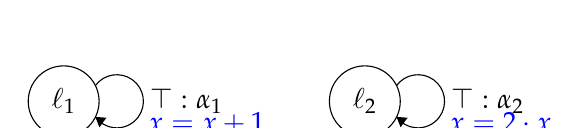
\begin{tikzpicture}[scale=0.15]
		\tikzstyle{every node}+=[inner sep=0pt]
		\draw [black] (28.1,-31.4) circle (3);
		\draw (28.1,-31.4) node {$\ell_1$};
		\draw [black] (53.6,-31.4) circle (3);
		\draw (53.6,-31.4) node {$\ell_2$};
		\draw [black] (30.78,-30.077) arc (144:-144:2.25);
		\draw (35.35,-31.4) node [right] {$\top:\alpha_1$};
		\draw [blue] (35.2,-33.2) node [right] {$x= x+1$};
		\fill [black] (30.78,-32.72) -- (31.13,-33.6) -- (31.72,-32.79);
		\draw [black] (56.28,-30.077) arc (144:-144:2.25);
		\draw (60.85,-31.4) node [right] {$\top:\alpha_2$};
		\draw [blue] (60.7,-33.2) node [right] {$x=2\cdot x$};
		\fill [black] (56.28,-32.72) -- (56.63,-33.6) -- (57.22,-32.79);
		\end{tikzpicture}
	\end{center}
	\begin{marginfigure}
		\begin{center}
			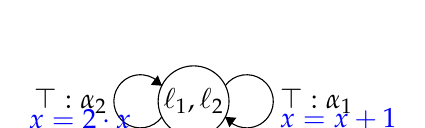
\begin{tikzpicture}[scale=0.15]
			\tikzstyle{every node}+=[inner sep=0pt]
			\draw [black] (38.5,-27.8) circle (3);
			\draw (38.5,-27.8) node {$\ell_1,\ell_2$};
			\draw [black] (41.18,-26.477) arc (144:-144:2.25);
			\draw (45.75,-27.8) node [right] {$\top:\alpha_1$};
			\draw [blue] (45.75,-29.3) node [right] {$x=x+1$};
			\fill [black] (41.18,-29.12) -- (41.53,-30) -- (42.12,-29.19);
			\draw [black] (35.82,-29.123) arc (-36:-324:2.25);
			\draw (31.25,-27.8) node [left] {$\top:\alpha_2$};
			\draw [blue] (24.5,-29.3) node [right] {$x=2\cdot x$};
			\fill [black] (35.82,-26.48) -- (35.47,-25.6) -- (34.88,-26.41);
			\end{tikzpicture}
		\end{center}
		\caption{Interleaving of program graphs in Example \ref{exmp-interpg}.}\label{fig-simplepg}
	\end{marginfigure}
	Interleaving the program graphs is simple enough (see Figure \ref{fig-simplepg}), but what is more interesting is comparing the transition systems we obtain when do the operations $TS(G_1) \tmid TS(G_2)$ and $TS(G_1 \tmid G_2)$. Since the domain of $x$ is infinite, both these transition systems have infinitely many states.
	
	\begin{marginfigure}
		\begin{center}
			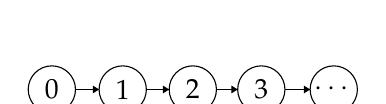
\begin{tikzpicture}[scale=0.1]
			\tikzstyle{every node}+=[inner sep=0pt]
			\draw [black] (7.6,-30) circle (3);
			\draw (7.6,-30) node {$0$};
			\draw [black] (16.6,-30) circle (3);
			\draw (16.6,-30) node {$1$};
			\draw [black] (25.5,-30) circle (3);
			\draw (25.5,-30) node {$2$};
			\draw [black] (34.2,-30) circle (3);
			\draw (34.2,-30) node {$3$};
			\draw [black] (43.4,-30) circle (3);
			\draw (43.4,-30) node {$\cdots$};
			\draw [black] (10.6,-30) -- (13.6,-30);
			\fill [black] (13.6,-30) -- (12.8,-29.5) -- (12.8,-30.5);
			\draw [black] (19.6,-30) -- (22.5,-30);
			\fill [black] (22.5,-30) -- (21.7,-29.5) -- (21.7,-30.5);
			\draw [black] (28.5,-30) -- (31.2,-30);
			\fill [black] (31.2,-30) -- (30.4,-29.5) -- (30.4,-30.5);
			\draw [black] (37.2,-30) -- (40.4,-30);
			\fill [black] (40.4,-30) -- (39.6,-29.5) -- (39.6,-30.5);
			\end{tikzpicture}
		\end{center}
		\begin{center}
			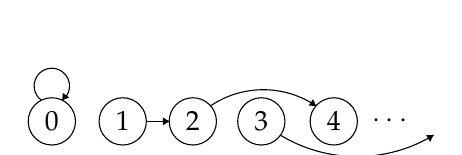
\begin{tikzpicture}[scale=0.1]
			\tikzstyle{every node}+=[inner sep=0pt]
			\draw [black] (7.6,-30) circle (3);
			\draw (7.6,-30) node {$0$};
			\draw [black] (16.6,-30) circle (3);
			\draw (16.6,-30) node {$1$};
			\draw [black] (25.5,-30) circle (3);
			\draw (25.5,-30) node {$2$};
			\draw [black] (34.2,-30) circle (3);
			\draw (34.2,-30) node {$3$};
			\draw [black] (43.4,-30) circle (3);
			\draw (43.4,-30) node {$4$};
			\draw (50.8,-30) node {$\cdots$};
			\draw [black] (19.6,-30) -- (22.5,-30);
			\fill [black] (22.5,-30) -- (21.7,-29.5) -- (21.7,-30.5);
			\draw [black] (6.277,-27.32) arc (234:-54:2.25);
			\fill [black] (8.92,-27.32) -- (9.8,-26.97) -- (8.99,-26.38);
			\draw [black] (27.751,-28.028) arc (124.03543:55.96457:11.969);
			\fill [black] (41.15,-28.03) -- (40.77,-27.17) -- (40.21,-28);
			\draw [black] (56.069,-31.753) arc (-58.78348:-121.21652:18.753);			
			\fill [black] (56.07,-31.75) -- (55.13,-31.74) -- (55.64,-32.6);
			\end{tikzpicture}
		\end{center}
		\caption{Part of $TS(G_1)$ and $TS(G_2)$ from Example \ref{exmp-interpg}. (the label of the nodes is the value of $x$ at that state)}\label{fig-simpletspg}
	\end{marginfigure}
	For the former, observe that interleaving $TS(G_1)$ and $TS(G_2)$ (represented in Figure \ref{fig-simpletspg}) will lead to the dissociation of the variable $x$ into two independent copies. It leads to a system (partially represented below) which is irrelevant for the purpose of analyzing the behavior of both programs when run concurrently.
	\begin{center}
		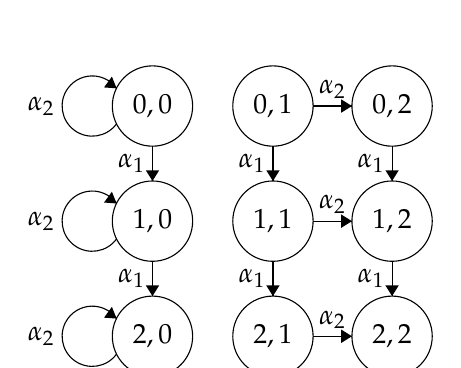
\begin{tikzpicture}[scale=0.17]
		\tikzstyle{every node}+=[inner sep=0pt]
		\draw [black] (7.6,-30) circle (3);
		\draw (7.6,-30) node {$0,0$};
		\draw [black] (16.6,-30) circle (3);
		\draw (16.6,-30) node {$0,1$};
		\draw [black] (25.5,-30) circle (3);
		\draw (25.5,-30) node {$0,2$};
		\draw [black] (7.6,-38.6) circle (3);
		\draw (7.6,-38.6) node {$1,0$};
		\draw [black] (16.6,-38.6) circle (3);
		\draw (16.6,-38.6) node {$1,1$};
		\draw [black] (25.5,-38.6) circle (3);
		\draw (25.5,-38.6) node {$1,2$};
		\draw [black] (7.6,-47.2) circle (3);
		\draw (7.6,-47.2) node {$2,0$};
		\draw [black] (16.6,-47.2) circle (3);
		\draw (16.6,-47.2) node {$2,1$};
		\draw [black] (25.5,-47.2) circle (3);
		\draw (25.5,-47.2) node {$2,2$};
		\draw [black] (19.6,-30) -- (22.5,-30);
		\fill [black] (22.5,-30) -- (21.7,-29.5) -- (21.7,-30.5);
		\draw (21.05,-29.5) node [above] {$\alpha_2$};
		\draw [black] (4.92,-31.323) arc (-36:-324:2.25);
		\draw (0.35,-30) node [left] {$\alpha_2$};
		\fill [black] (4.92,-28.68) -- (4.57,-27.8) -- (3.98,-28.61);
		\draw [black] (7.6,-33) -- (7.6,-35.6);
		\fill [black] (7.6,-35.6) -- (8.1,-34.8) -- (7.1,-34.8);
		\draw (7.1,-34.3) node [left] {$\alpha_1$};
		\draw [black] (7.6,-41.6) -- (7.6,-44.2);
		\fill [black] (7.6,-44.2) -- (8.1,-43.4) -- (7.1,-43.4);
		\draw (7.1,-42.9) node [left] {$\alpha_1$};
		\draw [black] (16.6,-33) -- (16.6,-35.6);
		\fill [black] (16.6,-35.6) -- (17.1,-34.8) -- (16.1,-34.8);
		\draw (16.1,-34.3) node [left] {$\alpha_1$};
		\draw [black] (16.6,-41.6) -- (16.6,-44.2);
		\fill [black] (16.6,-44.2) -- (17.1,-43.4) -- (16.1,-43.4);
		\draw (16.1,-42.9) node [left] {$\alpha_1$};
		\draw [black] (25.5,-33) -- (25.5,-35.6);
		\fill [black] (25.5,-35.6) -- (26,-34.8) -- (25,-34.8);
		\draw (25,-34.3) node [left] {$\alpha_1$};
		\draw [black] (25.5,-41.6) -- (25.5,-44.2);
		\fill [black] (25.5,-44.2) -- (26,-43.4) -- (25,-43.4);
		\draw (25,-42.9) node [left] {$\alpha_1$};
		\draw [black] (19.6,-38.6) -- (22.5,-38.6);
		\fill [black] (22.5,-38.6) -- (21.7,-38.1) -- (21.7,-39.1);
		\draw (21.05,-38.1) node [above] {$\alpha_2$};
		\draw [black] (19.6,-47.2) -- (22.5,-47.2);
		\fill [black] (22.5,-47.2) -- (21.7,-46.7) -- (21.7,-47.7);
		\draw (21.05,-46.7) node [above] {$\alpha_2$};
		\draw [black] (4.92,-39.923) arc (-36:-324:2.25);
		\draw (0.35,-38.6) node [left] {$\alpha_2$};
		\fill [black] (4.92,-37.28) -- (4.57,-36.4) -- (3.98,-37.21);
		\draw [black] (4.92,-48.523) arc (-36:-324:2.25);
		\draw (0.35,-47.2) node [left] {$\alpha_2$};
		\fill [black] (4.92,-45.88) -- (4.57,-45) -- (3.98,-45.81);
		\end{tikzpicture}
	\end{center}
	For the latter, we actually obtain an interesting system (depicted below) because interleaving the program graphs first ensures that $\alpha_1$ and $\alpha_2$ act on the same $x$.
	\begin{center}
		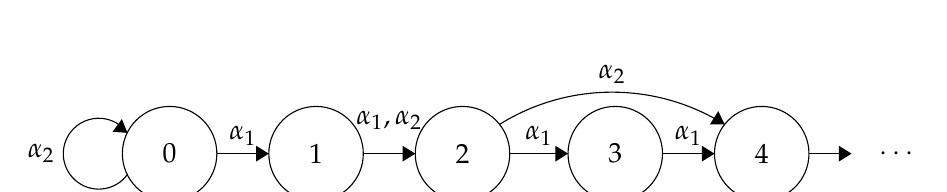
\begin{tikzpicture}[scale=0.2]
		\tikzstyle{every node}+=[inner sep=0pt]
		\draw [black] (7.6,-30) circle (3);
		\draw (7.6,-30) node {$0$};
		\draw [black] (16.9,-30) circle (3);
		\draw (16.9,-30) node {$1$};
		\draw [black] (26.2,-30) circle (3);
		\draw (26.2,-30) node {$2$};
		\draw [black] (35.9,-30) circle (3);
		\draw (35.9,-30) node {$3$};
		\draw [black] (45.2,-30) circle (3);
		\draw (45.2,-30) node {$4$};
		\draw (53.9,-30) node {$\cdots$};
		\draw [black] (19.9,-30) -- (23.2,-30);
		\fill [black] (23.2,-30) -- (22.4,-29.5) -- (22.4,-30.5);
		\draw (21.55,-28.5) node [above] {$\alpha_1,\alpha_2$};
		\draw [black] (4.92,-31.323) arc (-36:-324:2.25);
		\draw (0.35,-30) node [left] {$\alpha_2$};
		\fill [black] (4.92,-28.68) -- (4.57,-27.8) -- (3.98,-28.61);
		\draw [black] (10.6,-30) -- (13.9,-30);
		\fill [black] (13.9,-30) -- (13.1,-29.5) -- (13.1,-30.5);
		\draw (12.25,-29.5) node [above] {$\alpha_1$};
		\draw [black] (29.2,-30) -- (32.9,-30);
		\fill [black] (32.9,-30) -- (32.1,-29.5) -- (32.1,-30.5);
		\draw (31.05,-29.5) node [above] {$\alpha_1$};
		\draw [black] (38.9,-30) -- (42.2,-30);
		\fill [black] (42.2,-30) -- (41.4,-29.5) -- (41.4,-30.5);
		\draw (40.55,-29.5) node [above] {$\alpha_1$};
		\draw [black] (28.548,-28.143) arc (121.97321:58.02679:13.506);
		\fill [black] (42.85,-28.14) -- (42.44,-27.3) -- (41.91,-28.14);
		\draw (35.7,-25.59) node [above] {$\alpha_2$};
		\draw [black] (48.2,-30) -- (50.9,-30);
		\fill [black] (50.9,-30) -- (50.1,-29.5) -- (50.1,-30.5);
		\end{tikzpicture}
	\end{center}	
\end{exmp}
This example shows the relevance of program graphs when we care about concurrent data. While there are many more possibilities to compose transition systems, we introduce one last definition that illustrates how we can deal with concurrent control without using program graphs.

\begin{defn}[Parallel Composition of TSs]
	Let $T_i = (S_i, A_i, \rightarrow_i, I_i, \AP_i, L_i)$ for $i=1,2$ be two transition systems and $H \subseteq A_1\cap A_2$,\footnote{In general, we suppose $\tau \notin H$ and we write $T_1 \dmid T_2$ when $H = (A_1 \cap A_2)\setminus \{\tau\}$.} their \textbf{parallel composition} (or \textbf{handshaking}) is $T_1 \dmid_H T_2 = (S_1 \times S_2, A_1 \cup A_2, \rightarrow, I_1 \times I_2, \AP_1 \cup \AP_2, L)$, where $\rightarrow$ is defined by the rules
	\begin{gather*}
	\begin{bprooftree}
	\AxiomC{$s_1 \action{\alpha}_1 s_1'$}
	\AxiomC{$\alpha \notin H$}
	\RightLabel{}
	\BinaryInfC{$(s_1, s_2)\action{\alpha}(s_1', s_2)$}
	\end{bprooftree} \quad \begin{bprooftree}
	\AxiomC{$s_2 \action{\alpha}_2 s_2'$}
	\AxiomC{$\alpha \notin H$}
	\RightLabel{}
	\BinaryInfC{$(s_1, s_2)\action{\alpha}(s_1, s_2')$}
	\end{bprooftree}\\
	\begin{bprooftree}
	\AxiomC{$s_1 \action{\alpha}_1 s_1'$}
	\AxiomC{$s_2 \action{\alpha}_2 s_2'$}
	\AxiomC{$\alpha \in H$}
	\RightLabel{}
	\TrinaryInfC{$(s_1, s_2)\action{\alpha}(s_1', s_2')$}
	\end{bprooftree},
	\end{gather*}
	and $L(s_1, s_2) =  L_1(s_1) \cup L_2(s_2)$. One should view the actions in $H$ as \textit{synchronized} actions that both systems have to do at the same time.\footnote{Note that this definition is a generalization of the interleaving composition as $T_1 \dmid_{\emptyset} T_2 = T_1 \tmid T_2$.}
\end{defn}

\begin{exmp}\label{exmp-handshake}
	Given two transition systems $T_1$ and $T_2$ that have a non-critical state denoted $\textsf{nc}_i$ and a critical state $\textsf{c}_i$ and can jump from one to the other using actions $\textsf{req}$ and $\textsf{rel}$ as depicted below.\footnote{}%TODO:This example models two processes that are working with a shared memory and they should not be allowed to be  but that can do other calculations while the o.} Mutual exclusion. Show transitivity.
	
	
	\begin{center}
		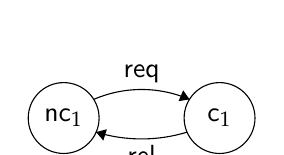
\begin{tikzpicture}[scale=0.15]
		\tikzstyle{every node}+=[inner sep=0pt]
		\draw [black] (22.3,-22.8) circle (3);
		\draw (22.3,-22.8) node {$\textsf{nc}_1$};
		\draw [black] (35.5,-22.8) circle (3);
		\draw (35.5,-22.8) node {$\textsf{c}_1$};
		\draw [black] (24.84,-21.224) arc (113.39952:66.60048:10.222);
		\fill [black] (32.96,-21.22) -- (32.42,-20.45) -- (32.03,-21.37);
		\draw (28.9,-19.88) node [above] {$\textsf{req}$};
		\draw [black] (32.755,-23.994) arc (-73.00767:-106.99233:13.191);
		\fill [black] (25.05,-23.99) -- (25.66,-24.71) -- (25.96,-23.75);
		\draw (28.9,-25.07) node [below] {$\textsf{rel}$};
		\end{tikzpicture}\quad
		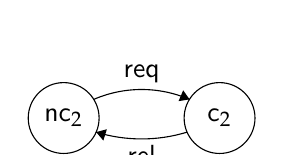
\begin{tikzpicture}[scale=0.15]
		\tikzstyle{every node}+=[inner sep=0pt]
		\draw [black] (22.3,-22.8) circle (3);
		\draw (22.3,-22.8) node {$\textsf{nc}_2$};
		\draw [black] (35.5,-22.8) circle (3);
		\draw (35.5,-22.8) node {$\textsf{c}_2$};
		\draw [black] (24.84,-21.224) arc (113.39952:66.60048:10.222);
		\fill [black] (32.96,-21.22) -- (32.42,-20.45) -- (32.03,-21.37);
		\draw (28.9,-19.88) node [above] {$\textsf{req}$};
		\draw [black] (32.755,-23.994) arc (-73.00767:-106.99233:13.191);
		\fill [black] (25.05,-23.99) -- (25.66,-24.71) -- (25.96,-23.75);
		\draw (28.9,-25.07) node [below] {$\textsf{rel}$};
		\end{tikzpicture}
	\end{center}
	
	We leave it as an exercise to show that in the plain interleaving composition of $T_1$ and $T_2$, both processes can reach their critical state at the same time. However, if we add an arbiter system $A$ that can unlock or lock the critical section, we can disallow this behavior: with $A$ is as in Figure \ref{fig-arbiter}, $A \dmid_{\textsf{rel}, \textsf{req}} (T_1 \tmid T_2)$ is as follows.
	\begin{marginfigure}
		\begin{center}
			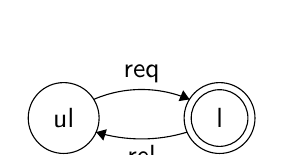
\begin{tikzpicture}[scale=0.15]
			\tikzstyle{every node}+=[inner sep=0pt]
			\draw [black] (22.3,-22.8) circle (3);
			\draw (22.3,-22.8) node {$\textsf{ul}$};
			\draw [black] (35.5,-22.8) circle (3);
			\draw [black] (35.5,-22.8) circle (2.4);
			\draw (35.5,-22.8) node {$\textsf{l}$};
			\draw [black] (24.84,-21.224) arc (113.39952:66.60048:10.222);
			\fill [black] (32.96,-21.22) -- (32.42,-20.45) -- (32.03,-21.37);
			\draw (28.9,-19.88) node [above] {$\textsf{req}$};
			\draw [black] (32.755,-23.994) arc (-73.00767:-106.99233:13.191);
			\fill [black] (25.05,-23.99) -- (25.66,-24.71) -- (25.96,-23.75);
			\draw (28.9,-25.07) node [below] {$\textsf{rel}$};
			\end{tikzpicture}
		\end{center}
		\caption{Arbiter system in Example \ref{exmp-handshake}.}\label{fig-arbiter}
	\end{marginfigure}
	\begin{center}
		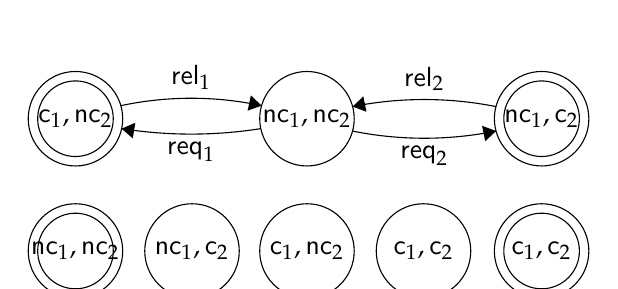
\begin{tikzpicture}[scale=0.2]
		\tikzstyle{every node}+=[inner sep=0pt]
		\draw [black] (25.4,-22.8) circle (3);
		\draw (25.4,-22.8) node {$\textsf{nc}_1,\textsf{nc}_2$};
		\draw [black] (25.4,-31.2) circle (3);
		\draw (25.4,-31.2) node {$\textsf{c}_1,\textsf{nc}_2$};
		\draw [black] (18.1,-31.2) circle (3);
		\draw (18.1,-31.2) node {$\textsf{nc}_1,\textsf{c}_2$};
		\draw [black] (32.8,-31.2) circle (3);
		\draw (32.8,-31.2) node {$\textsf{c}_1,\textsf{c}_2$};
		\draw [black] (10.7,-31.2) circle (3);
		\draw (10.7,-31.2) node {$\textsf{nc}_1,\textsf{nc}_2$};
		\draw [black] (10.7,-31.2) circle (2.4);
		\draw [black] (10.7,-22.8) circle (3);
		\draw (10.7,-22.8) node {$\textsf{c}_1,\textsf{nc}_2$};
		\draw [black] (10.7,-22.8) circle (2.4);
		\draw [black] (40.3,-22.8) circle (3);
		\draw (40.3,-22.8) node {$\textsf{nc}_1,\textsf{c}_2$};
		\draw [black] (40.3,-22.8) circle (2.4);
		\draw [black] (40.3,-31.2) circle (3);
		\draw (40.3,-31.2) node {$\textsf{c}_1,\textsf{c}_2$};
		\draw [black] (40.3,-31.2) circle (2.4);
		\draw [black] (22.468,-23.428) arc (-80.96716:-99.03284:28.139);
		\fill [black] (13.63,-23.43) -- (14.34,-24.05) -- (14.5,-23.06);
		\draw (18.05,-24.28) node [below] {$\textsf{req}_1$};
		\draw [black] (13.581,-21.971) arc (102.0393:77.9607:21.427);
		\fill [black] (22.52,-21.97) -- (21.84,-21.32) -- (21.63,-22.29);
		\draw (18.05,-21) node [above] {$\textsf{rel}_1$};
		\draw [black] (37.406,-23.584) arc (-78.57696:-101.42304:23.006);
		\fill [black] (37.41,-23.58) -- (36.52,-23.25) -- (36.72,-24.23);
		\draw (32.85,-24.54) node [below] {$\textsf{req}_2$};
		\draw [black] (28.297,-22.029) arc (101.23475:78.76525:23.369);
		\fill [black] (28.3,-22.03) -- (29.18,-22.36) -- (28.98,-21.38);
		\draw (32.85,-21.08) node [above] {$\textsf{rel}_2$};
		\end{tikzpicture}
	\end{center}

	%TODO: review this paragraph avec du recul.
	We have constructed a system where $(c_1, c_2)$ cannot be reached. This kind of property is called a \textbf{safety property} and it is \textbf{finitary} because it does not mention an infinite execution of the program. In the next section, we will talk about \textbf{linear time properties} which are infinitary. In the context of this example, a reasonable linear time property could require that in any execution, both $c_1$ and $c_2$ are visited infinitely many times, ensuring fairness of the arbiter.
\end{exmp}
Before leaving this section, we show a simple result that illustrates how to deal with transition systems in a more theoretical fashion.
\begin{prop}[Associativity of $\dmid$]
	Let $T_i = (S_i, A_i, \rightarrow_i, I_i, \AP_i, L_i)$ for $i=1,2,3$ be transition systems, then\footnote{Recall that $\dmid$ with no subscript is the parallel composition synchronizing all common actions (except $\tau$).}
	\[T := (T_1 \dmid T_2) \dmid T_3 = T_1 \dmid (T_2 \dmid T_3) =: T'.\]
\end{prop}
\begin{proof}
	It is easy to see that the states, actions, initial states, atomic propositions and state labelings of $T$ and $T'$ will be the same because they are constructed with $\times$ and $\cup$ which are associative operations. Let us denote $\rightarrow$ and $\Rightarrow$ for the transition relations of $T$ and $T'$ respectively. We have to show that for any $s_1, s_1' \in S_1$, $s_2, s_2' \in S_2$, $s_3,s_3' \in S_3$ and $\alpha \in A_1 \cup A_2 \cup A_3$, 
	\[(s_1,s_2,s_3) \action{\alpha} (s_1',s_2',s_3') \Leftrightarrow (s_1,s_2,s_3) \stackrel{\alpha}{\Rightarrow} (s_1',s_2',s_3').\]
	We proceed by case analysis on the nature of $\alpha$.
	
	\textbf{Case 1:} The action $\alpha$ belongs to exactly one of the systems, say $\alpha \in A_1$,\footnote{The other cases are similar.} then we have the following inferences: 
	\begin{prooftree}
	\AxiomC{$s_1 \action{\alpha}_1 s_1'$}
	\AxiomC{$\alpha \notin A_1 \cap A_2$}
	\RightLabel{}
	\BinaryInfC{$(s_1, s_2)\action{\alpha}_{1\dmid 2}(s_1', s_2)$}
	\AxiomC{$\alpha \notin (A_1 \cup A_2) \cap A_3$}
	\RightLabel{}
	\BinaryInfC{$(s_1, s_2,s_3)\action{\alpha}(s_1', s_2, s_3)$}
	\end{prooftree}
	\begin{prooftree}
	\AxiomC{$s_1 \action{\alpha}_1 s_1'$}
	\AxiomC{$\alpha \notin A_1 \cap (A_2\cup A_3)$}
	\RightLabel{}
	\BinaryInfC{$(s_1, s_2,s_3)\stackrel{\alpha}{\Rightarrow}(s_1', s_2, s_3)$}
	\end{prooftree}
	
	\textbf{Case 2:} The action $\alpha$ belongs to exactly two of the systems, say $\alpha \in A_1 \cap A_3$, then we have the following inferences:
	\begin{prooftree}
	\AxiomC{$s_1 \action{\alpha}_1 s_1'$}
	\AxiomC{$\alpha \notin A_1 \cap A_2$}
	\RightLabel{}
	\BinaryInfC{$(s_1, s_2)\action{\alpha}_{1\dmid 2}(s_1', s_2)$}
	\AxiomC{$s_3 \action{\alpha}_3 s_3'$}
	\AxiomC{$\alpha \in (A_1 \cup A_2) \cap A_3$}
	\RightLabel{}
	\TrinaryInfC{$(s_1, s_2,s_3)\action{\alpha}(s_1', s_2, s_3')$}
	\end{prooftree}
\begin{prooftree}
	\AxiomC{$s_1 \action{\alpha}_1 s_1'$}
	\AxiomC{$s_3 \action{\alpha}_3 s_3'$}
	\AxiomC{$\alpha \notin A_2 \cap A_3$}
	\RightLabel{}
	\BinaryInfC{$(s_2, s_3)\action{\alpha}_{2 \dmid 3}(s_2, s_3')$}
	\AxiomC{$\alpha \in A_1 \cap (A_2 \cup A_3)$}
	\RightLabel{}
	\TrinaryInfC{$(s_1, s_2,s_3)\stackrel{\alpha}{\Rightarrow}(s_1', s_2, s_3')$}
\end{prooftree}
	\textbf{Case 3:} The action $\alpha$ belongs to all of the systems, then we have the following inferences:
	\begin{prooftree}
		\AxiomC{$s_1 \action{\alpha}_1 s_1'$}
		\AxiomC{$s_2 \action{\alpha}_2 s_2'$}
		\AxiomC{$\alpha \in A_1 \cap A_2$}
		\RightLabel{}
		\TrinaryInfC{$(s_1, s_2)\action{\alpha}_{1\dmid 2}(s_1', s_2')$}
		\AxiomC{$s_3 \action{\alpha}_3 s_3'$}
		\AxiomC{$\alpha \in (A_1 \cup A_2) \cap A_3$}
		\RightLabel{}
		\TrinaryInfC{$(s_1, s_2,s_3)\action{\alpha}(s_1', s_2', s_3')$}
	\end{prooftree}
	\begin{prooftree}
		\AxiomC{$s_1 \action{\alpha}_1 s_1'$}
		\AxiomC{$s_2 \action{\alpha}_2 s_2'$}
		\AxiomC{$s_3 \action{\alpha}_3 s_3'$}
		\AxiomC{$\alpha \in A_2 \cap A_3$}
		\RightLabel{}
		\TrinaryInfC{$(s_2, s_3)\action{\alpha}_{2\dmid 3}(s_2', s_3')$}
		\AxiomC{$\alpha \in A_1 \cap (A_2 \cup A_3)$}
		\RightLabel{}
		\TrinaryInfC{$(s_1, s_2,s_3)\stackrel{\alpha}{\Rightarrow}(s_1', s_2', s_3')$}
	\end{prooftree}
	%TODO: Verify the indices and all.
\end{proof}

\section{Linear Time Properties}
\begin{defn}[Linear Time Property]
	A \textbf{linear time property} (LTP) over atomic propositions $\AP$ is a set of $\omega$-words $P \subseteq (2^{\AP})^{\omega}$.\footnote{We use $\omega$ as the cardinality of $\N$, thus an $\omega$-word on an alphabet $\Sigma$ is an element of $\Sigma^{\omega}$, i.e.: an infinite sequence of symbols in $\Sigma$. Although some of the results about LTPs can be shown with general alphabets, we will remain in the case of $\Sigma = 2^{\AP}$ for clarity.}
\end{defn}
\begin{exmp}\label{exmp-vendingprops}
	Recall the transition system $T_{\text{VM}}$ depicted in Example \ref{exmp-vending} (and shown again in Figure \ref{fig-vmagain} with $\AP = \{\textsf{paid}, \textsf{available}\}$. Here are four examples of LTP in this context.
	\begin{marginfigure}
		\begin{center}
			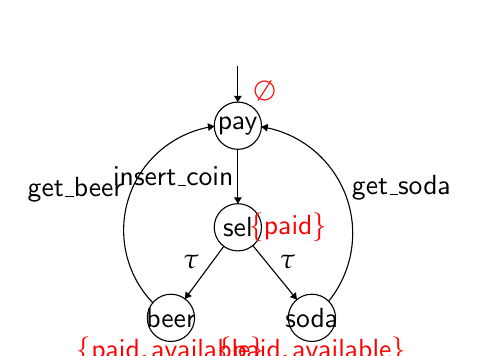
\begin{tikzpicture}[scale=0.10]
			\tikzstyle{every node}+=[inner sep=0pt]
			\draw [black] (38.6,-22.4) circle (3);
			\draw (38.6,-22.4) node {$\mathsf{pay}$};
			\draw [red] (42, -18) node {$\emptyset$};
			\draw [black] (38.6,-35.3) circle (3);
			\draw (38.6,-35.3) node {$\textsf{sel}$};
			\draw [red] (45, -35.3) node {$\{\textsf{paid}\}$};
			\draw [black] (30.1,-46.8) circle (3);
			\draw (30.1,-46.8) node {$\textsf{beer}$};
			\draw [red] (30.1, -51) node {$\{\textsf{paid}, \textsf{available}\}$};
			\draw [black] (48,-46.8) circle (3);
			\draw (48,-46.8) node {$\textsf{soda}$};
			\draw [red] (48, -51) node {$\{\textsf{paid}, \textsf{available}\}$};
			\draw [black] (38.6,-14.8) -- (38.6,-19.4);
			\fill [black] (38.6,-19.4) -- (39.1,-18.6) -- (38.1,-18.6);
			\draw [black] (38.6,-25.4) -- (38.6,-32.3);
			\fill [black] (38.6,-32.3) -- (39.1,-31.5) -- (38.1,-31.5);
			\draw (38.1,-28.85) node [left] {$\textsf{insert\_coin}$};
			\draw [black] (36.82,-37.71) -- (31.88,-44.39);
			\fill [black] (31.88,-44.39) -- (32.76,-44.04) -- (31.96,-43.45);
			\draw (33.77,-39.66) node [left] {$\tau$};
			\draw [black] (40.5,-37.62) -- (46.1,-44.48);
			\fill [black] (46.1,-44.48) -- (45.98,-43.54) -- (45.21,-44.17);
			\draw (43.86,-39.62) node [right] {$\tau$};
			\draw [black] (27.798,-44.886) arc (-136.20523:-262.20742:13.32);
			\fill [black] (35.61,-22.47) -- (34.75,-22.08) -- (34.88,-23.07);
			\draw (24.07,-30.54) node [left] {$\textsf{get\_beer}$};
			\draw [black] (41.591,-22.534) arc (81.15163:-39.01368:13.699);
			\fill [black] (41.59,-22.53) -- (42.3,-23.15) -- (42.46,-22.16);
			\draw (53.02,-30.3) node [right] {$\textsf{get\_soda}$};
			\end{tikzpicture}
		\end{center}
		\caption{Representation of $T_{\text{VM}}$}\label{fig-vmagain}
	\end{marginfigure}
	First, the property that any state with an available drink is preceded by a state where the user has paid can be written formally as\footnote{Note that indices used for $\omega$-words (like $i$ and $j$ for $P_1$) are quantified over all $\omega$ unless stated otherwise.} \[P_1 = \{\sigma \in (2^{\AP})^{\omega} : \forall i, \textsf{available} \in \sigma(i) \implies i>0 \wedge \exists j<i, \textsf{paid} \in \sigma(j)\}.\]
	Intuitively, the system seems to behave according to $P_1$, so one might expect that $T_{\text{VM}}$ \textquotedblleft satisfies\textquotedblright this property in some sense. Definition \ref{defn-satltp} will formalize this intuition.
	
	The property that the number of states where a user has paid is at least as large as the number of states where a drink is available is written: \[P_2 = \left\{\sigma \in(2^{\AP})^{\omega} :\left|\{i \mid \textsf{available} \in \sigma(i)\}\right| \leq \left|\{i \mid \textsf{paid} \in \sigma(i)\}\right| \right\}.\]
	In general, LTPs similar to $P_1$ and $P_2$ are hard to work with because they are not finitary in the sense that, to verify them, one has no choice but to look at an infinite amount of symbols.%TODO: verify this statement.

	We will see that some properties which might look infinitary are easier to automatically verify because they have a finite representation. For instance, the property that there is an infinite number of states is written:\footnote{The notation $\exists^{\infty}$ is a shorthand of  $\forall N, \exists i \geq N$. Its less intuitive dual, \textquotedblleft always true after some point\textquotedblright, is denoted $\forall^{\infty} := \exists N, \forall i\geq N$.}
	\[P_3 = \{ \sigma \in(2^{\AP})^{\omega} \mid \exists^{\infty} i, \textsf{paid} \in \sigma(i)\}.\]
	
	This last LTP illustrates how $\forall^{\infty}$ can be used:
	\[ P_4 = \left\{ \sigma \in(2^{\AP})^{\omega} \mid \left[\forall^{\infty} i, \textsf{paid} \in \sigma(i)\right] \implies \left[\exists^{\infty} i, \textsf{available} \in \sigma(i)\right]\right\}.\]
\end{exmp}
\begin{defn}[Path]
	A (finite or infinite) \textbf{path} in a transition system $T = (S, A, \rightarrow, I, \AP, L)$ is a (finite or infinite) sequence of states $\pi = (s_i)_{i \leq n} \subseteq S$ with $n \leq \omega$ and such that $\forall i, i+1 < n \implies \exists \alpha \in A, s_i \action{\alpha} s_{i+1}$. We say that a path $\pi$ is \textbf{initial} if $s_0 \in I$.
\end{defn}
\begin{defn}[Trace]
	The \textbf{trace} of a path $\pi= (s_i)_{i<n}$ is the sequence $L(\pi) := (L(s_i))_{i<n}$. The \textbf{set of traces} of a transition system $T$, denoted $\Tr(T)$, is 
	\[\Tr(T) = \left\{L(\pi) \mid \pi \text{ is an initial path in $T$}\right\}.\]
	Also, $\Tr^{\omega}(T)$ denotes the set of infinite traces and $\Tr_{\text{fin}}(T)$ the set of finite traces.
\end{defn}
\begin{defn}\label{defn-satltp}
	We say that a transition system $T$ \textbf{satisfies a linear time property} $P$ if $\Tr^{\omega}(T) \subseteq P$. We denote this by write $T\vSim P$.\footnote{We use this notation instead of the more usual $\vDash$ because this definition is not the perfect notion of satisfaction. Informally, this comes from the fact branchings are a feature internal to transition systems but not to LTPs. When we cover modal logics, we will see how to fix this definition.}
\end{defn}
\begin{exmp}
	Let us show that all the properties in Example \ref{exmp-vendingprops} are satisfied by $T_{\text{VM}}$.
	 \begin{enumerate}
	 	\item Clearly, $T_{\text{VM}}\vSim P_1$ because any path in $T$ goes through \textsf{sel} before going through either \textsf{beer} or \textsf{soda}.
	 	\item Since for any $i$ such that $\textsf{available} \in L(\pi_i)$, we also have $\textsf{paid} \in L(\pi)$ it follows trivially that $T_{\text{VM}}\vSim P_2$.
	 	\item The structure of $T_{\text{VM}}$ is very simple and we can observe that for any $\pi$ and any $N\in \N$, $\textsf{paid} \in L(\pi_{N+2})$,\footnote{In words, starting in any state, doing two transition always leads to a state where the user has paid.} thus $T_{\text{VM}} \vSim P_3$.
	 	%any path with more than one state satisfies $\left|\{i \mid \textsf{paid} \notin L(\pi_i)\}\right| \leq \left|\{i \mid \textsf{paid} \in L(\pi_i)\}\right|$. Thus, if $\pi$ is infinite, then so is the number of $i\in \omega$ satisfying 
	 	\item Note that for any infinite path in $T_{\text{VM}}$ goes infinitely many times through \textsf{pay}, thus it is not possible that at some point, any state in the path has \textsf{paid} in its labeling. We conclude that $T_{\text{VM}} \vSim P_4$.
	 \end{enumerate}
\end{exmp}
\begin{prop}\label{prop-sametracesinfty}
	Let $T$ and $T'$ be two transition systems over $\AP$, then 
	\[\Tr^{\omega}(T) \subseteq \Tr^{\omega}(T') \Leftrightarrow \left[\forall P \subseteq (2^{\AP})^{\omega}, (T' \vSim P \implies T \vSim P)\right].\]
\end{prop}
\begin{proof}
	($\Rightarrow$) Follows trivially from the definitions. Indeed, for any $P \subseteq (2^{\AP})^{\omega}$,
	\[T'\vSim P \stackrel{\text{def}}{\Leftrightarrow} \Tr^{\omega}(T') \subseteq P \stackrel{\text{hyp}}{\implies} \Tr^{\omega}(T) \subseteq P \stackrel{\text{def}}{\Leftrightarrow} T \vSim P.\]
	
	($\Leftarrow$) Consider $P = \Tr^{\omega}(T')$. We know that $T' \vSim P$, so, by our hypothesis, $T\vSim P$, that is $\Tr^{\omega}(T) \subseteq \Tr^{\omega}(T')$.\footnote{Although this proof is quite trivial, it illustrates the importance of the fact that infinite traces of a transition system form an LTP.}
\end{proof}
\begin{exmp}
	Let $T'_{\text{VM}}$ be the transition depicted below (we omit the actions as they are irrelevant for this example).
	\begin{center}
		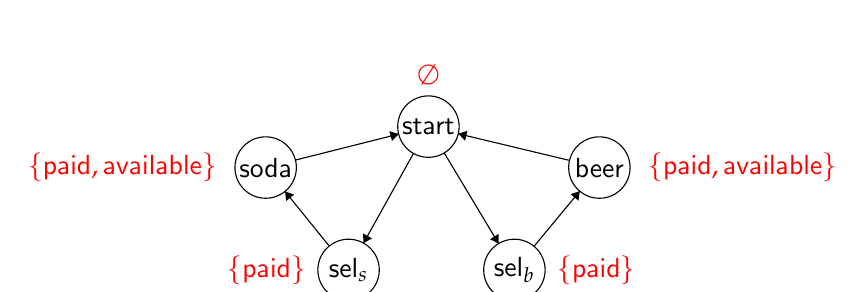
\begin{tikzpicture}[scale=0.13]
		\tikzstyle{every node}+=[inner sep=0pt]
		\draw [black] (39.5,-18.5) circle (3);
		\draw (39.5,-18.5) node {$\textsf{start}$};
		\draw [red] (39.5,-13.5) node {$\emptyset$};
		\draw [black] (31.7,-32.5) circle (3);
		\draw (31.7,-32.5) node {$\textsf{sel}_s$};
		\draw [red] (23.7,-32.5) node {$\{\textsf{paid}\}$};
		\draw [black] (47.9,-32.5) circle (3);
		\draw (47.9,-32.5) node {$\textsf{sel}_b$};
		\draw [red] (55.9,-32.5) node {$\{\textsf{paid}\}$};
		\draw [black] (23.6,-22.5) circle (3);
		\draw (23.6,-22.5) node {$\textsf{soda}$};
		\draw [red] (9.6,-22.5) node {$\{\textsf{paid}, \textsf{available}\}$};
		\draw [black] (56.2,-22.5) circle (3);
		\draw (56.2,-22.5) node {$\textsf{beer}$};
		\draw [red] (70.2,-22.5) node {$\{\textsf{paid}, \textsf{available}\}$};
		\draw [black] (38.04,-21.12) -- (33.16,-29.88);
		\fill [black] (33.16,-29.88) -- (33.99,-29.42) -- (33.11,-28.94);
		\draw [black] (29.81,-30.17) -- (25.49,-24.83);
		\fill [black] (25.49,-24.83) -- (25.6,-25.77) -- (26.38,-25.14);
		\draw [black] (26.51,-21.77) -- (36.59,-19.23);
		\fill [black] (36.59,-19.23) -- (35.69,-18.94) -- (35.94,-19.91);
		\draw [black] (41.04,-21.07) -- (46.36,-29.93);
		\fill [black] (46.36,-29.93) -- (46.37,-28.98) -- (45.52,-29.5);
		\draw [black] (49.82,-30.19) -- (54.28,-24.81);
		\fill [black] (54.28,-24.81) -- (53.39,-25.1) -- (54.16,-25.74);
		\draw [black] (53.28,-21.8) -- (42.42,-19.2);
		\fill [black] (42.42,-19.2) -- (43.08,-19.87) -- (43.31,-18.9);
		\end{tikzpicture}
	\end{center}
	The traces of $T'_{\text{VM}}$ are the same as the traces of $T_{\text{VM}}$. In particular, we have $\Tr^{\omega}(T_{\text{VM}}) = \Tr^{\omega}(T'_{\text{VM}})$, so Proposition \ref{prop-sametracesinfty} says either system satisfies LTPs that the other satisfies.
\end{exmp}
We have already mentioned that some LTPs are harder to verify than others, now we will introduce different families of linear time properties are nicer than most. There are many such families, but we chose three which are simple to define and have both historical and theoretical importance.\footnote{}%TODO: continue this motivation.
\subsection{Invariants and Safety Properties}
\begin{defn}[Invariant]
	A linear time property $P \subseteq (2^{\AP})^{\omega}$ is an \textbf{invariant} if there exists a propositional formula $\phi$ over $\AP$ such that $P = \{\sigma \mid \forall i, \sigma(i) \vDash \phi\}$.\footnote{In words, all the paths of a system satisfying $P$ goes through states that satisfy some property $\phi$.}
\end{defn}
\begin{exmp}
	Recall Example \ref{exmp-handshake} where we ensured mutual exclusion. In the last system $T = A \dmid_{\textsf{rel}, \textsf{req}} (T_1 \tmid T_2)$, the states where both $T_1$ and $T_2$ are in their critical sections are not reachable. Thus, a formula of the form $\phi = \neg(\textsf{c}_1 \wedge \textsf{c}_2)$ is satisfied at any state in a path in $T$. The property of mutual exclusion is thus an invariant.
\end{exmp}
\begin{defn}[Safety Property] 
	A linear time property $P \subseteq (2^{\AP})^{\omega}$ is a \textbf{safety property} if there is a set of finite words $P_{\text{bad}}\subseteq (2^{\AP})^*$ such that\footnote{Intuitively, a safety property is one that always fails in finite time. That is, if $L(\pi) \notin P$, then there exists a finite point in the execution of $\pi$ where we can decide that the trace of $\pi$ is not in $P$.}
	\[P = \left\{\sigma \in (2^{\AP})^{\omega} \mid \forall i \in \N, \sigma(0)\cdots \sigma(i) \notin P_{\text{bad}}\right\}.\]
\end{defn}
\begin{exmp}
	In Example \ref{exmp-vendingprops}, $P_1$ and $P_2$ for $T_{VM}$ are safety properties. For $P_1$, we know that $\sigma$ fails to be in $P$ when \textsf{available} appears before \textsf{paid}, thus we can write\footnote{We use the regular expression notation, where $\texttt{a}^*$ means any finite sequence of $\texttt{a}$, $\texttt{a}\cdot\textsf{b}$ means $\textsf{a}$ followed by $\texttt{b}$ and $\texttt{a} + \texttt{b}$ means an \texttt{a} or a \texttt{b}.}
	\[P_{1,\text{bad}} = \emptyset^* \cdot \bra{\{\textsf{available}\} + \{\textsf{paid}, \textsf{available}\}}.\]
\end{exmp}
Before getting dirty with these family of properties, we show two very simple statements.
\begin{prop}\label{prop-equivdefsafe}
	An LTP $P$ is a safety property if and only if for any $\sigma \in P^{c}$,\footnote{The complement of an LTP $P$ on $\AP$ is $P^c := (2^{\AP})^{\omega} \setminus P$.} there exists $i \in \N$ such that $\sigma(0)\cdots\sigma(i)\cdot (2^{\AP})^{\omega} \cap P = \emptyset$.
\end{prop}
\begin{proof}
	($\Rightarrow$) Since $P$ is a safety property, it is induced by some $P_{\text{bad}}$. If $\sigma \in P^c$, then we infer from the definition that there exists $i\in \N, \sigma(0)\cdots\sigma(i)\in P_{\text{bad}}$. Now, any word in $\sigma(0)\cdots\sigma(i)\cdot (2^{\AP})^{\omega}$ has a finite prefix in $P_{\text{bad}}$, namely $\sigma(0)\cdots\sigma(i)$, so it cannot be in $P$. This direction follows.
	
	($\Leftarrow$) Using the axiom of choice, for any $\sigma \in P^c$, we can choose $i_{\sigma}$ such that $\sigma(0)\cdots\sigma(i_{\sigma})\cdot (2^{\AP})^{\omega} \cap P = \emptyset$. Thus, if we let $P_{\text{bad}} = \{\sigma(0)\cdots\sigma(i_{\sigma}) \mid \sigma \in P^c\}$, we can easily see that no word in $P$ has a finite prefix in $P_{\text{bad}}$\footnote{If for $i \in \N$ and $\sigma \in P$, $\sigma(0)\cdots \sigma(i) \in P_{\text{bad}}$, it contradicts the fact that $\sigma(0)\cdots\sigma(i_{\sigma})\cdot (2^{\AP})^{\omega} \cap P = \emptyset$.} and any word in $P^c$ has a finite prefix in $P_{\text{bad}}$. Therefore, $P$ is the safety property induced by $P_{\text{bad}}$. 
\end{proof}
\begin{prop}
	Any invariant LTP is a safety property.	
\end{prop}
\begin{proof}
	It suffices to let $P_{\text{bad}}$ be the set of finite words with one character not satisfying the invariant. We leave the details as an exercise.
\end{proof}
\begin{defn}
	Given $\sigma \in (2^{\AP})^{\omega}$, a \textbf{finite prefix} of $\sigma$ is $\hat{\sigma} \in (2^{\AP})^*$ such that $\hat{\sigma} = \sigma(0)\dots\sigma(n)$ for $n \in\N$.	We write $\subseteq$ for the relation ``is a finite prefix of``. 
\end{defn}
\begin{defn}
	A state of a transition system is \textbf{terminal} if it has no outward transition.\footnote{Formally, $s \in S$ is terminal if for any $\alpha \in A$ and any $s' \in s$, $s \not\action{\alpha} s'$.}
\end{defn}
\begin{prop}
	Let $T$ be a transition system with no terminal states and $P\subseteq (2^{\AP})^{\omega}$ be a safety property induced by $P_{\text{bad}}$, then \[T \vSim P \Leftrightarrow \Tr_{\text{fin}}(T) \cap P_{\text{bad}} = \emptyset.\]
\end{prop}
\begin{proof}
	($\Leftarrow$) Let $L(\pi)$ be an infinite trace of $T$. Since any of its finite prefix is in $\Tr_{\text{fin}}(T)$, it cannot coincide with a word in $P_{\text{bad}}$. Hence, $L(\pi) \in P$.
	
	($\Rightarrow$) Suppose there exists $\hat{\sigma}\in \Tr_{\text{fin}}(T) \cap P_{\text{bad}}$, we have $\hat{\sigma} = L(\pi)$ for a finite path $\pi$, but since there are no terminal state, we can always add states to $\pi$ and obtain an infinite path $\pi'$ such that $\hat{\sigma} \subseteq L(\pi')$. This means $L(\pi') \notin P$, but it contradicts our assumption that $T \vSim P$.
\end{proof}
\begin{cor}\label{cor-sametracesfinite}\footnote{This result is essentially a characterization similar to Proposition \ref{prop-sametracesinfty} that applies to safety properties. But now, instead of comparing all the traces, we only have to compare the finite traces.}
	Let $T$ and $T'$ be transition systems over $\AP$ with no terminal states, then 
	\[\Tr_{\text{fin}}(T) \subseteq \Tr_{\text{fin}}(T') \Leftrightarrow \left[\forall \text{ safety } P \subseteq (2^{\AP})^{\omega}, (T' \vSim P \implies T \vSim P)\right].\]
\end{cor}
\begin{proof}
	($\Rightarrow$) Follows trivially from the last proposition.
	
	($\Leftarrow$) Consider the safety property induced by $P_{\text{bad}} = (2^{\AP})^* \setminus \Tr_{\text{fin}}(T')$. It is clear that $T'\vSim P$ by the last proposition, thus our assumption gives us $T \vSim P$ or equivalently $\Tr_{\text{fin}}(T) \cap (2^{\AP})^* \setminus \Tr_{\text{fin}}(T')= \emptyset$, it follows that $\Tr_{\text{fin}}(T) \subseteq \Tr_{\text{fin}}(T')$.
\end{proof}
Since, finite traces can be arbitrarily large, it is natural to ask whether comparing finite traces of two systems suffices to compare all the LTPs that they satisfy. This is almost the right intuition, but as usual, infinity breaks our intuition as shown in the following example.
\begin{exmp}
	Let $T$ be the transition system depicted below where the state labeling is written inside the states and states' and actions' names are omitted.
	\begin{center}
		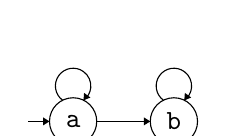
\begin{tikzpicture}[scale=0.1]
		\tikzstyle{every node}+=[inner sep=0pt]
		\draw [black] (32.1,-21.3) circle (3);
		\draw (32.1,-21.3) node {$\texttt{a}$};
		\draw [black] (44.9,-21.3) circle (3);
		\draw (44.9,-21.3) node {$\texttt{b}$};
		\draw [black] (35.1,-21.3) -- (41.9,-21.3);
		\fill [black] (41.9,-21.3) -- (41.1,-20.8) -- (41.1,-21.8);
		\draw [black] (26.4,-21.3) -- (29.1,-21.3);
		\fill [black] (29.1,-21.3) -- (28.3,-20.8) -- (28.3,-21.8);
		\draw [black] (43.577,-18.62) arc (234:-54:2.25);
		\fill [black] (46.22,-18.62) -- (47.1,-18.27) -- (46.29,-17.68);
		\draw [black] (30.777,-18.62) arc (234:-54:2.25);
		\fill [black] (33.42,-18.62) -- (34.3,-18.27) -- (33.49,-17.68);
		\end{tikzpicture}
	\end{center}
	We have $\Tr_{\text{fin}}(T) = \texttt{a}^*\texttt{b}^*$ and $\Tr^{\omega}(T) = \texttt{a}^*\texttt{b}^{\omega} + \texttt{a}^{\omega}$. Now consider for any $i \in \N$, the system $T_i$ as depicted below (with the same conventions as for $T$).
	\begin{center}
		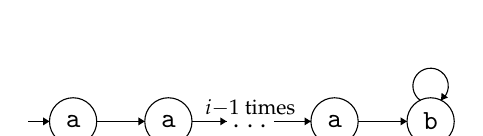
\begin{tikzpicture}[scale=0.1]
		\tikzstyle{every node}+=[inner sep=0pt]
		\draw [black] (22.8,-21.3) circle (3);
		\draw (22.8,-21.3) node {$\texttt{a}$};
		\draw [black] (68.2,-21.3) circle (3);
		\draw (68.2,-21.3) node {$\texttt{b}$};
		\draw [black] (34.9,-21.3) circle (3);
		\draw (34.9,-21.3) node {$\texttt{a}$};
		\draw [black] (56,-21.3) circle (3);
		\draw (56,-21.3) node {$\texttt{a}$};
		\draw (45.3,-20.5) node {$\stackrel{i-1\text{ times}}{\cdots}$};
		\draw [black] (17.1,-21.3) -- (19.8,-21.3);
		\fill [black] (19.8,-21.3) -- (19,-20.8) -- (19,-21.8);
		\draw [black] (66.877,-18.62) arc (234:-54:2.25);
		\fill [black] (69.52,-18.62) -- (70.4,-18.27) -- (69.59,-17.68);
		\draw [black] (25.8,-21.3) -- (31.9,-21.3);
		\fill [black] (31.9,-21.3) -- (31.1,-20.8) -- (31.1,-21.8);
		\draw [black] (37.9,-21.3) -- (42.3,-21.3);
		\fill [black] (42.3,-21.3) -- (41.5,-20.8) -- (41.5,-21.8);
		\draw [black] (48.3,-21.3) -- (53,-21.3);
		\fill [black] (53,-21.3) -- (52.2,-20.8) -- (52.2,-21.8);
		\draw [black] (59,-21.3) -- (65.2,-21.3);
		\fill [black] (65.2,-21.3) -- (64.4,-20.8) -- (64.4,-21.8);
		\end{tikzpicture}
	\end{center}
	The finite traces of $T_i$ will be words recognized by $\texttt{a}+ \cdots + \texttt{a}^i \cup \texttt{a}^i\texttt{b}^*$ and its infinite traces will be recognized by $\texttt{a}^i\texttt{b}^{\omega}$.
	
	Now, let $T'$ be the union\footnote{Informally, it is like putting all systems next to each other with no interaction between them. All initial states of the $T_i$'s are still initial states, so the paths in $T'$ are just the union of the paths in the $T_i$'s.} for $i \in \N$ of the $T_i$'s, then we have $\Tr_{\text{fin}}(T') = \texttt{a}^*\texttt{b}^* = \Tr_{\text{fin}}(T)$, but $\Tr^{\omega}(T') = \texttt{a}^*\texttt{b}^{\omega} \neq \Tr^{\omega}(T) $.
\end{exmp}
The following definition introduces a sufficient condition to get rid of such counterexamples. As expected, it is a finiteness property.
\begin{defn}[Finitely Branching]
	A transition system $T$ is said to be \textbf{finitely branching} if $I$ is finite and for any $s \in S$, $\{s'\in S \mid \exists \alpha \in A, s \action{\alpha} s'\}$ is finite.\footnote{In later parts of the course, we will study logics that will care about what actions are used. In these cases, finitely branching will require that there is a finite number of distinct actions that can be done at $s$.}
\end{defn}
\begin{prop}\label{prop-finbranchtraces}
	Two finitely branching $T$ and $T'$ with no terminal states and on $\AP$ satisfy \[\Tr^{\omega}(T) \subseteq \Tr^{\omega}(T') \Leftrightarrow \Tr_{\text{fin}}(T) \subseteq \Tr_{\text{fin}}(T').\]
\end{prop}
\begin{proof}
	($\Rightarrow$) Since the systems have no terminal states, any finite trace in $T$ corresponds to a path $\pi$ in $T$ that can be extended to an infinite path $\pi'$ so that $L(\pi')$ is in $\Tr^{\omega}(T)$ and thus in $\Tr^{\omega}(T')$. Now, $L(\pi')$ must correspond to a path $\pi''$ in $T'$ and truncating it to the size of $\pi$ shows that $L(\pi) = L(\pi''|_{i\leq |\pi|})$ is also in $\Tr_{\text{fin}}(T')$.
	
	($\Leftarrow$)\footnote{In class, this direction was proved as a corollary of the more general K\"onig's lemma which states that any finitely branching infinite tree has an infinite path. I chose to integrate the proof of the lemma into the proof of the proposition to avoid introducing more definitions than needed.} Let $\sigma \in \Tr^{\omega}(T)$, for any $n\in \N$, $\sigma_n := \sigma(0)\cdots \sigma(n) \subseteq \sigma$ is in $\Tr_{\text{fin}}(T) \subseteq \Tr_{\text{fin}}(T')$, so in particular, it is the finite trace of an initial path, say $\pi_n$, in $T'$.
	
	To construct an initial path $\pi$ in $T'$ that satisfies $L(\pi) = \sigma$, we will build $(s_i)_{i\in\N}$ by induction on $i$ with $s_0 \in I$ and the following invariant: There are infinitely many $\pi_n$'s such that $\forall k\leq i, \pi_n(k) = s_k$.
	
	First, since $I'$ is finite and all paths $\pi_n$ satisfy $\pi_n(0)\in I'$, there is at least one $s_0 \in I'$ such that there are infinitely many $\pi_n$ with $\pi_n(0) = s_0$.
	
	Second, suppose $s$ is defined up to $i-1$ and there are infinitely many $\pi_n$'s satisfying $P_{i-1}:=\forall k\leq i-1, \pi_n(k) = s_k$. Then, since there are finitely many $s\in S'$ such that $s_{i-1}\action{\alpha} s$ for some $\alpha \in A'$, we can pick one such $s_i$ such that there are still infinitely many of the $\pi_n$ satisfying $P_{i-1}$ that satisfy $P_i := \forall k\leq i, \pi_n(k) = s_k$.
	
	By the induction principle, this defines a path $\pi = (s_i)_{i\in \N}$ that 
	\begin{enumerate}
		\item is initial because $s_0 \in I'$,
		\item is in $T'$ because every finite subpath is in $T'$, and 
		\item satisfies $L(\pi) = \sigma$ because $L(\pi_n) = \sigma_n$ for all $\pi_n$.
	\end{enumerate}
	We conclude that $\sigma \in \Tr^{\omega}(T')$.
\end{proof}
\begin{cor}
	Two transition systems on $\AP$ with no terminal states satisfy the same LTPs if and only if they satisfy the same safety properties.
\end{cor}
\begin{proof}
	The proof follows from these equivalences that use the previous results:
	\begin{align*}\left[\forall P \in (2^{\AP})^{\omega}, T \vSim P \Leftrightarrow T' \vSim P\right] &\Leftrightarrow \Tr^{\omega}(T) = \Tr^{\omega}(T') \\&\Leftrightarrow \Tr_{\text{fin}}(T) = \Tr_{\text{fin}}(T')\\
	&\Leftrightarrow \left[\forall \text{ safety }P \in (2^{\AP})^{\omega}, T \vSim P \Leftrightarrow T' \vSim P\right] \end{align*}
\end{proof}

%The proof relies on König's lemma, but before that we need a bit more definitions.
%\begin{defn}
%	Fix a set $A$.
%	\begin{enumerate}
%		\item A \textbf{tree} on $A$ is a set $T \subseteq A^*$ that is closed under prefix.\footnote{For any $u \in T$ for any $w\subseteq u$, $w \in T$. They are called trees because it is natural to represent them as trees, taking the root to be $\varepsilon$ and each word has its immediate prefix as its parent.}
%		\item $T$ is \textbf{finitely branching} if for any $u \in T$, the set of children of $u$ (i.e.: $\{ua \mid a \in A\}$) is finite.\footnote{Note that any tree on a finite alphabet is finitely branching.}
%		\item A \textbf{path} is a $\omega$-word $(a_i)_{i \in \N} \in A^{\omega}$ such that $\forall i \in \N, a_0\cdots a_i \in T$.
%	\end{enumerate}
%\end{defn}
%\begin{lem}[König]
%	Any finitely branching infinite tree $T$, then it has a path (infinite).
%\end{lem}
%\begin{proof}
%	Given a tree $T \subseteq A^*$ and $u \in A^*$, we denote $T\upharpoonright u = \{v \in T \mid u \subseteq v \text{ or } v \subseteq u\}$.
%	
%	We define by induction on $n$, a sequence $a_0, \dots, a_n$ of letters in $A$ satisfying $a^n = a_0\cdots a_n \in T$ and $T\upharpoonright a^n$ is infinite.
%	
%	The base case is trivial because $T$ is infinite.
%	
%	Suppose $a_0, \dots, a_{n-1}$ are defined. Then, we can write $T \upharpoonright a^{n-1} = \cup_{a \in A} \upharpoonright a^{n-1}a$. But since the tree is finitely branching, only finitely many of the elements of this union are not empty. Thus, because $T\upharpoonright a^{n-1}$ is infinite and by the pigeonhole principle, for at least one $a$, $T \upharpoonright a^{n-1}a$ is infinite.
%	
%	The sequence defined is a path by invariant 1).
%\end{proof}
We will end this section with a bit more terminology and practice with results on invariants and safety properties.
\begin{defn}[Closure]\label{defn-prefixesandclosure}
	Let $P$ be an LTP, we denote the set of finite prefixes of $P$ by \[\pref(P) = \{\hat{\sigma} \in (2^{\AP})^* \mid \exists \sigma \in P, \hat{\sigma} \subseteq \sigma \}.\] %TODO: explain extension to single LTPs.
	The \textbf{closure} of $P$ is the set of LTPs that have all their finite prefixes in $P$, that is,
	\[ \cl(P) = \{\sigma \in (2^{\AP})^{\omega} \mid \pref(\sigma) \subseteq \pref(P)\}.\]
\end{defn}
\begin{prop}\label{prop-safeclos}
	An LTP $P$ is a safety property if and only if $\cl(P) = P$.
\end{prop}
\begin{proof}
	($\Rightarrow$) Note that $P \subseteq \cl(P)$ is trivially true for any $P$.\footnote{One way to see this is: \[\pref(P) = \bigcup_{\sigma \in P} \pref(\sigma).\]} Now, suppose that $\sigma \in \cl(P)$, for any finite prefix  $\hat{\sigma} \subseteq \sigma$, $\hat{\sigma} \in \pref(P)$, so there exists $\sigma'$ with $\hat{\sigma} \subseteq \sigma'$. In other words, $\hat{\sigma}\cdot (2^{\AP})^{\omega}\cap P \neq \emptyset$ and we conclude that $\sigma \in P$ by the contrapositive of Proposition \ref{prop-equivdefsafe}.
	
	($\Leftarrow$) Let $\sigma \in P^c$, in particular $\sigma \notin \cl(P)$, so there is a finite prefix $\hat{\sigma}\subseteq \sigma$ that is not the prefix of any word in $P$. In mathematical terms, this means $\hat{\sigma}\cdot (2^{\AP})^{\omega}\cap P = \emptyset$. Since $\sigma$ was arbitrary, $P$ is a safety property by Proposition \ref{prop-equivdefsafe}.
\end{proof}
\begin{prop}
	Let $P$ and $Q$ be safety properties, then $P \cup Q$ and $P \cap Q$ are also safety properties.
\end{prop}
\begin{proof}%TODO: write from which TD this is.
	For the union, since a word is in $P \cup Q$ if it has no finite prefix in one of $P_{\text{bad}}$ and $Q_{\text{bad}}$, it follows that $P\cup Q$ is the safety property induced by $(P\cup Q)_{\text{bad}} := P_{\text{bad}} \cap Q_{\text{bad}}$.
	
	For the intersection, it follows from Proposition \ref{prop-safeclos} and 
	\[\cl(P) \cap \cl(Q) = \bigcup_{\sigma \in P} \pref(\sigma) \bigcap \bigcup_{\sigma \in Q} \pref(\sigma) = \bigcup_{\sigma \in P\cap Q} \pref(\sigma) = \cl(P\cap Q).\]
\end{proof}


\subsection{Liveness Properties}
%TODO: Our third family, liveness properties are : something good will always happen but a bit less finitary.
\begin{defn}[Liveness]
	A LTP $P \subseteq (2^{\AP})^{\omega}$ is a \textbf{liveness} property if for any $\hat{\sigma} \in (2^{\AP})^*$, there exists $\sigma \in (2^{\AP})^{\omega}$ such that $\hat{\sigma} \subseteq \sigma$ and $\sigma \in P$.
\end{defn}
\begin{exmp}
	The system $T_{\text{VM}}$ from Example \ref{exmp-vending} satisfies the property \[P=\{\sigma \mid \exists^{\infty} i, \textsl{available}\in \sigma(i) \implies \exists^{\infty} i, \textsl{paid} \in \sigma(i)\},\]
	because both sides of the implication are true for any $\sigma \in \Tr^{\omega}(T_{\text{VM}})$.\footnote{}%TODO:Note that $P$ is really infinitary, in the sense that it is not something good that will happen in the finite run.}
	$P$ is a liveness property because any finite word can be completed with $(\{\textsf{available}\}\{\textsf{paid}\})^*$.
\end{exmp}
\begin{prop}\label{prop-livepref}
	An LTP $P$ is a liveness property if and only if $\pref(P) = (2^{\AP})^*$.
\end{prop}
\begin{proof}
	($\Rightarrow$) Suppose there exists $\sigma \in (2^{\AP})^*\setminus \pref(P)$, then $\sigma$ could not be extended into a word of $\sigma$, contradicting the liveness of $P$.
	
	($\Leftarrow$) Any finite word is in $\pref(P)$, thus it can be extended in a word of $P$. We conclude that $P$ is a liveness property.
\end{proof}
\begin{cor}
	Let $P$ and $Q$ be liveness properties on $\AP$, then $P \cup Q$ is also a liveness property.\footnote{It follows from Proposition \ref{prop-livepref} because $\pref(P\cup Q) = \pref(P) \cup \pref(Q)$.}
\end{cor}
\begin{exmp}
	Unlike for safety properties, the intersection of two liveness properties is not always a liveness property. Consider the following properties:\footnote{$P$ and $Q$ respectively contain all $\omega$-words that are eventually all \texttt{1}s and all \texttt{0}s.}
	\begin{align*}
		P &= \{\sigma \in \{\texttt{0},\texttt{1}\}^\omega \mid \forall^{\infty}i, \sigma(i) = \texttt{1}\}\\
		Q &= \{\sigma \in \{\texttt{0},\texttt{1}\}^\omega \mid \forall^{\infty}i, \sigma(i) = \texttt{0}\}.\\
	\end{align*}
	They are both clearly liveness as any finite word can be completed with either $\texttt{1}^{\omega}$ or $\texttt{0}^{\omega}$ and belong to $P$ or $Q$ respectively. However, their intersection is clearly empty and $\emptyset$ is not a liveness property.
\end{exmp}
%TODO: Maybe new subsectin for this.
%TODO:Safety properties are often stoked together with liveness properties. (Idea is that in order to ensure safety, just do nothing.)

\begin{prop}\label{prop-onlyliveandsafe}
	The property $\top := (2^{\AP})^{\omega}$ is the only LTP that is a liveness and safety property.
\end{prop}
\begin{proof}
	Since any finite word can be completed into an $\omega$-word, $\top$ is liveness. It is also safety induced by $P_{\text{bad}} = \emptyset$.
	
	Let $P$ be a safety property induced by $P_{\text{bad}}$, then any $x \in P_{\text{bad}}$ cannot be extended into a infinite path in $P$ by definition. Therefore, if $P$ is safety and liveness, $P_{\text{bad}}$ must be empty and $P = \top$.
\end{proof}
%TODO: motivation for theorem
\begin{thm}[Decomposition]\label{thm-decompltp}
	Any LTP $P$ can be decomposed in a liveness property and safety property. $P = P_{\text{safe}} \cap P_{\text{live}}$.
\end{thm}

In order to prove this theorem, we will introduce two very different approaches that lead to very elegant proofs. Thus, the two next sections will feel ad hoc at first, but they are very much used in current research in semantics, so they are worth covering.

\section{Topological Spaces}
\subsection{Preliminaries}
Not much theory is needed, but we present it here for completeness.
\begin{defn}\label{defn-topspace}
	A \textbf{topological space} is a pair $(X, \Omega X)$, where $X$ is a set and $\Omega X\subseteq 2^X$ is a set that is closed under arbitrary unions and finite intersections\footnote{For any family of open sets $\{U_i\}_{i \in I}$,\[\bigcup_{i \in I} U_i \in \Omega X,\] and if $I$ is finite,\[\bigcup_{i \in I} U_i \in \Omega X.\]} whose elements are called \textbf{open sets} of $X$.
	
	Complements of open sets (denoted $U^c$) are called \textbf{closed sets}. Observe that both the empty set and the whole space are open and closed (sometimes referred to as \textbf{clopen}) because 
	\[\emptyset = \bigcup_{U \in \emptyset} U \text{ and } X = \bigcap_{U \in \emptyset} U.\]
\end{defn}
%TODO: make this clear
%For our purpose, $\Omega$ should be seen as the sets that are semi-observable, where semi is very similar in meaning to the semi-computable terminology. The idea is that we can realize we are in an open set in finite time, but we might not find whether we are not in an open set in finite time. (note that we did not use the closed because of the following lemma) The definition gives this because we can semi-decide an infinite conjunction and a finite conjunction.

All the following terminology and results are basic tools use in topology that will end up helping us prove the decomposition theorem. Fix a topological space $(X,\Omega X)$.
\begin{lem}
	Let $(C_i)_{i \in I}$ be a family of closed sets of $X$, then $\cap_{i \in I} C_i$ is closed and if $I$ is finite, $\cup_{i \in I} C_i$ is also closed.\footnote{Observe that this are statements dual to the axioms of Definition \ref{defn-topspace}. In fact, it is sometimes more convenient to define a topological space by giving its closed sets, and it is equivalent.}
\end{lem}
\begin{proof}
	Both statements follow trivially from DeMorgan's laws and the fact that the complement of a closed set is open and vice-versa. For the first one, DeMorgan's laws yield
	\[\bigcap_{i \in I} C_i =  \bra{\bigcup_{i \in I} C_i^c}^c,\]
	and the LHS is the complement of a union of opens, so it is closed. For the second one, DeMorgan's laws yield
	\[\bigcup_{i \in I} C_i =  \bra{\bigcap_{i \in I} C_i^c}^c,\]
	and the LHS is the complement of a finite intersection of opens, so it is closed.
\end{proof}
\begin{lem}\label{lem-openchar}
	A subset $A \subseteq X$ is open if and only if for any $x \in A$, there exists an open $U \subseteq A$ such that $x \in A$.
\end{lem}
\begin{proof}
	($\Rightarrow$) For any $x \in A$, set $U = A$.
	
	($\Leftarrow$) For each $x \in X$, pick an open $U_x \subseteq A$ such that $x \in A$, then we claim $A = \cup_{x \in A} U_x$ which is open\footnote{Arbitrary unions of opens are open.}. The $\subseteq$ inclusion follows because each $x \in A$ has a set $U_x$ in the union that contains $x$. The $\supseteq$ inclusion follows because each term of the union is a subset of $A$ by assumption.
\end{proof}
\begin{lem}\label{lem-closedchar}
	A subset $A\subseteq X$ is closed if and only if for any $x \notin A$, there exists an open $U$ such that, $x \in U$ and $U\cap A = \emptyset$.\footnote{This result is simply a restatement of the last one by setting $A = A^c$.}
\end{lem}
\begin{defn}
	Given $A \subseteq X$, the \textbf{closure} of $A$ is \[\overline{A} := \bigcap \{C \text{ closed}\mid C \supseteq A \}.\]
	It is very easy to show that $\overline{A}$ is the smallest closed set containing $A$.\footnote{$\overline{A}$ is closed because it is an intersection of closed sets and any closed sets containing $A$ also contains $\overline{A}$ by definition.} Then, it follows that $A$ is closed if and only if $\overline{A} = A$.
\end{defn}
Here are more easy results on the closure of a subset.
\begin{lem}\label{lem-closure}
	Given $A,B \subseteq X$ then the following statements hold:
	\marginnote{
		\begin{proof}[Proof of Lemma \ref{lem-closure}]
			\begin{enumerate}
				\item By definition, $\overline{B}$ contains $B$, thus $A$, but $\overline{B}$ is closed, so it must contain $\overline{A}$.
				\item By definition.
				\item $\overline{A}$ is closed, so its closure is itself.
				\item 3 applied to $\emptyset$.
				\item $\subseteq$ follows because the LHS is the smallest closed set containing $A \cup B$ and the RHS is closed and contains $A\cup B$.\\ $\supseteq$ follows because the LHS is a closed set containing $A$ and $B$, it contains $\overline{A}$ and $\overline{B}$.%TODO: follows ?
			\end{enumerate}
		\end{proof}}
	\begin{enumerate}
		\item $A \subseteq B \implies \overline{A} \subseteq \overline{B}$.
		\item $A \subseteq \overline{A}$
		\item $\overline{\overline{A}} = \overline{A}$.
		\item $\overline{\emptyset} = \emptyset$
		\item $\overline{A \cup B} = \overline{A} \cup \overline{B}$.
	\end{enumerate}
	%TODO: put this in footnote : Closure operators satisfy 1-3 and Kuratowski operators satisfy 1-5 (they generate the closed sets of a topology). Sometimes useful in lattice theory or boolean algebras.
\end{lem}

\begin{defn}
	A subset $A\subseteq X$ is said to be \textbf{dense} (in $X$) if any non-empty open set intersects $A$ non-trivially, that is, $\forall U \neq \emptyset \in \Omega X, A \cap U \neq \emptyset$.
\end{defn}
\begin{thm}[Decomposition]\label{thm-decomptop}
	Let $A\subseteq X$, then $A = \overline{A} \cap (A \cup \overline{A}^c)$, where $\overline{A}$ is closed and $A \cup \overline{A}^c$ is dense.\footnote{This results says that any set can be decomposed into a closed and a dense set. Note the similarity with Theorem \ref{thm-decompltp}, we will see that the latter is a corollary of this basic result in topology.}
\end{thm}
\begin{proof}
	The equality is trivial and $\overline{A}$ is closed by definition. It is left to show that $A \cup \overline{A}^c$ is dense. 
	
	Let $U \neq \emptyset$ be an open set. If $U$ intersects $A$, we are done. Otherwise, we have the following equivalences:\[U \cap A = \emptyset\Leftrightarrow A \subseteq U^c \Leftrightarrow \overline{A} \subseteq U^c \Leftrightarrow U \subseteq \overline{A}^c,\]
	where the second $\implies$ holds because $U^c$ is closed. We conclude $U \cap (A \cup \overline{A}^c) \neq \emptyset$.
\end{proof}
\begin{lem}
	A subset $A \subseteq X$ is dense if and only if $\overline{A} = X$.
\end{lem}
\begin{proof}
	($\Rightarrow$) Since $\overline{A}^c$ is open but it intersects trivially a dense set $A$, it must be empty, thus $\overline{A}$ is the whole space.
	
	($\Leftarrow$) Let $U$ be an open set such that $U \cap A = \emptyset$, then $A$ is contained in the closed set $U^c$, but this implies $\overline{A} \subseteq U^c$,\footnote{Recall that the closure of $A$ is the smallest closed set containing $A$.} thus $U$ is empty.
\end{proof}
\begin{defn}
	Let $A \subseteq X$, the \textbf{interior} of $A$ is \[\interior{A} := \bigcup \{U \in \Omega X \mid  U\subseteq A\}.\]
	It is obvious that $\interior{A}$ is the largest open subset of $A$ and thus that $A$ is open if and only if $A = \interior{A}$.\footnote{It also follows that $A \subseteq B \implies \interior{A} \subseteq \interior{B}$ and that $\interior{\interior{A}} = \interior{A}$.} 
\end{defn}

Finally, we end this these preliminaries with a result on how to specify a topology.
\begin{defn}[Base]%TODO: look at other sources.
	Let $X$ be a set, a \textbf{base} $B$ is a set $B\subseteq 2^X$ such that $X = \cup_{U \in B} U$ and any finite intersection of sets in $B$ can be written as a union of sets in $B$. 
\end{defn}
\begin{lem}
	Let $X$ and $B \subseteq 2^X$, then $\Omega X$ be the set of all unions of sets in $B$, $(X,\Omega X)$ is a topology. We say that $\Omega X$ is the topology \textbf{generated} by $B$.
\end{lem}
\begin{proof}
	We know that unions of opens are open and finite intersections of sets in $B$ are open. It remains to show that finite intersections of unions of sets in $B$ are also open. Let $U = \cup_{i \in I} U_i$ and $V = \cup_{j \in J} V_j$ with $U_i \in B$ and $V_j \in B$, then by distributivity, we obtain
	\[U\cap V = \cup_{i \in I} U_i \bigcap \cup_{j \in J} V_j = \bigcup_{i\in I, j \in J} U_i \cap V_j,\]
	so $U \cap V$ is open (being a union of opens). The lemma then follows by induction.
\end{proof}
In practice, instead of generating a topology from a base $B$, we start with any family $B_0 \subseteq 2^X$ and consider its closure under finite intersections $B$, so that it satisfies the axioms of a base. Such a $B_0$ is often called a \textbf{subbase} for the topology generated by $B$. 

Although we could indefinitely extend this digression in topology, we will stop now that we have the essentials and see how this relates to our investigation on linear time properties.

\subsection{$\omega$-words}
\begin{defn}[Extensions]
	Given a non-empty set $A$ and a finite word $u \in A^*$, we denote the extensions of $u$ by\footnote{We write $\ext(u)$ when the alphabet is clear from context. Note that $A^{\omega} = \ext_A(\varepsilon)$.}
	\[\ext_A(u) := u\cdot A^{\omega} = \{ \sigma \in A^{\omega} \mid u\subseteq \sigma\}.\]
	We generalize this notation to sets of finite words $W \subseteq A^*$ in the natural way: \[\ext(W) = \{ \ext(u) \mid u \in W\}.\]
\end{defn}
\begin{prop}
	Let $A$ be a non-empty set, the set\footnote{Notice that this topology is generated by the subbase with containing $\ext(u)$ for any $u \in A^*$ as $\ext(W)$ is the union of such sets when $W \subseteq A^*$.} \[ \Omega A = \left\{ \ext(W) \mid W \subseteq A^* \right\} \]
	is a topology for $A^{\omega}$.
\end{prop}
\begin{proof}
	Let $\{U_i\}_{i \in I}$ be a family of opens, for any $i \in I$, there exists $W_i \subseteq A^*$ such that $U_i = \ext(W_i)$. Then,\footnote{The last equality holds because an $\omega$-word extends a word in one of the $W_i$'s if and only if it extends the same word in the union of the $W_i$'s.}
	\[\cup_{i \in I} U_i = \cup_{i \in I}\ext(W_i) = \ext\bra{\cup_{i \in I} W_i},\]
	so we conclude that $\Omega A$ is closed under unions.
	
	Furthermore, we observe that\footnote{Indeed, if $u\subseteq v$, then any $\omega$-word that extends $v$ also extends $u$, so $\ext(v) \subseteq \ext(u)$. The argument is symmetric for $v\subseteq u$ and if $v$ and $u$ are not comparable, then they do not agree at some index and no $\omega$-word can have two distinct symbols at this index.} \[\ext(u) \cap \ext(v) = \begin{cases}\ext(u) & v \subseteq u\\\ext(v) &u\subseteq v\\ \emptyset &\text{o/w}\end{cases}.\]
	Thus, let $W_1, W_2 \subseteq A^*$, we have 
	\begin{align*}
	\ext(W_1) \cap \ext(W_2) &= \cup_{u \in W_1} \ext(u) \bigcap \cup_{v \in W_2} \ext(v)\\ &= \bigcup_{u \in W_1, v \in W_2} \ext(u) \cap \ext(v)\\ 
	&= \bigcup \{\ext(u) \mid u \in W_1,\exists v\in W_2, v \subseteq U\} \\ &\quad \quad \cup \bigcup \{\ext(v) \mid v \in W_2, \exists u \in W_1, u \subseteq v\}
	\\&= \ext(W_1 \Cap W_2),
	\end{align*}
	where $W_1 \Cap W_2$ is the set of words in one of the $W_i$'s that have a prefix in the other, that is, \[W_1 \Cap W_2 = \{u \in A^* \mid \exists i\neq j, \exists v \in W_j, u\in W_i, v\subseteq u\}.\]
	We conclude that $\Omega A$ is also closed under finite intersection, so it is a topology for $A^{\omega}$.
\end{proof}
From now on, unless otherwise said, we assume that the topology on $A^{\omega}$ is generated by $\Omega A$ given above.
\begin{rem}\label{rem-openchar}
	A set $P \subseteq A^{\omega}$ is open if and only if there exists $W \in A^*$ such that $P = \ext(W) = \cup_{u \in W} \ext(u)$. In particular, if $\sigma \in P$, then there exists $\hat{\sigma} \subseteq \sigma$ such that $\ext(\hat{\sigma}) \subseteq P$.\footnote{In other words, we will know that $\sigma \in P$ after observing it for a finite amount of time because we know all extensions of $\hat{\sigma}$ are in $P$.}
	
	%TODO: Do the same for liveness. On the other hand, if $P$ is closed, then $\sigma \in P$ if and only if for all finite prefixes $\hat{\sigma} \subseteq \sigma$, $\ext(\hat{\sigma}) \cap P \neq \emptyset$.
\end{rem}
If we stare at this remark long enough, we can recover the intuition behind safety LTPs and in particular, the equivalent definitions seen in Proposition \ref{prop-equivdefsafe}. Indeed, the tools we have developed lead to a nice characterization of safety and liveness properties.
\begin{lem}
	An LTP $P \subseteq (2^{\AP})^{\omega}$ is a safety property if and only if it is closed.\footnote{In the usual topology on $\omega$-words.}
\end{lem}
\begin{proof}
	($\Leftarrow$) We have just said that if $\sigma$ is in an open (in this case $P^c$), then there exists $\hat{\sigma} \subseteq \sigma$ such that $\ext(\hat{\sigma}) \subseteq P^c$, i.e. $\ext(\hat{\sigma}) \cap P = \emptyset$ as required for safety properties.
	
	($\Rightarrow$) Let $P$ be induced by $P_{\text{bad}}$, any extension $\sigma$ of a word in $P_{\text{bad}}$ is not in $P$. In other words $P^c = \ext(P_{\text{bad}})$ which is open, thus $P$ is closed.
\end{proof}
\begin{lem}
	An LTP $P \subseteq (2^{\AP})^{\omega}$ is a liveness property if and only if it is dense.
\end{lem}
\begin{proof}
	($\Rightarrow$) Let $U =\emptyset$ be open, then $U = \cup_{u \in W} \ext(u)$, where $W$ cannot be empty. Hence, since for any $u \in W$, $\ext(u) \cap P \neq \emptyset$\footnote{Because any finite word can be extended (by liveness).}, $P\cap U \neq \emptyset$ and this direction follows.
	
	($\Leftarrow$) Let $P$ be dense, then for any $u$, $\ext(u)$ is open, so $P\cap \ext(u) \neq \emptyset$ which means we can extend $u$ to be in $P$. This direction follows.
\end{proof}
\begin{cor}
	Theorem \ref{thm-decompltp}.\footnote{Indeed, any set can be written as the intersection of a closed set and a dense set by Theorem \ref{thm-decomptop}, which are respectively safety and liveness properties.}
\end{cor}
As we mentioned before, we have not gone through all this theory only to prove this theorem, these concepts will come back in this class as well as in a more advanced study of semantics. However, before going back to the main point of this class, we keep our promise of giving two proofs of the decomposition theorem. Therefore, in the next section, we will revisit this characterization through the point of view of lattice theory.

\section{Posets and Complete Lattices}
\subsection{Preliminaries}
%As it true as it was for the last section, we will arrive at the decomposition theorem, the real motivation for seeing this approach is to get algebraic tools that will be useful for later.
\begin{defn}
	A \textbf{poset} (short for partially ordered set) is a pair $(A, \leq)$ where $A$ is a set and $\leq\ \subseteq A \times A$ is a reflexive, transitive and antisymmetric binary relation.
\end{defn}
A prototypical example of a poset which is paradigmatic in this course is the powerset with binary relation being inclusion :$(2^X, \subseteq)$. The restriction of this poset to the opens $\Omega X$ of a topological space also yields an important poset: $(\Omega X, \subseteq)$.
\begin{defn}
	A function $f:(A, \leq_A) \rightarrow (B,\leq_B)$ between posets is \textbf{monotone} (or \textbf{order-preserving}) if for any $a, a' \in A$, $a \leq a' \implies f(a) \leq f(a')$.
\end{defn}
\begin{exmp}
	The closure in a topological space $X$ is a monotone function from $(2^X, \subseteq)$ to itself because $A\subseteq B$ implies $\overline{A} \subseteq \overline{B}$.
\end{exmp}
\begin{defn}
	The \textbf{dual} of a poset $(A, \leq)$ is denoted $\op{(A, \leq)} := (A, \geq)$, where for any $a,a' \in A$, $a' \geq a \Leftrightarrow a\leq a'$.\footnote{This definition lets us avoid many symmetric arguments.}%TODO: better.
\end{defn}
\begin{defn}
	Let $(A, \leq)$ be a poset and $S \subseteq A$, then $a \in A$ is an \textbf{upper bound} of $S$ if $\forall s \in S, s\leq a$. Moreover, $a \in A$ is the \textbf{supremum} of $S$, denoted $\vee S$, if it is the least upper bound, that is, $a$ is an upper bound of $S$ and for any upper bound $a'$ of $S$, $a\leq a'$.
	
	Dually, $a \in A$ is \textbf{a lower bound} (resp. \textbf{infimum}) of $S$ if and only if it is an upper bound (resp. supremum) of $S$ in $\op{(A, \leq)}$.
\end{defn}
\begin{prop}
	Infimums and supremums are unique when they exist.\footnote{By antisymmetry.}
\end{prop}

\begin{defn}
	A \textbf{complete lattice} is the data $(L, \wedge, \vee, \leq)$ where $(L, \leq)$ is a poset, and $\wedge, \vee : (2^L, \subseteq) \rightarrow (L, \leq)$ are respectively infimum (or \textbf{meet}) and the supremum (or \textbf{join}) as defined above.\footnote{Thus, all supremums and infimums exist in $(L, \leq)$.} Observe that $L$ has a smallest element that we denote $\bot := \vee \emptyset$ and a largest element $\top := \wedge \emptyset$.
\end{defn}
\marginnote{
	\begin{exmp}
		Again, the powerset with inclusion order is a good example, the join of a family of subsets is their union and the meet is their intersection.
	\end{exmp}}
\begin{lem}\label{lem-posetlattice}
	Let $(L, \leq)$ be a poset, then the following are equivalent:
	\begin{enumerate}[(i)]
		\item $(L, \wedge, \vee, \leq)$ is a complete lattice.
		\item Any $S \subseteq L$ has a supremum.
		\item Any $S \subseteq L$ has an infimum.
	\end{enumerate}
\end{lem}
\begin{proof} %TODO: my defs might be weird.
	(i) $\implies$ (ii), (i) $\implies$ (iii) and (ii) + (iii) $\implies$ (i) are all trivial. Also, by using duality, we only need to prove (ii) $\implies$ (iii). For that, it suffices to note that for any $S \subseteq L$, $\wedge S = \bigvee \{a \in L \mid \forall s \in S, a \leq s\}$ is a suitable definition of the infimum.
	
	Defined that way, $\wedge S$ is a lower bound of $S$ because if $s < \wedge S$, then $s < a$ for some lower bound $a$ of $S$\footnote{Because $\wedge S$ was the least upper bound for lower bounds of $S$.}, in particular $s \notin S$. Additionally, since we are taking the supremum over all lower bounds of $S$, no lower bound of $S$ can be greater and we conclude that $\wedge S$ is indeed the infimum of $S$.
\end{proof}
\begin{exmp}
	As a corollary, we obtain that the open sets of a topological space form a complete lattice. The supremums are given by unions which are open for any arbitrary families of open sets. However, while the finite infimums are given by intersection and infinite infimums exist by the previous lemma, they are not necessarily intersections.\footnote{In fact, the formula given above, states that the infimum of a family of opens is the \textbf{interior} of its intersection.}%TODO: talk about interior.
	
	For instance, consider the topology on $A^{\omega}$ with $A = \{\texttt{a}, \texttt{b}\}$ and $P = \cap_{n \in \N} \ext(a^n)$. All the elements in the intersection are open by definition, but $P$ is not open because $a^{\omega} \in P$ and there does not exists $a^n\subseteq a^{\omega}$ with $\ext(a^n) \subseteq P$. However, the interior of $P = \{a^{\omega}\}$ which is $\emptyset$ is open.
\end{exmp}

\begin{defn}
	Let $(A, \leq)$ be a poset, a \textbf{closure operator} on $A$ is a map $c: A \rightarrow A$ that is monotone, expansive and idempotent.\footnote{That is, $\forall a, a' \in A$, \begin{align*}
		a < a' &\implies c(a) \leq c(a')\\
		a &\leq c(a)\\ 
		c(a) &= c(c(a)).
		\end{align*}} We say that $a \in A$ is \textbf{closed} if $a = c(a)$, the set of \textbf{closed elements} of $A$ is denoted $A_c$.
\end{defn}
A typical example is the closure operator in topological spaces as we have said, but it satisfies more properties that are not usually satisfied by closure operators. These are properties 4 and 5 in Lemma \ref{lem-closure} and if a closure operator satisfies these properties, it is a \textbf{Kuratowski closure operator}.\footnote{In fact,  any Kuratowski closure operator $c:2^X \rightarrow 2^X$ yields a topology on $X$ (by defining the closed sets instead of the opens).}
\begin{lem}
	Let $(L,\wedge, \vee, \leq)$ be a complete lattice and $c:L\rightarrow L$ a closure operator on $L$, then $(L_c, \leq)$ is also a complete lattice where infimums are taken as in $L$ and supremums are the closure of the supremums taken in $L$.\footnote{In particular, $c$ has greatest fixed points and least fixed points. In fact, only the fact that $c$ is monotone is enough to show the existence of the greatest and least fixed points. We will see that they play an important role in our study of transition systems.}%TODO: check this.
\end{lem}
\begin{proof}
	The fact that $\leq$ is also a partial order on $L_c$ is trivial. Also, if $S$ only has closed elements, then $\wedge S$ is also closed because $c(\wedge S) \leq c(s) = s$ for any $s \in S$ by monotonicity, but $\wedge S \leq c(\wedge S)$ by expansiveness. We can conclude because $c(\wedge S)$ is a lower bound greater than $\wedge S$, so they must be equal.
	
	Now, we will show that for $S \subseteq L_c$, $c(\vee S)$ is the supremum of $S$ in $L_c$. It is clearly an upper bound because $\vee S \leq c(\vee S)$. It is the least because if $u$ is an upper bound of $S$ that is closed, then the fact that $u \geq \vee S$ implies $u = c(u) \geq c(\vee S)$.
\end{proof}
\begin{lem}%TODO: talk about infix usage of wedge and vee
	Let $(L,\wedge, \vee, \leq)$ be a complete lattice and $c:L\rightarrow L$ a closure operator, then for any $a \in L$, $c(a) = \bigwedge \{c(b) \in L_c \mid a\leq c(b)\}$.
\end{lem}
\begin{proof}
	Since $a \leq c(b)$ implies $c(a) \leq c(c(b)) = c(b)$, $c(a)$ is a lower bound fo this set. It is the infimum. because it belongs to this set, thus any $d > c(a)$ is not a lower bound.
\end{proof}

\begin{defn}
	Given two posets $(A, \leq)$ and $(B, \preceq)$, a \textbf{Galois connection} is a pair of functions $g: A \rightarrow B$ and $f: B\rightarrow A$ such that for any $a \in A$ and $b\in B$, \[g(a) \preceq b \Leftrightarrow a \leq f(b).\]
	For such a pair, we write $g \dashv f:A\rightarrow B$.
\end{defn}
\begin{lem}
	Let $g \dashv f: A\rightarrow B$ be a Galois connection, then $g$ and $f$ are monotone.
\end{lem}
\begin{proof}
	Assume towards a contradiction that $a < a'$ and $g(a) \succ g(a')$, then because $g(a') \preceq g(a')$, we infer that $a' \leq f(g(a'))$ and thus, by transitivity, $a \leq f(g(a'))$. However, this contradicts the fact that $g(a) \not\preceq g(a')$ (using the $\Leftarrow$ of the Galois connection). We conclude that $g$ is monotone.
	
	A symmetric argument works to show that $f$ is monotone.
\end{proof}
\begin{exmp}
	%Implication and wedge in a Heyting algebra.
\end{exmp}
\begin{lem}
	Let $g \dashv f:A \rightarrow B$ be a Galois connection, then $f\circ g: A\rightarrow A$ is a closure operator.
\end{lem}
\begin{proof}
	Because $f$ and $g$ are monotone, $f\circ g$ is clearly monotone. Also, for any $a \in A$, $g(a) \preceq g(a)$ implying $a \leq f(g(a))$, so $f\circ g$ is expansive.
	
	Now, in order to prove $f\circ g$ is idempotent, it is enough to show that\footnote{The $\leq$ inequality follows by expansiveness.} \[f(g(a)) \geq f(g(f(g(a)))).\]
	Observe that since $f(b) \leq f(b)$ for any $b\in B$, we have $g(f(b)) \leq b$, thus in particular, with $b = g(a)$, we have $g(f(g(a))) \leq g(a)$. Applying $f$ which is monotone yields the desired inequality.
\end{proof}
\subsection{Prefixes and Closure}
For this section, we fix a non-empty set $A$. Recall the operations of prefixes and closure defined in Definition \ref{defn-prefixesandclosure}, we will study them with the view point of lattice theory.\footnote{The motivation behind this is the results of Proposition \ref{prop-safeclos} and \ref{prop-livepref} that characterize safety and liveness properties in terms of this operations.} First, let us generalize the definition of $\pref$ and give a slightly different definition of closure:
\begin{align*}
\pref: \mP(A^{\omega}) \rightarrow \mP(A^*) &=  P \mapsto \{\hat{\sigma} \in A^* \mid \exists \sigma \in P, \hat{\sigma} \subseteq \sigma \}\\
\underline{\cl}:\mP(A^*) \rightarrow \mP(A^{\omega}) &= W \mapsto \{\sigma \in (2^{\AP})^{\omega} \mid \pref(\sigma) \subseteq W\}.
\end{align*}
Observe that $\cl = \underline{\cl} \circ \pref: \mP(A^{\omega}) \rightarrow \mP(A^{\omega})$\footnote{$\cl(P) = \{\sigma \in (2^{\AP})^{\omega} \mid \pref(\sigma) \subseteq \pref(P)\}$} and in fact, we can prove that $\cl$ is a closure operator with the following lemma that states $\pref \dashv \underline{\cl}$ is a Galois connection.
\begin{lem}
	For any $P \in \mP(A^{\omega})$ and $W \in \mP(A^*)$, then 
	\[\pref(P) \subseteq W \Leftrightarrow P \subseteq \underline{\cl}(W).\]
\end{lem}
\begin{proof}
	($\Rightarrow$) For any $\sigma \in P$, we have $\pref(\sigma) \subseteq W$, thus $\sigma \in \underline{\cl}(W)$.
	
	($\Leftarrow$) Because any $\sigma \in P$ is also in $\underline{\cl}(W)$, we infer that $\pref(\sigma) \subseteq W$. Now, since $\pref(P) = \cup_{\sigma \in P} \pref(\sigma)$ and all terms are subsets of $W$, we conclude $\pref(P) \subseteq W$.	
\end{proof}
Moreover, one can show that $\cl$ coincides with the closure operator in the topological space $\mP(A^{\omega})$.
\begin{prop}
	For any $P \subseteq A^w$, $\overline{P} = \cl(P)$.
\end{prop}
\begin{proof}
	First, we show that $\cl(P)$ is closed.\footnote{It is obvious that it contains $P$.} It is closed because if $\sigma \notin \cl(P)$, then there exists $\hat{\sigma}$ such that $\hat{\sigma}$ is not a prefix of any word in $P$. Therefore, $\ext(\hat{\sigma})$ is an open set containing $\sigma$ that does not intersect $\cl(P)$. By Lemma \ref{lem-closedchar}, $\cl(P)$ is closed.
	
	Second, we show that $\cl(P) \subseteq \overline{P}$. Suppose that there exists $\sigma \in A^{\omega}$ that is in $\cl(P)$, but not in $\overline{P}$. By Lemma \ref{lem-closedchar} again, we have an open set $U$ containing $\sigma$ and not intersecting $\overline{P}$. Without loss of generality, $U = \ext(\hat{\sigma})$ for some prefix $\hat{\sigma} \subseteq \sigma$.\footnote{Indeed, we already know open sets have the form $\ext(W)$ for $W \subseteq A^*$. Thus, $U=\ext(W) = \cup_{i \in I} \ext(w_i)$, and if $\sigma \in U$ we can choose one $i$ with $\sigma \in \ext(w_i)$, which means $w_i$ is the desired prefix.} However, because $\sigma \in \cl(P)$, $\hat{\sigma}$ is the prefix of some word in $P$ contradicting the fact that $\ext(\hat{\sigma})$ does not intersect $P$.
\end{proof}
\begin{cor}
	Let $P \subseteq (2^{\AP})^{\omega}$, then 
	\begin{enumerate}
	\item $P$ is a safety property if and only if $\cl(P) = P$.
	\item $P$ is a liveness property if and only if $\cl(P) = (2^{\AP})^{\omega}$ if and only if $\pref(P)  = (2^{\AP})^*$.
	\end{enumerate}
\end{cor}
Before ending this section, let us spend a bit more time expanding on the properties of Galois connections.

\begin{prop}
	Let $g \dashv f:A\rightarrow B$ be a Galois connection where $A$ and $B$ are complete lattices, then $g$ preserves supremums and $f$ preserves infimums.\footnote{For any $S \subseteq A$, $g(\vee S) = \vee g(S)$ and for any $T \subseteq B$, $f(\wedge T) = \wedge f(T)$.}
\end{prop}
\begin{proof}
	Let $S \subseteq A$, we claim that $g(\vee S)$ is the supremum of $g(S)$. By monotonicity, it is an upper bound, and suppose $g(\vee S)\succ \vee g(S) $, then $\vee S > f(g(\vee S))$, which contradicts the expansiveness of $f\circ g$. The claim follows.
	
	Let $T \subseteq B$, we claim that $f(\wedge S)$ is the infimum of $f(S)$. By monotonicity, it is a lower bound, and suppose $f(\wedge S) \prec \wedge f(S)$, then $\wedge S$ %TODO: verify the reasonings above because not total order.
\end{proof}
In fact, a kind of converse of this result holds.
\begin{prop}
	Let $A$ and $B$ be complete lattices, then if $g:A\rightarrow B$ preserves all supremums, then there exists $f: B\rightarrow A$ such that $g\dashv f$ is a Galois connection.\footnote{By duality (considering the opposite orders), if $f: B\rightarrow A$ preserves all infimums, then there is a Galois connection $g\dashv f$.}
\end{prop}
\begin{proof}
	We define $f = b \mapsto \bigvee\{a \in A \mid g(a) \leq b\}$ and we have to show that $g(a) \leq b \Leftrightarrow a \leq f(b)$. The $\Rightarrow$ direction is trivial because clearly $a$ is in the set that $f(b)$ is the upper bound of, so $a\leq f(b)$.
	
	For $\Leftarrow$, note that $g$ preserving supremums implies $g$ is monotone.\footnote{Assume $a\leq a'$, then $a \vee a' = a'$, so $g(a) \vee g(a') = g(a')$, because $g$ preserves supremums. Therefore, $g(a) \leq g(a')$.}
	Thus, if $a \leq f(b)$, we have \[g(a) \leq g(f(b)) = \bigvee \{ g(a) \mid g(a) \leq b\} \leq b.\]
\end{proof}
%TODO: Closure operators are monads. Point out all the categorical stuff.

\section{Observable Properties}
%TODO\footnote{The name \textquotedblleft Observable \textquotedblright is not standard.} More of a topological flavor.
\subsection{Continuous Functions}
Let $f: Y \rightarrow X$, the inverse image function is \[f^{-1} : 2^X \rightarrow 2^Y = A \mapsto \{y \in Y \mid f(y) \in A\}.\]
Let us show a basic, but fundamental result.
\begin{lem}
	For any $f: Y\rightarrow X$, $f^{-1}$ preserves arbitrary unions and intersection. Thus, it also preserves complements.
\end{lem}
\begin{proof}
	%TODO:
\end{proof}
\begin{defn}
	Let $(X,\Omega X)$ and $(Y, \Omega Y)$ be topological spaces, a function $f:Y\rightarrow X$ is \textbf{continuous} if $f^{-1}(\Omega X) \subseteq \Omega Y$, that is, the preimage of any open set in $X$ is open in $Y$.
\end{defn}
%TODO: Recall the notion of observable for open sets, it is natural that we would like continuous functions to play nicely with this property. In fact, that is what the lemma says. 
\begin{lem}
	A function $f: A^{\omega} \rightarrow B^{\omega}$ is continuous if and only if \begin{gather*}\forall\alpha \in A^{\omega}, \forall n \in \N,\exists k \in \N, \forall \beta \in A^{\omega},\\ \alpha(0)\cdots \alpha(k) = \beta(0) \cdots \beta(k) \implies f(\alpha)(0)\cdots f(\alpha)(n) = f(\beta)(0)\cdots f(\beta)(n).
	\end{gather*}
\end{lem}
\begin{proof}
	($\Rightarrow$) An other formulation of the implication is that $f^{-1}(\ext(x)) \supseteq \ext(y)$ with $y := \alpha(0)\cdots \alpha(k)$ and $x:= f(\alpha)(0)\cdots f(\alpha)(n)$. Now, note that $f^{-1}(\ext(x))$ contains $\alpha$, and since it is open, Remark \ref{rem-openchar} tells us that there exists $\hat{\sigma} \subseteq \sigma$ with $\ext(\hat{\sigma}) \subseteq f^{-1}(\ext(x))$. Letting $k = |\hat{\sigma}|$ yields the desired $y$.
	
	($\Leftarrow$) Since $f^{-1}$ preserves unions, open sets are all of the form $\ext(W) = \cup_{x \in W} \ext(x)$ and arbitrary unions of opens are open, it is enough to show that $f^{-1}(\ext(x))$ is open for any $x \in A^*$. Let $\alpha \in f^{-1}(\ext(x))$ and $n = |x|$, the hypothesis tells us that there exists $y = \alpha(0)\cdots \alpha(k)$, such that $f^{-1}(\ext(x)) \supseteq \ext(y)$. Since $\alpha \in \ext(y)$ and $\ext(y)$ is open, we conclude by Lemma \ref{lem-openchar} that $f^{-1}(\ext(x))$ is open. 
\end{proof}
In other words, in order to determine a finite prefix of the image of $\alpha$, we only need to observe a finite prefix of $\alpha$.
\begin{rem}
	This property is also important when we talk about ``computable`` functions on streams, they are always continuous. Consequently, a ``decidable`` property must have a continuous characteristic function.\footnote{In the codomain, the booleans are equipped with the discrete topology $(\{0,1\}, \{\emptyset, \{0\}, \{1\}, \{0,1\}\})$.} %TODO: make this better.
\end{rem}
In light of this remark, given $P \subseteq A^{\omega}$ with a continuous characteristic function $\chi_P$, we infer that $\chi_P^{-1}(1) = P$ and $\chi_P^{-1}(0) = P^c$ are open, or equivalently $P$ is clopen.\footnote{We will see that clopens are important because they form a Boolean algebra (which we will see formally later) as $\emptyset$, $X$, $A \cup B$, $A\cap B$ and $A^c$ are clopen whenever $A$ and $B$ are clopen.}
%TODO: talk about clopen sets are nice because you can observe in finite time whethere they are in or not.
Notice now that the subbase we used to form the topology on $\omega$-words, namely, all the extensions of finite words, is very nice as it only contains clopen sets.
\begin{prop}
	Let $A$ be a non-empty set and $u \in A^*$, then $\ext(u)$ is clopen.
\end{prop}
\begin{proof}
	We proceed by induction on the length of $u$. If $u = \varepsilon$, then $\ext(\varepsilon) = A^{\omega}$ which is the whole space, so it is clopen.
	
	Now, let $u \in A^*$ with $\ext(u)$ clopen, then for any $a \in A$, we have already seen that $\ext(u\cdot a)$ is open. To see that it is closed,  observe that \[A^{\omega} \setminus \ext(u \cdot a) = \bra{A^{\omega} \setminus \ext(u)} \bigcup \cup_{b \neq a\in A}\ext(u\cdot b),\] which is open because arbitrary unions of opens are open.
\end{proof}
\begin{cor}\label{cor-finiteextclopen}
	If $S: W \subseteq A^*$ is finite, then $\ext(W)$ is clopen.\footnote{Follows because finite unions of closed sets are closed.}
\end{cor}
However, the converse is not always true as shown in this example.
\begin{exmp}
	Let $A = \N$ and consider $P =\cup_{n > 0} \ext(n)$, it is open because each term in the union is open, and it is closed because it is the complement of $\ext(0)$. However, there is no finite set of prefixes $W$ such that $P = \ext(W)$. 
\end{exmp}
To finish this section, we will show that the only defect to obtaining the converse is the fact that $A$ is not finite. In order to do this, we will need to linger on in the realm of topology.
\subsection{Compactness}
\begin{defn}
	Let $(X, \Omega X)$, $A \subseteq X$, we say that a family $\{U_i\}_{i \in I}$ is an \textbf{open cover} of $A$ if all $U_i$'s are open are they cover $A$, i.e.: $A \subseteq \cup_{i \in I} U_i$. If $J \subseteq I$ is such that $A \subseteq \cup_{j \in J}$, we say that $\{U_j\}_{j\in J}$ is a \textbf{subcover}. It is a \textbf{finite subcover} if $J$ is finite.
\end{defn}
\begin{defn}
	Let $(X, \Omega X)$ be a topological space, then $A \subseteq X$ is said to be \textbf{compact} if any cover of $A$ has a finite subcover.\footnote{We say that $X$ is a compact topological space if it is a compact subset of itself.}
\end{defn}
\begin{fact}
	If $A$ is infinite, then $A^{\omega}$ is not compact.
\end{fact}
\begin{proof}
	Consider $A^\omega = \cup_{a \in A} \ext(a)$, if $A$ is infinite, then we cannot find a finite subcover.
\end{proof}
\begin{prop}
	Let $A\neq \emptyset$ be finite, then $A^{\omega}$ is compact.\footnote{This result is equivalent to the axiom of choice.}
\end{prop}
\begin{proof}
	Let $\{U_i\}_{i \in I}$ be an open cover of $A$. For any $i \in I$, let $V_i \subseteq A^*$ be such that $U_i = \ext(V_i)$ and define $V = \cup_{i \in I} V_i \subseteq A^*$.
	%TODO: explain the idea with the interesection
	Then, for $n \in \N$, we inductively define $W_n \subseteq A^n$ as follows.
	
	For $n = 0$, we let $W_0 = \{\varepsilon\}$ if $\varepsilon \in V$, otherwise $W_0$ is empty. Suppose all $W_i$'s are defined up to $n$, $W_{n+1}$ is defined such that for any $u \in A^{n+1}$, $u \in W_{n+1}$ if and only if $u \in V$ and $u$ has no prefix in the previously defined $W_i$'s.
	
	Let $W = \cup_{n \in \N} W_n$, it satisfies two properties. Clearly, it is prefix free\footnote{Namely, if $u\in W$, then no prefix of $u$ is in $W$.} and any word in $V$ has a prefix in $W$, because either this word was added to one of the $W_i$'s, or it was not added because one of its prefix was already added. We conclude that $A^{\omega} = \ext(W)$ because $\ext(W) \supseteq \ext(V)$. Moreover, we claim that $W$ is finite and this finishes the proof.\footnote{Because we can pick one of the $V_i$'s containing $w$ for each word $w \in W$ and this forms a finite subcover of $A^{\omega}$.}
	
	Assume towards a contradiction that $W$ is infinite, then $T = \{x \in A^* \mid \exists w \in W, x \subseteq w\}$ is infinite as it contains $W$. Moreover, $T$ can be seen as a subtree of the tree on $A^*$ where $u$ is a parent of $v$ if and only if $v = u\cdot a$ for $a \in A^*$. Since that tree is finitely branching, $T$ is too and by Konig's lemma, $T$ contains an infinite path. That is, there exists $\sigma \in A^{\omega} = \ext(W)$ such that for any $n \in \N$, $\sigma(0)\cdots \sigma(n)$ is a prefix of some $w_n \in W$. However, this contradicts the fact that $W$ is prefix free because %TODO:
\end{proof}
\begin{lem}\label{lem-closiscomp}
	If $(X, \Omega X)$ is a compact topological space and $C \subseteq X$ is closed, then $C$ is compact.
\end{lem}
\begin{proof}
	Let $\{U_i\}_{i \in I}$ be an open cover of $C$, then adding $C^c$ to this family yields an open cover of $X$. Thus it has a finite subcover, which after removing $C^c$ yields a finite subcover of $\{U_i\}_{i \in I}$.
\end{proof}
\subsection{Hausdorff Spaces}
\begin{defn}
	A topological space $(X, \Omega X)$ is \textbf{Hausdorff} (or $T_2$, or separated) if for any $x \neq y \in X$, there exists $U, V \in \Omega X$ such that $x \in U$, $y \in V$ and $U \cap V = \emptyset$.
\end{defn}
\begin{exmp}
	The space $A^{\omega}$ with the usual topology is always Hausdorff because if $\alpha \neq \beta \in A^{\omega}$, then there is a finite index $i$ where they disagree. Therefore, with $x = \alpha(0)\cdots \alpha(i)$ and $y= \beta(0)\cdots \beta(i)$, $\ext(x)$ and $\ext(y)$ are the desired separating sets.
\end{exmp}
\begin{prop}\label{prop-compisclos}
	Let $(X, \Omega X)$ be a Hausdorff space and $C \subseteq X$ be compact, then $C$ is closed.
\end{prop}
\begin{proof}
	Let $x \notin C$, for any $y \in C$, $x$ and $y$ are separated as in the Hausdorff definition by sets $U_y$ and $V_y$, where $y \in V_y$. Note that $\{V_y\}_{y \in C}$ is an open cover of $C$ and by compactness, there is a finite set $I$ such that $\{V_{y_i}\}_{i \in I}$ still covers $C$. But, now $\cap_{i \in I} U_{y_i}$ is a finite intersection of opens that contains $x$ and that cannot contain any point in $C$.\footnote{For each $i \in I$, $U_{y_i}$ intersects $V_{y_i}$ trivially, hence the intersection of all $U_{y_i}$ cannot intersect any $V_{y_i}$. The claim follows since the latter cover $C$.}
	Thus, it is an open set disjoint from $C$ that contains $x$. The proposition follows by Lemma \ref{lem-closedchar}.
\end{proof}
\begin{cor}
	In $A^{\omega}$ the closed sets are exactly the compact sets, thus the clopen sets are exactly the open and compact sets.\footnote{By Lemma \ref{lem-closiscomp} and Proposition \ref{prop-compisclos}.}
\end{cor}
\begin{cor}\label{cor-clopenchar}
	If $A\neq \emptyset$ is finite, then $P \subseteq A^{\omega}$ is clopen if and only if $P = \ext(W)$ with $W \subseteq A^*$ finite.
\end{cor}
\begin{proof}
	($\Leftarrow$) Corollary \ref{cor-finiteextclopen}.
	
	($\Rightarrow$) Since $P$ is open and compact, the open cover $\{\ext(w)\}_{w \in W}$ has a finite subcover $W_f\subseteq W$ with $P = \cup_{w \in W_f} \ext(w) = \ext(W_f)$.
\end{proof}

\section{Linear Temporal Logic (LTL)}
\subsection{Linear Modal Logic (LML)}
This logic is really simple and based on the concept of observable properties we have recently characterized through topological concepts. We will first describe the syntax and semantics of LML.

In this section, we fix an infinite countable set of variables $\mX = \{X, Y, Z, \dots \}$ and a set of atomic propositions $\AP$.
\begin{defn}
	The \textbf{formulas} in LML (over $\AP$) are given by the following grammar:\footnote{All the usual connectives have the same semantics as before and the new connective $\bigcirc$ is the \textit{linear} part of this logic. We read $\bigcirc \phi$ as ``next phi``, its semantics will become clearer when we define its interpretation.}
	\[\phi, \psi ::== \top \mid \bot \mid X \in \mX \mid a \in \AP\mid \phi \wedge \psi \mid \phi \vee \psi \mid \neg \phi \mid \bigcirc\phi.\]
\end{defn}
\begin{defn}
	\begin{enumerate}
		\item A \textbf{valuation} of a subset $V \subseteq X$ is a function $\rho: V \rightarrow \mP\bra{(2^{\AP})^{\omega}}$.
		\item A \textbf{formula with parameters} is a pair $(\phi, \rho)$, where $\rho$ is a valuation on $V$ such that $V$ contains all free variables of $\phi$.
	\end{enumerate}
\end{defn}
The interpretation of a formula $\phi$ with parameters $\rho$ is an LTP  $\sem{\phi}{\rho} \in \mP\bra{(2^{\AP})^{\omega}}$  defined inductively as follows:\footnote{The intuition behind these will be made clearer when we talk about satisfaction of a formula.\\
We use the notation $\rest{\sigma}{i}$ as a shorthand for $\sigma \circ \textsf{succ}^i$, that is $\rest{\sigma}{i}(k) = \sigma(k+i)$ for any $k \in \N$.}
\begin{align*}
\sem{\top}{\rho} &= (2^{\AP})^{\omega} &
\sem{\bot}{\rho} &= \emptyset\\
\sem{X}{\rho} &= \rho(X)&
\sem{a}{\rho} &= \left\{\sigma \in (2^{\AP})^{\omega} \mid a \in \sigma(0) \right\}\\
\sem{\phi \wedge \psi}{\rho} &= \sem{\phi}{\rho} \cap \sem{\psi}{\rho}&
\sem{\phi \vee \psi}{\rho} &= \sem{\phi}{\rho} \cup \sem{\psi}{\rho}\\
\sem{\neg \phi}{\rho} &= (2^{\AP})^{\omega} \setminus \sem{\phi}{\rho}&
\sem{\bigcirc \phi}{\rho} &= \left\{ \sigma \in (2^{\AP})^{\omega} \mid \rest{\sigma}{1}\in \sem{\phi}{\rho} \right\}.
\end{align*}
%TODO: explain succ and succ^i and introduce harpoon arrow.
We also define some syntactic sugar for implications and equivalences, namely, 
\[\phi \rightarrow \psi := \neg \phi \vee \psi \quad \text{ and } \quad \phi \leftrightarrow \psi = (\phi \rightarrow \psi) \wedge (\psi \rightarrow \phi).\]
\begin{defn}
	We say that $\sigma \in (2^{\AP})^{\omega}$ \textbf{satisfies} $(\phi, \rho)$ if $\sigma \in \sem{\phi}{\rho}$.
\end{defn}
Let us give two lemmas that are proven with a simple structural induction and that will help us make other proofs more clear.
\begin{lem}\label{lem-sameparameters}
	Let $\rho, \rho': V\rightarrow \mP\bra{(2^{\AP})^{\omega}}$ be such that $\rho(X) = \rho'(X)$ for any free variable $X$ in $\phi$, then $\sem{\phi}{\rho} = \sem{\phi}{\rho'}$.\footnote{Proved by a simple structural induction on the formulas.}
\end{lem}
\begin{lem}\label{lem-subinform}
	Let $\phi$ and $\psi$ be formulas with parameters $\rho$ and $X \in \mX$ not in $\psi$, then\footnote{For parameters $\rho$, $X \in \mX$ and $A \subseteq (2^{\AP})^{\omega}$, the parameter $\rho[A/X]$ acts as $\rho$ on any variable except for $X$ were $\rho[A/X](X) = A$.\\
	For a formulas $\phi$ and $\psi$ and $X \in \mX$, $\phi[\psi/X]$ is the formula $\phi$ where all free occurrences of $X$ have been replaced by $\psi$.}
	\[\sem{\phi}{\rho[\sem{\psi}{\rho}/X]} = \sem{\phi[\psi/X]}{\rho}.\]
\end{lem}

If $\phi$ has no free variable, we say that it is \textbf{closed}. Moreover, we will write $\sem{\phi}{} = \sem{\phi}{\rho}$ because by the previous lemma, the interpretation of $\phi$ is independent of the choice of a valuation. For satisfaction, we denote $\sigma \Vdash \phi$, that is, when $\sigma \in \sem{\phi}{}$.

The notion of satisfaction lets us give a nice intuition for the interpretation of formulas. For instance, any word should satisfy the formula $\top$ and we indeed have for any word $\sigma \in (2^{\AP})^{\omega}$, $\sigma \in \sem{\top}{}$, that is $\sigma \Vdash \bot$. Similarly, no word can satisfy $\bot$. The following list gives the reasoning for the other connectives. For any word $\sigma$:\footnote{Recall that we do not have to deal with variables $X \in \mX$ as we assumed the formula was closed.}
\begin{itemize}
	\item An $\omega$-word satisfies an atomic proposition whenever at the first step, the proposition is true, i.e.: $\sigma \Vdash a \Leftrightarrow a \in \sigma(0)$.
	\item An $\omega$-word satisfies a conjunction of formulas if it satisfies both formulas, i.e.: $\sigma \Vdash \phi \wedge \psi \Leftrightarrow \sigma \Vdash \phi \text{ and } \sigma \Vdash \psi$.
\marginnote{ \begin{rem}
				The intuition for $\rightarrow$ and $\leftrightarrow$ are missing from this list, but they can easily be recovered from their definition. However, we note that we can use the classical definition of implication (as opposed to the intuitionistic one) because satisfaction of a formula is the belonging to an element of the Boolean algebra on $\mP\bra{(2^{\AP})^{\omega}}$, where classical logic can always be done.
			\end{rem}
}
	\item An $\omega$-word satisfies a disjunction of formulas if it satisfies either formula, i.e.: $\sigma \Vdash \phi \vee \psi \Leftrightarrow \sigma \Vdash \phi \text{ or } \sigma \Vdash \psi$.
	\item An $\omega$-word satisfies the negation of a formula if it does not satisfy that formula, i.e.: $\sigma \Vdash \neg\phi \Leftrightarrow \sigma \not\Vdash \phi$.
	\item An $\omega$-word satisfies the \textit{next} of a formula if it satisfies that formula at the next time step, i.e.: $\sigma \Vdash \bigcirc \phi \Leftrightarrow \rest{\sigma}{1} \Vdash \phi$.
\end{itemize}

\begin{defn}
	Given $\phi$ and $\psi$ with all their variables in $V$, we say that $\phi$ and $\psi$ are \textbf{logically equivalent}, denoted $\phi \equiv \psi$, if for any valuation $\rho$ on $V$, $\sem{\phi}{\rho} = \sem{\psi}{\rho}$.
\end{defn}
\begin{exmp}
	We have the following for any formulas $\phi$ and $\psi$.\footnote{These equivalences can all be easily proven when looking at the definition of the interpretation, or the intuition we have given above.}
	\begin{align*}
		\bigcirc (\phi \wedge \psi) &\equiv \bigcirc\phi \wedge \bigcirc\psi & \bigcirc \top &\equiv \top\\
		\bigcirc (\phi \vee \psi) &\equiv \bigcirc \phi \vee \bigcirc\psi & \bigcirc \bot &\equiv \bot\\
		\bigcirc \neg \phi &\equiv \neg\bigcirc\phi
	\end{align*}
\end{exmp}
\begin{rem}
	These formulas are only the important ones using the connective $\bigcirc$, but all the other equivalences proved in classical logic such as DeMorgan's laws, distributivity, etc. can also be shown.
	
	%TODO: this is not usual definition of equivalence but we do not want to introduce axiom systems and keep to the semantic version, usually we have soundness and completeness anyway.
\end{rem}

Let us look at how LML relates to observable properties.
\begin{prop}
	If $\phi$ is a closed LML formula, then $\sem{\phi}{} \in \mP\bra{(2^{\AP})^{\omega}}$ is clopen.
\end{prop}
\begin{proof}
	We proceed by structural induction on $\phi$. The $\top$ and $\bot$ case are trivial and since clopen sets are closed under binary union and intersection and under complements, the connectives $\wedge$, $\vee$ and $\neg$ are also taken care of.
	
	\textbf{Case $a$:} We have $\sem{a}{} = \bigcup \{\ext(A) \mid A \in 2^{\AP}, a \in A\}$ If $\AP$ is finite, then we are done because this is a finite union of clopen set. Otherwise, we need to show that this union is closed. Let $\sigma$ be such that $a\notin \sigma(0)$, $\ext(\sigma(0))$ is an open set containing $\sigma$ that does not intersect $\sem{a}{}$.\footnote{The case then follows from Lemma \ref{lem-closedchar}.}
	
	\textbf{Case $\bigcirc\phi$:} By induction hypothesis, $\sem{\phi}{}$ is clopen, thus it is equal to $\ext(W)$ for a finite $W \subseteq (2^{\AP})^*$\footnote{By Corollary \ref{cor-clopenchar}.}. Moreover, unrolling the definition of $\sem{\cdot}{}$, we find \[\sem{\bigcirc\phi}{} = \bigcup_{A \in 2^{\AP}}\bra{ \bigcup_{w \in W} \ext(A\cdot w)}.\] Hence, if $\AP$ is finite, this is a finite union of clopen sets and we are done. Otherwise, we need to show this union is closed. Let $\sigma \notin \sem{\bigcirc \phi}{}$, we have $\rest{\sigma}{1}\notin \sem{\phi}{}$. Since $\sem{\phi}{}$ is closed, there exists $u \in (2^{\AP})^*$ such that $\rest{\sigma}{1} \in \ext(u)$ and $\ext(u) \cap \sem{\phi}{}= \emptyset$,\footnote{We can assume that the open set separating $\rest{\sigma}{1}$ from $\sem{\phi}{}$ is the extension of a single word $u$, because if it is $\ext(W)$ for $W\subseteq (2^{\AP})^*$, then we can pick one $u\in W$ such that $\rest{\sigma}{1} \in \ext(u)$.} then $\ext(\sigma(0)\cdot u)$ contains $\sigma$ and does not intersect $\sem{\bigcirc\phi}{}$.
\end{proof}
%TODO: say how this is in fact easy to see because the modal connective can be reported to the leaves syntactically, and there are finitely many of them and the boolean connectives coincide with the boolean structure on the LTP.
\begin{prop}
	If $\AP$ is finite, then for any observable property (clopen), there is a closed LML formula $\phi$ such that $\sem{\phi}{} = P$.
\end{prop}
\begin{proof}
When $\AP$ is finite, we have seen that there is a finite $U \subseteq (2^{\AP})^*$ such that $P = \ext(U)$. We will show that any $u \in (2^{\AP})^*$, $\ext(u)$ is \textbf{definable} by a formula in LML.\footnote{An LTP is defined by $\phi$ if $\sem{\phi}{} = P$.} The result then follows from the fact that $P$ is a finite union of such sets and we can define finite unions with disjunctions of formulas.
	
	First, for any $A \in 2^{\AP}$, we define 
	\[\phi_A = \bra{\bigwedge_{a \in A} a} \wedge \bra{\bigwedge_{a \notin A} \neg a}.\]
	We can see that $\sigma \in \sem{\phi_A}{}$ must satisfy $a \in \sigma(0) \Leftrightarrow a \in A$, that is $\sigma(0) = A$. We conclude that $\ext(A) = \sem{\phi_A}{}$, so the extensions of single-letter words are definable.
	
	%TODO: say that induction is weird because of the order of the next connective. What?
	Second, let $u = A_n \cdots A_1 \in (2^{\AP})^*$, we proceed by induction to show that for any $k\leq n$, $A_k\cdots A_1$ is definable by $\phi_k$. The base case $k=0$ is trivial because $\ext(\varepsilon) = \sem{\top}{}$, so $\phi_0 = \top$. Next, suppose we have $\sem{\phi_k}{} = \ext(A_k\cdots A_1)$, then we define $\phi_{k+1} = \bigcirc \phi_k \wedge \phi_{A_{k+1}}$ since we can easily verify that\footnote{Indeed, an $\omega$-word $\sigma$ that satisfies this formula must have $\sigma(0)= A_{k+1}$ as argued above and at the next step, it must satisfy $\phi_{k}$. Namely, by induction hypothesis, $\rest{\sigma}{1} \in \ext(A_k\cdots A_1)$.} \[\ext(A_{k+1} \cdot A_k \cdots A_1) = \sem{\bigcirc\phi_k \wedge \phi_{A_{k+1}}}{}.\]
\end{proof}
In the following example, we show that the proposition does not always hold when $\AP$ is infinite.
\begin{exmp}
	Let $\AP= \N$ and $A = 2\N \in 2^{\AP}$ (the even numbers). We know that $\ext(A)$ is observable, but there are no formula $\phi$ with $\sem{\phi}{}= \ext(A)$. Indeed, assume towards a contradiction that such a $\phi$ exists. Without loss of generality, $\phi$ has no $\bigcirc$ connective\footnote{Indeed, $\ext(A)$ only restricts the first step of the LTPs it contains, so looking at the next steps with $\bigcirc$ is useless. More formally, $\sigma \in \ext(A)$ if and only if $\sigma(0) \cdot \tau \in \ext(A)$ for all $\tau \in (2^{\AP})^{\omega}$, and if $\phi$ contains a non-trivial $\bigcirc$ (it is not $\bigcirc \top$), then $\phi$ will not accept all extensions of $\sigma(0)$.}, hence we can write $\phi$ in DNF as \[\phi = \bigvee_{i \in I} \bigwedge_{j \in J_i} \lambda_{i,j},\]
	where the $\lambda_{i,j}$'s are $n \in \N$ or its negation $\neg n$. If $\sigma \Vdash \phi$, then $\sigma$ must satisfy one of the term in the disjunction, wlog it is the first, so $\sigma \Vdash \bigwedge_{j \in J_1} \lambda_{1,j}$. However, if we let $n$ be the greatest odd number in the $\lambda_{1,j}$'s, the LTP $(\sigma(0) \cup {n+2})\cdot \rest{\sigma}{1}$ still satisfies the same term, and so $\phi$ as well. This contradicts the fact that $\sem{\phi}{} = \ext(A)$ as $n+2 \in \sigma(0)$ is odd.
	\marginnote{Note that $\phi$ is a finite formula, so we can expect it will not be effective to describe something infinitary such as having all even numbers in the first step.}
\end{exmp}

\subsection{LML with Fixed Points}
LML's expressiveness is poor as it only describes \textit{nice} safety properties (the observable ones). In particular, the only liveness property it describes is trivial.\footnote{Recall Proposition \ref{prop-onlyliveandsafe}.} In order to remedy that, we will add two modalities: ``eventually`` ($\lozenge \phi$) and ``always`` ($\Box\phi$). %TODO:These will model typical constructions that we would want to add such that something will be true at some point, or it will always be true at some point. 

The interpretation of these new connectives is\footnote{An $\omega$-word $\sigma$ satisfies $\lozenge \phi$ if it satisies $\phi$ at some step.\\It satisfies $\Box \phi$ if it satisfies $\phi$ at all steps.} \[\sem{\lozenge \phi}{\rho}:= \{\sigma \in (2^{\AP})^{\omega} \mid \exists i \in\N, \rest{\sigma}{i} \in \sem{\phi}{\rho}\}\] and \[\sem{\Box \phi}{\rho}:= \{\sigma \in (2^{\AP})^{\omega} \mid \forall i \in\N, \rest{\sigma}{i} \in \sem{\phi}{\rho}\}.\]

%TODO: they let us describe infinitary stuff even with finite formulas contrarily to $\bigcirc$.
\begin{exmp}
	We give a few simple formulas and give the intuition behind  their interpretation. Fix $a \in \AP$:
	\begin{itemize}
		\item The property defined by $\lozenge a$ contains all $\omega$-words for which $a$ is true at some point in the word: \[\sem{\lozenge a}{} = \{ \sigma \in (2^{\AP})^{\omega} \mid \exists i \in \N, a \in \sigma(i)\}.\] 
		\item The property defined by $\Box a$ contains all $\omega$-words for which $a$ is true all the time: \[\sem{\lozenge a}{} = \{ \sigma \in (2^{\AP})^{\omega} \mid \forall i \in \N, a \in \sigma(i)\}.\]
		
		\item The property defined by $\Box \lozenge a$ contains all $\omega$-words for which at any step, $a$ will be true at some point, or equivalently, $a$ is true infinitely many times:\[\sem{\Box \lozenge a}{} = \{ \sigma \in (2^{\AP})^{\omega} \mid \exists^{\infty} i, a \in \sigma(i)\}.\]
		
		\item The property defined by $\lozenge\Box a$ contains all $\omega$-words for which at some step, $a$ starts to be true forever: \[\sem{\lozenge \Box a}{} = \{ \sigma \in (2^{\AP})^{\omega} \mid \forall^{\infty} i, a \in \sigma(i)\}.\]
	\end{itemize}
	One can show that the $\sem{\lozenge a}{}$ is an open liveness property, $\sem{\Box a}{}$ is a safety property and both $\sem{\Box \lozenge a}{}$ and $\sem{\lozenge \Box a}{}$ are liveness properties that are neither open nor closed.
\end{exmp}
\begin{lem}\label{lem-equivmodal}
	We have the following logical equivalences:
	%TODO: explain the intuition behind these.
	\begin{align*}
		\lozenge \phi &\equiv \neg \Box \neg \phi &\Box \phi &\equiv \neg \lozenge \neg \phi\\
		\lozenge \phi &\equiv \phi \vee \bigcirc\lozenge \phi &\Box\phi &\equiv \phi \wedge \bigcirc \Box\phi
	\end{align*}
\end{lem}
\begin{proof}
	%TODO
\end{proof}
In light of this, one could think of $\lozenge \phi$ as the infinitary property $\bigvee_{n \in \N} \bigcirc^n \phi$. However, syntactically, it is more complex to deal with infinite formulas. In order to use this intuition while avoiding such difficulties, we need to extend the logic with fixed points.\footnote{Recall that a fixed point $x$ for a function $f$ satisfies $x = f(x)$.}
\begin{lem}\label{lem-lfpgfpmod}
	Let $\phi$ be a formula with parameters $\rho$, $\phi_{\lozenge}(X)= \phi \vee \bigcirc X$ and $\phi_{\Box}(X) = \phi \wedge \bigcirc X$, where $X \in \mX$ is not in $\phi$. Then:\footnote{For an LML formula $\phi$ with parameters $\rho$ and $X \in \mX$, we have the following notation:
	\[\sem{\phi}{\rho}(X) = A \mapsto \sem{\phi}{\rho[A/X]}.\]}
	\begin{enumerate}
		\item $\sem{\lozenge\phi}{\rho}$ is the least fixed point of the function 
		\[\sem{\phi_{\lozenge}}{\rho}(X): \mP\bra{(2^{\AP})^{\omega}}\rightarrow \mP\bra{(2^{\AP})^{\omega}} = A \mapsto \sem{\phi_{\lozenge}(X)}{\rho[A/X]}.\]
		\item $\sem{\Box\phi}{\rho}$ is the greatest fixed point of the function 
		\[\sem{\phi_{\Box}}{\rho}(X): \mP\bra{(2^{\AP})^{\omega}}\rightarrow \mP\bra{(2^{\AP})^{\omega}} = A \mapsto \sem{\phi_{\Box}(X)}{\rho[A/X]}.\]
	\end{enumerate}
\end{lem}
\begin{proof}
	\begin{enumerate}
		\item First, we can show $\sem{\lozenge \phi}{\rho}$ is a fixed point because\footnote{The first equality is Lemma \ref{lem-subinform} (adapted to work with the $\lozenge$ connective) and the second is Lemma \ref{lem-equivmodal}.}
		 \[\sem{\phi_{\lozenge}}{\rho}(\sem{\lozenge \phi}{\rho}) = \sem{\phi \vee \bigcirc \lozenge \phi}{\rho} = \sem{\lozenge \phi}{\rho}.\]
		Let $P$ be another fixed point and $\sigma \in (2^{\AP})^{\omega}$, we claim that if there exists $i \in \N$ such that $\rest{\sigma}{i} \in P$, then $\sigma \in P$. Indeed, because $\sem{\phi_{\lozenge}}{\rho}(P) \subseteq P$, we infer that \[\{ \sigma \in (2^{\AP})^{\omega} \mid \rest{\sigma}{1} \in P\} = \sem{\bigcirc X}{\rho[P/X]} \subseteq P.\]
		Our claim follows.\footnote{We have the following implications:
		\[\rest{\sigma}{i} \in P \Rightarrow \rest{\sigma}{(i-1)} \in P \Rightarrow \cdots \Rightarrow \sigma \in P.\]} Moreover, for any $\sigma \in \sem{\lozenge \phi}{\rho}$, there exists $i \in \N$ such that $\rest{\sigma}{i} \in \sem{\phi}{\rho} \subseteq \sem{\phi_{\lozenge}}{\rho}(P) \subseteq P$. Hence, we conclude that $\sem{\lozenge \phi}{\rho} \subseteq P$.
	
		\item First, similarly to above, $\sem{\Box \phi}{\rho}$ is a fixed point because
		\[\sem{\phi_{\Box}}{\rho}(\sem{\Box \phi}{\rho}) = \sem{\phi \vee \bigcirc \Box \phi}{\rho} = \sem{\Box \phi}{\rho}.\]
		Let $P$ be another fixed point and $\sigma \in P$, we will show that $\rest{\sigma}{i} \in \sem{\phi}{\rho}$ for any $i \in \N$.\footnote{It then follows that $P \subseteq \sem{\Box \phi}{\rho}$.} We proceed by induction on $i$. Since \[\sem{\phi}{\rho} \supseteq \sem{\phi}{\rho[P/X]} \cap \sem{\bigcirc X}{\rho[P/X]} = \sem{\phi_{\Box}}{\rho}(P),\] we have $\sigma \in \sem{\phi}{\rho}$, covering the base case. Also, we have 
		\[P \subseteq \sem{\bigcirc X}{\rho[P/X]} = \{ \sigma \in (2^{\AP})^{\omega} \mid \rest{\sigma}{1} \in P\}.\]
		In particular $\rest{\sigma}{i} \in P \implies \rest{\sigma}{(i+1)} \in P$, finishing the induction because we have just proven that any word in $P$ is in $\sem{\phi}{\rho}$.
	\end{enumerate}
\end{proof}

This result shows how the modal connectives $\lozenge$ and $\Box$ can be described by fixed points of functions defined using only connectives in LML. However, we have skimped on the small detail that the greatest or least fixed points of a function between posets might not always exist.\footnote{Consider the function $f: (\N, \leq) \rightarrow (\N, \leq)$ defined by 
\[n \mapsto \begin{cases}n&n \equiv 1 \Mod{2}\\ 0& n \equiv 0 \Mod{2}\end{cases}.\]
Every odd number is a fixed point, so $f$ clearly has no greatest fixed points.} We have to introduce a bit of terminology and two results in order to show that the fixed points in Lemma \ref{lem-lfpgfpmod} actually exist.  

\begin{defn}
	Let $f: (L, \leq) \rightarrow (L, \leq)$, a \textbf{pre-fixpoint} of $L$ is an element $a \in L$ such that $f(a) \leq a$. A \textbf{post-fixpoint} is an element $a \in L$ such that $a \leq f(a)$. A \textbf{fixpoint} (or fixed point) of $f$ is a pre- and post-fixpoint.
\end{defn}
\begin{thm}[Knaester-Tarski]\label{thm-knatar}\footnote{This is actually a weaker version of the Knaester-Tarski theorem which states that the fixed points of $f$ form a complete lattice.}
	Let $(L, \wedge, \vee, \leq)$ be a complete lattice and $f: L\rightarrow L$ be monotone, then 
	\begin{enumerate}
		\item The least fixpoint of $f$ is $\mu f := \bigwedge \{a \in L \mid f(a) \leq a\}$.
		\item The greatest fixpoint of $f$ is $\nu f := \bigvee\{a \in L \mid a \leq f(a)\}$.
	\end{enumerate}
\end{thm}
\begin{proof}
	\begin{enumerate}
		\item Any fixpoint of $f$ is in particular a pre-fixpoint, thus $\mu f$, being a lower bound of pre-fixpoints, is smaller than all fixpoints. Moreover, because for any pre-fixpoint $a\in L$, $f(\mu f) \leq f(a) \leq a$, $f(\nu f)$ is also a lower bound of the pre-fixpoints, so $f(\mu f) \leq \mu f$. Then, $f(f(\mu f)) \leq f(\mu f)$, so $f(\mu f)$ is a pre-fixpoint and $\mu f \leq f(\mu f)$. We conclude that $\mu f$ is a fixpoint.
		
		\item Any fixpoint of $f$ is in particular a post-fixpoint, thus $\nu f$, being an upper bound of post-fixpoints, is bigger than all fixpoints. Moreover, because for any post-fixpoint $a\in L$, $a \leq f(a) \leq f(\nu f)$, $f(\nu f)$ is an upper bound of the post-fixpoints, so $\nu f\leq f(\nu f)$. Then, $f(\nu f) \leq f(f(\nu f))$, so $f(\nu f)$ is a post-fixpoint and $f(\nu f) \leq \nu f$. We conclude that $\nu f$ is a fixpoint.
	\end{enumerate}
\end{proof}
With this result, it is left to show that the functions $\sem{\phi_{\lozenge}}{\rho}(X)$ and $\sem{\phi_{\Box}}{\rho}(X)$ are monotone (or antimonotone as the greatest fixed point is the least fixed point in the dual poset).
\begin{defn}
	Let $\phi$ be a formula in LML and $X \in \mX$, we define the relations $X \Pos \phi$ and $X \Neg \phi$ inductively as follows:\footnote{The relations are read as ``$X$ \textbf{positive} in $\phi$`` and ``$X$ \textbf{negative} in $\phi$`` respectively. They intuitively correspond to the fact that $X$ always appears under an even (resp. odd) number of negations in $\phi$. If $X$ does not appear in $\phi$, then $X \Pos \phi$ and $X \neg \phi$.}
	{\small
		\begin{gather*}
			\begin{bprooftree}
			\AxiomC{}
			\RightLabel{}
			\UnaryInfC{$X \Pos X$}
			\end{bprooftree}\quad
			\begin{bprooftree}
			\AxiomC{$X \neq Y$}
			\RightLabel{}
			\UnaryInfC{$X \Pos Y$}
			\end{bprooftree}\quad
			\begin{bprooftree}
			\AxiomC{$a \in \AP$}
			\RightLabel{}
			\UnaryInfC{$X \Pos a$}
			\end{bprooftree}\quad
			\begin{bprooftree}
			\AxiomC{}
			\RightLabel{}
			\UnaryInfC{$X \Pos \top$}
			\end{bprooftree}\quad
			\begin{bprooftree}
			\AxiomC{}
			\RightLabel{}
			\UnaryInfC{$X \Pos \bot$}
			\end{bprooftree}\quad
			\begin{bprooftree}
			\AxiomC{$X \Pos \phi$}
			\RightLabel{}
			\UnaryInfC{$X \Pos \bigcirc\phi$}
			\end{bprooftree}\\
			%%%
			\begin{bprooftree}
			\AxiomC{$X \Pos \phi$}
			\AxiomC{$X \Pos \psi$}
			\RightLabel{}
			\BinaryInfC{$X \Pos \phi \vee \psi$}
			\end{bprooftree}\quad	
			\begin{bprooftree}
			\AxiomC{$X \Pos \phi$}
			\AxiomC{$X \Pos \psi$}
			\RightLabel{}
			\BinaryInfC{$X \Pos \phi \wedge \psi$}
			\end{bprooftree}\quad
			\begin{bprooftree}
			\AxiomC{$X \Neg \phi$}
			\RightLabel{}
			\UnaryInfC{$X \Pos \neg\phi$}
			\end{bprooftree}\\
			%%%%
			\begin{bprooftree}
			\AxiomC{$X \neq Y$}
			\RightLabel{}
			\UnaryInfC{$X \Neg Y$}
			\end{bprooftree}\quad
			\begin{bprooftree}
			\AxiomC{$a \in \AP$}
			\RightLabel{}
			\UnaryInfC{$X \Neg a$}
			\end{bprooftree}\quad
			\begin{bprooftree}
			\AxiomC{}
			\RightLabel{}
			\UnaryInfC{$X \Neg \top$}
			\end{bprooftree}\quad
			\begin{bprooftree}
			\AxiomC{}
			\RightLabel{}
			\UnaryInfC{$X \Neg \bot$}
			\end{bprooftree}\quad
			\begin{bprooftree}
			\AxiomC{$X \Neg \phi$}
			\RightLabel{}
			\UnaryInfC{$X \Neg \bigcirc\phi$}
			\end{bprooftree}\\
			%%%
			\begin{bprooftree}
			\AxiomC{$X \Neg \phi$}
			\AxiomC{$X \Neg \psi$}
			\RightLabel{}
			\BinaryInfC{$X \Neg \phi \vee \psi$}
			\end{bprooftree}\quad	
			\begin{bprooftree}
			\AxiomC{$X \Neg \phi$}
			\AxiomC{$X \Neg \psi$}
			\RightLabel{}
			\BinaryInfC{$X \Neg \phi \wedge \psi$}
			\end{bprooftree}\quad
			\begin{bprooftree}
			\AxiomC{$X \Neg \phi$}
			\RightLabel{}
			\UnaryInfC{$X \Neg \neg\phi$}
			\end{bprooftree}\\
		\end{gather*}
	}%
\end{defn}
\begin{exmp}
	Both the formulas $\phi_{\lozenge}(X)$ and $\phi_{\Box}(X)$ we defined in Lemma \ref{lem-lfpgfpmod} have $X$ positive in them.
\end{exmp}
\begin{lem}
	Let $(\phi, \rho)$ be a formula with parameters and $X \in \mX$.
	\begin{enumerate}
		\item If $X$ is \textit{positive} in $\phi$, then $\sem{\phi}{\rho}(X)$ is monotone.
		\item If $X$ is \textit{negative} in $\phi$, then $\sem{\phi}{\rho}(X)$ is antimonotone. 
	\end{enumerate}
\end{lem}
\begin{proof}
	%TODO:
\end{proof}

\begin{lem}
	Let $\phi$ be a formula with parameters $\rho$, $X\in \mX$ be positive in $\phi$ and $\psi= \neg\phi[\neg X /X]$, then\footnote{Recall that $\nu f$ and $\mu f$ are respectively the least and greatest fixpoints of the function $f$.} \[\nu\sem{\phi}{\rho}(X) =  \bra{\mu\sem{\psi}{\rho}(X)}^c \quad \text{ and dually } \quad \mu\sem{\phi}{\rho}(X) = \bra{\nu\sem{\psi}{\rho}(X)}^c.\]
\end{lem}
\begin{proof}
	First, by definition, we have $\sem{\psi}{\rho}(A) = \bra{\sem{\phi}{\rho}\bra{A^c}}^c$. Moreover, we can write the following derivation\footnote{The first equality is the formula for least fixpoints in Theorem \ref{thm-knatar}. The second equality is an application of one of DeMorgan's laws. The third equality uses the first sentence of the proof, the fourth is just a property of inclusion and complements and the last is the formula now for greatest fixpoints.}
	\begin{align*}
	(2^{\AP})^{\omega} \setminus \mu\bra{\sem{\psi}{\rho}(X)} &= (2^{\AP})^{\omega} \setminus \bigcap \left\{ A \subseteq (2^{\AP})^{\omega} \mid \sem{\psi}{\rho}(A) \subseteq A\right\}\\
	&= \bigcup \left\{ A^c \mid A \subseteq (2^{\AP})^{\omega}, \sem{\psi}{\rho}(A) \subseteq A\right\}\\
	&= \bigcup \left\{ A \subseteq (2^{\AP})^{\omega} \mid  \sem{\psi}{\rho}(A^c) \subseteq A^c\right\}\\
	&= \bigcup \left\{ A \subseteq (2^{\AP})^{\omega} \mid  \bra{\sem{\phi}{\rho}(A)}^c \subseteq A^c\right\}\\
	&= \bigcup \left\{ A \subseteq (2^{\AP})^{\omega} \mid A \subseteq \sem{\phi}{\rho}(A^c)\right\}\\
	&= \nu\sem{\phi}{\rho}(X).
	\end{align*}
\end{proof}

\subsection{Syntax and Semantics of LTL}
Consider a formula $\theta$ with $X \Pos \theta$, we can write it (modulo logical equivalence) as 
\[\theta \equiv \psi \vee \bigvee_{i\in I} (\phi_i \bigwedge_{j \in J_i} \bigcirc^{n_{i,j}} X),\]
where $\psi$ and the $\phi_i$'s have no occurrence of $X$. If we assume that $n_{i,j} = 1$ for all $i \in I$, $j \in J_i$, then $\theta$ has a simpler form, that is,
\[\theta \equiv \psi \vee \bigvee_{i \in I} (\phi_i \wedge \bigcirc X) \equiv \psi \vee (\phi \wedge \bigcirc X),\]
where $\psi$ and $\phi = \bigvee_{i \in I} \phi_i$ do not contain $X$. The idea behind LTL is to add fixed points as we did to obtain $\Box$ and $\lozenge$ but only for formulas $\theta$ of this form.

Formulas of LTL are recognized by the grammar:
\[\phi, \psi := \top | \bot | a \in \AP | X \in \mX | \phi \wedge \psi | \phi \vee \psi | \neg \phi | \bigcirc \phi | \phi U \psi.\]
The interpretation of formulas in LTL are exactly the same as for LML formulas extended with the modal connective $\phi U \psi$ (read $\phi$ \textit{until} $\psi$):\footnote{Intutively, there is a time $i$ such that $\sigma$ satisfies $\phi$ at every step before $i$ and it satisfies $\psi$ at $i$.}

\[\sem{\phi U \psi}{\rho} = \left\{ \sigma \in (2^{\AP})^{\omega} \mid \exists i \in \N, \rest{\sigma}{i} \in \sem{\psi}{\rho} \text{ and } \forall j<i, \rest{\sigma}{j} \in \sem{\phi}{\rho} \right\}.\]

We also extend the notation $\Vdash$ to LTL formulas and we observe that $\sigma \Vdash \phi U \psi$ if and only if there exists $i \in \N$ such that $\rest{\sigma}{i} \Vdash \psi$ and for any $j<i$, $\rest{\sigma}{j} \Vdash \psi$.

\subsection{Fixed Points and Defined Modalities}
\begin{lem}
	Let $\phi$ and $\psi$ be formulas with parameters $\rho$ and $X \in \mX$ not in $\phi$ and $\psi$, then $\sem{\phi U \psi}{\rho}$ is the least fixed point of $\sem{\theta}{\rho}(X)$ where $\theta = \psi \vee (\phi \wedge \bigcirc X)$.
\end{lem}
\begin{proof}
	First, it is a fixed point because if $\sigma \Vdash \psi \vee (\phi \wedge \bigcirc (\phi U \psi))$, then either $\sigma \Vdash \psi$ and then $i =0$ is a witness for $\sigma \Vdash \phi U \psi$, or $\sigma \Vdash \phi \wedge \bigcirc (\phi U \psi)$, and $i+1$ is the desired witness where $i$ is the witness of $\rest{\sigma}{1} \Vdash \phi U \psi$.\footnote{The formal details of this proof are left to the reader.}
\end{proof}
Thus, we have $\sem{\phi U \psi}{\rho} = \mu\sem{\theta}{\rho}(X)$. Moreover, to express greatest fixed points, we have seen that 
\[\nu \sem{\theta}{\rho}(X) = \bra{\mu\sem{\neg\theta[\neg X/X]}{\rho}(X)}^c.\]
After some simplifications\footnote{\begin{align*}
	\neg \theta[ \neg X/ X] &\equiv \neg \bra{\psi \vee \bra{\phi \wedge \bigcirc \neg X}}\\
	&\equiv \neg \psi \wedge \neg\bra{\phi \wedge \neg\bigcirc X}\\
	&\equiv \neg\psi \wedge \bra{\neg\phi \vee \bigcirc X}\\
	&\equiv (\neg \psi \wedge \neg \phi) \vee (\neg \psi\wedge \bigcirc X).
	\end{align*}}, we can write 
\[\mu\sem{\neg\theta[\neg X/X]}{\rho}(X) = \sem{\neg \psi U \neg (\psi \vee \phi)}{\rho}.\]
From now on, we will use the notation $\phi W \psi$ (read $\phi$ \textit{weak until} $\psi$) as a shorthand: 
\[\phi W \psi \equiv \neg\bra{\neg \psi U \neg (\psi \vee \phi)},\]
and the next lemma follows from our derivations.
\begin{lem}
	The property $\sem{\phi W \psi}{\rho}$ is the greatest fixed point of $\sem{\theta}{\rho}(X)$ where $\theta = \psi \vee (\phi \wedge \bigcirc X)$.
\end{lem}
Recall now that the formulas that lead to $\Box$ and $\lozenge$ as fixpoints fit in our simple case and it is easy to see (intuitively and with the fixpoint definitions) that \[\lozenge \phi \equiv \top U \phi \text{ and }\Box\phi \equiv \phi W \bot.\]
Therefore, by defining $\lozenge$ and $\Box$ with these equivalences within LTL, we can recover their original semantics.
\begin{lem}
	For any LTL formula $\phi$,\footnote{The proofs are essentially an easy unrolling of the definitions of until and weak until.}
	\[\sem{\lozenge \phi}{\rho}:= \sem{\top U \phi}{\rho} = \{\sigma \in (2^{\AP})^{\omega} \mid \exists i \in\N, \rest{\sigma}{i} \in \sem{\phi}{\rho}\}\] \[\sem{\Box \phi}{\rho}:= \sem{\phi W \bot}{\rho} = \{\sigma \in (2^{\AP})^{\omega} \mid \forall i \in\N, \rest{\sigma}{i} \in \sem{\phi}{\rho}\}.\]
\end{lem} 

In order to motivate the restrictions of fixed points to formulas where $\bigcirc$ only appears once at the leafs, we state the following fact without proof.
\begin{prop}\marginnote{The greatest fixpoint would be
		\[\{\sigma \in (2^{\AP})^{\omega} \mid\forall i \in \N, a \in \sigma(2\cdot i)\}.\]}
	There are no closed LTL formula $\phi$ such that $\sem{\phi}{}$ is the greatest fixed point of $\theta(X) = a \wedge \bigcirc \bigcirc X$.
\end{prop}

\begin{lem}
	For any $\phi$ and $\psi$, we have 
	\begin{align*}
		\phi W \psi &\equiv (\phi \cup \psi) \vee \Box \phi\\
		\neg\bra{\phi W \psi} &\equiv \neg \psi U \neg\bra{\phi \vee \psi}\\
		\neg(\phi U \psi) &\equiv \neg \psi W \neg\bra{\phi \vee \psi}
	\end{align*}
\end{lem}
%TODO: proof.
\begin{rem}
	Using the last two equivalences, we obtain a systematic way to push all the negations to the leaves. Unfortunately, this process leads to an exponential blow up in the size of the formula. For this reason, there are variations on LTL that add a modal connective to make these DeMorgan's law have no blow up (it is called \textit{release}).
\end{rem}

\subsection{Fixed Points and Continuity}
Let us go back to studying LML formulas. We would like to get better ways to express fixed points than what is given by Knaester-Tarski. More precisely, let $f: L\rightarrow L$ be monotone on a complete lattice $(L, \wedge, \vee, \leq)$. Under certain conditions on $f$, we can show that 
\[\mu f = \bigvee_{n \in \N} f^n(\bot)\quad \text{ and } \quad \nu f = \bigwedge_{n \in \N} f^n(\top).\]
We introduce a bit more terminology before getting to this point.
\begin{defn}
	Let $(A, \leq)$ be a poset, a subset $D \subseteq L$ is \textbf{directed} if it is non-empty and for any $a,b \in D$, there exists $c \in D$ such that $a,b\leq c$. A subset $D \subseteq L$ is \textbf{codirected} if it is directed in the opposite order.\footnote{Namely, it is non-empty and for any $a,b \in D$, there exists $c \in D$ such that $c\leq a,b$.}
\end{defn}
\begin{lem}
	Let $f: (A, \leq) \rightarrow (B, \preceq)$ be a monotone function of posets. If $D \subseteq A$ is (co)directed, then $f(D)$ is also (co)directed.\footnote{It follows trivially that when $f$ is antimonotone, the image of a directed set is codirected and vice-versa.}
\end{lem}
\begin{proof}
	Let $d, d' \in f(D)$, there exists $a, b \in D$ such that $f(a) = d$ and $f(b) = d'$. Hence, if $D$ is directed (resp. codirected), then there exists $c \in D$ such that $a, b \leq c$ (resp. $c \leq a,b)$ and by monotonicity, $f(a), f(b) \leq f(c)$ (resp. $f(c) \leq f(a), f(b)$) with $f(c) \in f(D)$, so $f(D)$ is directed (resp. codirected).
\end{proof}
\begin{defn}
	Let $L$ and $L'$ be two complete lattice,\footnote{We will overload the notations $\leq$, $\wedge$, $\vee$, $\top$ and $\bot$ to mean the usual things in both $L$ and $L'$ while making it clear in which sets elements live.} a function $f: L\rightarrow L"$ is \textbf{continuous} (also Scott-continuous) if it is monotone and for any directed $D \subseteq L$, $f(\bigvee D) = \bigvee f(D)$. It is \textbf{cocontinuous} if it is monotnoe and for any codirected $C \subseteq L$, $f(\bigwedge C) = \bigwedge f(C)$.
\end{defn}
\begin{defn}
	A complete lattice $L$ is a \textbf{frame} if for any $a \in L$ and $S \subseteq L$, $a \wedge \bigvee S = \bigvee\{a \wedge s \mid s \in S\}$.
\end{defn}

\begin{lem}
	Let $(D, \subseteq)$ be a directed poset, $(L, \leq)$ be a frame and $f,g: D\rightarrow L$ be monotone, then 
	\[\bra{\bigvee_{d \in D} f(d)} \vee \bra{\bigvee_{d \in D} g(d)} = \bigvee_{d \in D} f(d) \vee g(d),\]
	and 
	\[\bra{\bigvee_{d \in D} f(d)} \wedge \bra{\bigvee_{d \in D} g(d)} = \bigvee_{d \in D} f(d) \wedge g(d)\]
\end{lem}
\begin{proof}
	%TODO: But not sure what meet and join are in the directed poset
\end{proof}
\begin{cor}
	Let $X$ be a set and $(D, \leq)$ a poset:
	\begin{itemize}
		\item If $(D, \leq)$ is directed and $f,g: D\rightarrow \mP(X)$ are monotone, then we have the same thing as above but with unions and intersections as well as the duals.
	\end{itemize}
\end{cor}
\begin{proof}
	%TODO:
\end{proof}
\begin{prop}
	If $f: L\rightarrow L$ is monotone, then 
	\begin{itemize}
		\item If $f$ is continuous, then $\mu f = \bigvee_{n \in \N} f^n(\bot)$.
		\item If $f$ is cocontinuous, then $\nu f = \bigwedge_{n \in \N} f^n(\top)$.
	\end{itemize}
\end{prop}
\begin{proof}
\end{proof}
Let $\phi$ be an LML formula with parameters $\rho$ and $X \in \mX$ such that $X \Pos \phi$, we can show that $\sem{\phi}{\rho}(X)$ is continuous and cocontinuous. Therefore, we have 
\[\sem{\lozenge \phi}{\rho} = \cup_{n \in \N} \sem{\bigcirc^n \phi}{\rho},\]
and dually,
\[\sem{\Box \phi}{\rho} = \cap_{n \in \N} \sem{\bigcirc^n \phi}{\rho}.\] 
%TODO: look at the remark on how we expressed Box and lozenge in terms of infinite formulas.

\section*{$\omega$-Regular Properties}
We will introduce a notion similar to regular languages (the ones recognized by a DFA) that applies to linear time properties, namely, sets of $\omega$-words.

\begin{defn}
	Let $\Sigma$ be a finite alphabet an  $\omega$\textbf{-regular expression} on $\Sigma$ has the form
	\[G = E_1\cdot F_1^{\omega} + \cdots + E_k\cdot F_k^{\omega},\]
	where the $E_i$'s and $F_i$'s are regular expressions on $\Sigma$ such that $\varepsilon \notin \mathcal{L}(F_i)$ for any $i$.%TODO: footnote recall reg expr.
	
	The language recognized by $G$ is 
	\[\lang(G) := \left\{ \sigma \in \Sigma^{\omega} \mid \exists i \leq k, u \in \mathcal{L}(E_i), \{v_j\}_{j \in \N} \subseteq \mathcal{L}(F_i), \sigma = uv_0\cdots v_n \cdots \right\}.\]
	A language $L \subseteq \Sigma^{\omega}$ is $\omega$-regular if $L = \lang(G)$ for an $\omega$-regular expression $G$.
\end{defn}
\begin{exmp}
	Let $\Sigma = \{\texttt{a}, \texttt{b}\}$.
	\begin{itemize}
		\item The language $L_{\Pi}$ that satisfies $\sigma \in L_{\Pi} \Leftrightarrow \exists^{\infty} t, \sigma(t) = \texttt{a}$ is given by $\lang((\texttt{b*a})^{\omega})$.
		\item The language $L_{\Sigma}$ that satisifes $\sigma \in L_{\Pi} \Leftrightarrow \forall^{\infty} t, \sigma(t) = \texttt{b}$ is given by $\lang(\Sigma^*\cdot \texttt{b}^{\omega})$.
	\end{itemize}
\end{exmp}
\begin{rem}
	The set of $\omega$-regular languages on a fixed alphabet are clearly closed under finite union because $\lang(G) \cup \lang(G') = \lang(G+G')$. We will also see that they are closed under finite intersection and complementation. We will also see that any closed LTL formula defines an $\omega$-regular language.
\end{rem}

% \subsection{Non-Deterministic Büchi Automata (NBA)}
% They are finite state automata that are equivalent to $\omega$-regular expressions.
% \begin{defn}
% 	An NBA is the data $M = (Q, \Sigma, \delta, Q_0, F)$, where
% 	\begin{itemize}
% 		\item $Q$ is a set of \textbf{states},
% 		\item $\Sigma$ is a finite \textbf{alphabet},
% 		\item $\delta: Q \times \Sigma \rightarrow \mP(Q)$ is a \textbf{non-deterministic transition function},
% 		\item $Q_0\subseteq Q$ is a set of \textbf{initial states}, and
% 		\item $F \subseteq Q$ is a set of \textbf{accepting/final states}.
% 	\end{itemize}
% 	Let $\sigma \in \Sigma^{\omega}$, a \textbf{run/computation} of $M$ on $\sigma$ is $\rho \in Q^{\omega}$ that satisfies $\rho(0) \in Q_0$ and for any $i \in \N$, $\rho(i+1) \in \delta(\rho(i), \sigma(i))$.\footnote{Note that it is possible that $M$ can run in countably many different ways on $\sigma$.} A run $\rho \in Q^{\omega}$ is \textbf{accepting} if $\exists^{\infty} i\in \N, \rho(t) \in F$.\footnote{Note that this is equivalent by the pigenohole principle to the fact that one final state is visited infinitely many times.}
% 	A word $\sigma \in \Sigma^{\omega}$ is \textbf{accepted} if there exists an accepting computation of $M$ on $\sigma$. The language recognized by $M$, denoted $\lang(M)$ is the set of $\omega$-words on $\Sigma$ accepted by $M$.
% \end{defn}
% \begin{exmp}
% 	Let $\Sigma = \{\texttt{a}, \texttt{b}\}$.
% 	\begin{itemize}
% 		\item The NBA that recognizes $L_{\Pi}$ is $A_{\Pi}$ depicted below.
% 		\begin{figure}[h]
% 			\begin{center}
% 				\begin{tikzpicture}[scale=0.13]
% 				\tikzstyle{every node}+=[inner sep=0pt]
% 				\draw [black] (22.8,-21.3) circle (3);
% 				\draw [black] (36.6,-21.3) circle (3);
% 				\draw [black] (36.6,-21.3) circle (2.4);
% 				\draw [black] (17.1,-21.3) -- (19.8,-21.3);
% 				\fill [black] (19.8,-21.3) -- (19,-20.8) -- (19,-21.8);
% 				\draw [black] (21.477,-18.62) arc (234:-54:2.25);
% 				\draw (22.8,-14.05) node [above] {\texttt{b}};
% 				\fill [black] (24.12,-18.62) -- (25,-18.27) -- (24.19,-17.68);
% 				\draw [black] (25.508,-20.024) arc (108.66468:71.33532:13.099);
% 				\fill [black] (33.89,-20.02) -- (33.29,-19.29) -- (32.97,-20.24);
% 				\draw (29.7,-18.84) node [above] {\texttt{a}};
% 				\draw [black] (39.28,-19.977) arc (144:-144:2.25);
% 				\draw (43.85,-21.3) node [right] {\texttt{a}};
% 				\fill [black] (39.28,-22.62) -- (39.63,-23.5) -- (40.22,-22.69);
% 				\draw [black] (33.698,-22.05) arc (-79.45374:-100.54626:21.841);
% 				\fill [black] (25.7,-22.05) -- (26.4,-22.69) -- (26.58,-21.7);
% 				\draw (29.7,-22.92) node [below] {\texttt{b}};
% 				\end{tikzpicture}
% 			\end{center}
% 		\end{figure}%TODO: say that depiction is the same as for dfa's and nfa's
% 		Note that this automaton is deterministic, so there is exactly one computation of $M$ on $\sigma$ for any $\sigma \in \Sigma^{\omega}$. %TODO: explain how it recognizes.
% 		\item The NBA that recognizes $L_{\Sigma}$ is $A_{\Sigma}$ depicted below:
% 		\begin{figure}[h]
% 			\begin{center}
% 			\begin{tikzpicture}[scale=0.13]
% 			\tikzstyle{every node}+=[inner sep=0pt]
% 			\draw [black] (22.8,-21.3) circle (3);
% 			\draw [black] (36.6,-21.3) circle (3);
% 			\draw [black] (36.6,-21.3) circle (2.4);
% 			\draw [black] (17.1,-21.3) -- (19.8,-21.3);
% 			\fill [black] (19.8,-21.3) -- (19,-20.8) -- (19,-21.8);
% 			\draw [black] (21.477,-18.62) arc (234:-54:2.25);
% 			\draw (22.8,-14.05) node [above] {\texttt{a}, \texttt{b}};
% 			\fill [black] (24.12,-18.62) -- (25,-18.27) -- (24.19,-17.68);
% 			\draw [black] (25.8,-21.3) -- (33.6,-21.3);
% 			\fill [black] (33.6,-21.3) -- (32.8,-20.8) -- (32.8,-21.8);
% 			\draw (29.7,-20.8) node [above] {\texttt{b}};
% 			\draw [black] (39.28,-19.977) arc (144:-144:2.25);
% 			\draw (43.85,-21.3) node [right] {\texttt{b}};
% 			\fill [black] (39.28,-22.62) -- (39.63,-23.5) -- (40.22,-22.69);
% 			\end{tikzpicture}
% 		\end{center}
% 		%TODO: explain, we will see it is not recognized by deterministic automaton
% 		\end{figure}
% 	\end{itemize}
% \end{exmp}
% \begin{rem}
% 	We can decide whether $\lang(M)$ is empty for a given NBA $M$, but we cannot decide whether $w \in \lang(M)$ given by $M$ and $w \in \Sigma^{\omega}$. What is more, the characteristic function of $\lang(M)$ is not even continuous in general. However, when the words are generated in simple ways, with finite graphs, etc..., we can sometimes decide this.
% \end{rem}
% \begin{thm}
% 	\begin{enumerate}
% 		\item For any NBA $M$ on $\Sigma$, there exists an $\omega$-regular expression on $\Sigma$ such that $\lang(G) = \lang(M)$.
% 		\item For any $\omega$-regular expression $G$ on $\Sigma$, there exists an NBA $M$ on $\Sigma$ such that $\lang(M) = \lang(G)$.
% 	\end{enumerate}
% \end{thm}
% \begin{proof}
% 	\begin{enumerate}
% 		\item Let $M = (Q, \Sigma, \delta, Q_0, F)$ and $p,q \in Q$, we can define $M_{p,q} = (Q, \Sigma, \delta, \{p\}, \{q\})$. We can observe that 
% 		\[\lang(M) = \bigcup_{q_0 \in Q_0, q \in F} \mathcal{L}(A_{q_0, q})\cdot\bra{\mathcal{L}(A_{q,q})\setminus \{\varepsilon\}}^{\omega}.\]
% 		\item First show that the languages recognized by NBA's is closed by finite unions (using non-determinism): $\lang(M) \cup \lang(N) = \lang(M+N)$. Second, show that for any NFA $A$ the rejects the empty word, there is an NBA $B$ such that $\lang(B) = \mathcal{L}(A)^{\omega}$. Finally, we show that if $M$ is an NBA and $N$ an NFA, then there is an NBA $C$ such that $\lang(C) = \mathcal{L}(A)\cdot \lang(B)$.
% 	\end{enumerate}
% \end{proof}
% \begin{defn}
% 	%TODO: specify what deterministic is. |Q_0| = 1 and the range of $delta$ is only singletons.
% 	%TODO: we denote $q^{\iota}$ the initial state and we can see $\delta : Q \timmes \Sigma \rightarrow Q$.
% \end{defn}
% \begin{prop}
% 	Let $\Sigma = \{\texttt{a}, \texttt{b}\}$, there are no DBAs that recognize $\lang(\Sigma^*\texttt{b}^{\omega})$.
% \end{prop}
% \begin{proof}
% 	Suppose otherwise that $D$ is such an automaton, define the extension of $\delta$ to finite words, denoted $\delta^*: \Sigma^* \rightarrow Q$, by induction:
% 	\[\delta^*(\varepsilon):= q^{\iota} \text{ and } \delta^*(w \cdot x) = \delta(\delta^*(w), a)\]
% 	%TODO: correct notation to work.
% 	We have $\texttt{a}\texttt{b}^{\omega} \in \lang(D)$, thus there exists $n_0 >0 \in \N$ such that $\delta^*(\texttt{b}^{n_0}) \in F$, then we also have $\texttt{b}^{n_0}\texttt{a}\texttt{b}^{\omega}$, so we can find $n_1 > 0$ with $\delta^*(\texttt{b}^{n_0}\texttt{a}\texttt{b}^{n_1})\in F$ and so on. We find $(n_i)_{i\in \N}$ with $\delta^*(b^{n_0}\cdots..) \in F$.
	
% 	Because $D$ is deterministic, the unique execution of $D$ on $\sigma = b^{n_0}\cdots $ is accepting, but we get a contradiction. The subtlety of non-determinism here is that we cannot prolong the runs on prefixes to runs as we can do for the deterministic case.
% \end{proof}

% \begin{rem}
% 	\begin{itemize}
% 		\item There exists classes of automatas on $\omega$-words which have the same expressivity as NBAs but that can be determinized. (McNaughton)
% 		\item The language $L_{\Pi}$ is said to be $\Pi_2^0$, namely, it is the countable intersection of open sets. More generally, we can show that an $\omega$-regular language $L$ is $\Pi_2^0$ if and only if $L$ is recognized by a DBA.
% 		\item The language $L_{\Sigma}$ is said to be $\Sigma_2^0$, namely, it is the countable union of closed sets.
% 		\item We can show that any $\omega$-regular language is a boolean combination of (finite union, intersection and complements) $\Pi_2^0$ languages.
% 	\end{itemize}
% \end{rem}
% \begin{thm}[Büchi]
% 	The class of $\omega$-regular languages is closed under complementation.
% \end{thm}

% \subsection*{Generalized Büchi Automata (GNBA)}
% \begin{defn}
% 	A GNBA is the data $G = (Q, \Sigma, \delta, Q_0, \mathcal{F})$ where $Q$, $\Sigma$, $\delta$ and $Q_0$ are as for NBAs and $\mathcal{F} \subseteq \mP(Q)$ is a set of sets of accepting states. Computations are defined as before and we say that $\rho$ is \textbf{accepting} if for all $F \in \mathcal{F}$, $\exists^{\infty} i \in \N, \rho(i) \in F$.
% \end{defn}
% \begin{lem}
% 	Let $G_1$ and $G_2$ be GNBAs on $\Sigma$, then $\lang(G_1) \cap \lang(G_2) = \lang(G)$ for a GNBA $G = (Q_1 \times Q_2, \Sigma, \delta_G, Q_{1,0} \times Q_{2,0}, \mathcal{F}_G)$ where $\delta_G(q,a) = \delta_1(q,a) \times \delta_2(q,a)$ and $\mathcal{F}_G = \{F_1 \times Q_2 \mid F_1 \in \mathcal{F}_1\} \cup \{ Q_1 \times F_2 \mid F_2 \in \mathcal{F}_2\}$.
% \end{lem}
% \begin{proof}
% 	%TODO:
% \end{proof}
% It is clear that any NBA has GNBA recognizing the same language, the family of $F$'s is a singleton.
% \begin{thm}
% 	Any GNBA is equivalent to an NBA.
% \end{thm}
% \begin{proof}
% 	Let $G = (Q, \Sigma, \delta, Q_0, \mathcal{F})$ and denote $\mathcal{F} = \{F_0, \dots, F_{k-1}\}$. We define the NBA $M = (Q\times [k-1], \Sigma, \delta_M, Q_0\times \{0\}, F_0 \times \{0\})$, where \[\delta_A((q,i), x) =\begin{cases}
% 		(\delta(q,a),i)&q \notin F_i\\
% 		(\delta(q,a), i+1 \Mod{k}) & q \in F_i
% 	\end{cases} \]
% \end{proof}



\end{document}